\documentclass[12pt,oneside]{book}
\usepackage[margin=1in]{geometry}
\usepackage{graphicx}
\usepackage[numbers,square]{natbib}
\usepackage{longtable}
\usepackage[hyphens]{url}
\usepackage[breaklinks=true]{hyperref}
\hypersetup{colorlinks=true, linkcolor=black, citecolor=black, urlcolor=black}
\usepackage[table]{xcolor}
\usepackage{colortbl}

\makeatletter
\renewcommand{\cleardoublepage}{\clearpage}
\makeatother

\pagestyle{plain}

\usepackage{listings}
\usepackage{tikz}
\usepackage{float}
\usepackage{placeins}  
\usepackage{amsmath}
\usepackage{amssymb}
\usepackage{setspace}
\usepackage{titlesec}
\usetikzlibrary{positioning, arrows.meta, shapes}

\titleformat{\chapter}[display]
  {\normalfont\centering}
  {\fontsize{14}{17}\selectfont\bfseries\chaptertitlename\ \thechapter}
  {20pt}
  {\fontsize{14}{17}\selectfont\bfseries}
\titleformat{name=\chapter,numberless}[block]
  {\normalfont\centering\fontsize{14}{17}\selectfont\bfseries}
  {}
  {0pt}
  {}
\titlespacing*{\chapter}{0pt}{0.75in}{40pt}
\titleformat{\section}{\fontsize{14}{17}\selectfont\bfseries}{\thesection}{1em}{}
\titleformat{\subsection}{\fontsize{12}{14.4}\selectfont\bfseries}{\thesubsection}{1em}{}

\usepackage[titles]{tocloft}
\setlength{\cftbeforetabskip}{6pt}
\setlength{\cftbeforefigskip}{6pt}

\renewcommand{\contentsname}{Table of Contents}


\begin{document}

%% ============================================================
%% FRONT MATTER
%% ============================================================
\frontmatter

%% --- Title Page (no page number) ---
\thispagestyle{empty}
\vbox to 1truein{}

\begin{center}
\begin{singlespace}
\MakeUppercase{Testing Network Centrality for Economic Power Measurement: Structure and Boundaries in U.S. Interstate Trade}
\end{singlespace}
\end{center}

\vskip 200pt

\centerline{BY}
\vskip 10pt
\centerline{SHINGAI THORNTON}
\vskip 10pt
\centerline{BA, University of Southern California, 2012}
\vskip 10pt

\vskip 80pt

\centerline{THESIS}
\vskip 10pt
\centerline{Submitted in partial fulfillment of the requirements for}
\centerline{the degree of Master of Science in Systems Science}
\centerline{in the Graduate School of}
\centerline{Binghamton University}
\centerline{State University of New York}
\centerline{2026}

%% --- Copyright Page (no page number) ---
\clearpage
\thispagestyle{empty}
\null
\vfill
\centerline{\copyright\ Copyright by Shingai Thornton 2026}
\vskip 12pt
\centerline{All Rights Reserved}

%% --- Committee Page (numbered iii) ---
\newpage
\setcounter{page}{3}
\null
\vfill

{\centering
Accepted in partial fulfillment of the requirements for\\
the degree of Master of Science in Systems Science\\
in the Graduate School of\\
Binghamton University\\
State University of New York\\
2026\par

\vskip 20pt

April 16, 2026\par

\vskip 20pt

Carlos Gershenson-Garcia, Chair\\
School of Systems Science and Industrial Engineering, Binghamton University\par

\vskip 20pt

Cliff Joslyn, Faculty Advisor\\
School of Systems Science and Industrial Engineering, Binghamton University\par

\vskip 20pt

Sadamori Kojaku, Member\\
School of Systems Science and Industrial Engineering, Binghamton University\par
}

%% --- Abstract ---
\chapter*{\centering{Abstract}}
\begin{doublespace}


We test network centrality as an approach to measure structural power held by states in the context of the U.S. Federalist system. Using three centrality measures (betweenness, eigenvector, and out-degree), we analyze the 51-node domestic and 52-node international U.S. interstate commodity trade networks. All three measures demonstrate perfect rank stability under graph filtration, validating the framework for dense networks when proper weight semantics are applied. We find that $\sim$40\% of states diverge by five or more rank positions between GDP and network centrality, suggesting structural position captures dimensions of interstate importance that aggregate output measures miss. Additionally, we find that international boundary specification produces substantial effects: betweenness shows high sensitivity ($\rho = 0.816$) when international flows are added, while eigenvector ($\rho = 0.982$) and out-degree ($\rho = 0.994$) remain stable. We conclude by identifying limitations of this commodity-flow-only approach and directions for extending the framework to broader measures of structural state power.

\end{doublespace}

%% --- Dedication (optional) ---
\newpage
\vspace*{\fill}
\begin{center}
\begin{doublespace}
\textit{For my father, who taught me how to think.\\
And for Emily, who reminded me why.}
\end{doublespace}
\end{center}
\vspace*{\fill}

%% --- Acknowledgements ---
\chapter*{\centering{Acknowledgments}}
\begin{doublespace}

I am grateful to my advisor, Dr.\ Cliff Joslyn, who helped me see the beauty in mathematics as a language for understanding systems. His guidance shaped not just this thesis but how I think. I thank my committee chair, Dr.\ Carlos Gershenson-Garcia, whose course on Modern Complexity Theory (SSIE 547) brought philosophical joy to my studies when I needed it most. And I thank my committee member, Dr.\ Sadamori Kojaku, who always emphasized fun, narrative, and the joy of learning alongside rigor, and whose feedback made this work sharper at every turn.

George Mobus's textbooks led me to systems science. His mentorship made this path possible. He wrote my letter of recommendation. I am honored to work in the tradition he has spent a career building.

My father trained at Caltech and Stanford and spent his career at Xerox PARC, where he worked on early laser printer innovations. Long before I knew what systems science was, he taught me how to think clearly about complex problems. That foundation is underneath every page of this thesis.

Emily has been my partner through the most demanding stretch of this work. She helped me remember how to feel, and why we think in the first place.

I thank my mother. She may not fully understand what I do, but I would not be where I am without her.
\end{doublespace}

%% --- AI Usage Statement (MANDATORY per Binghamton Graduate School, Policy 312) ---                  
\newpage                                                                                         
\vspace*{\fill}                                                                                 
\begin{center}                                                                                   
\begin{doublespace}                                                                                   
I declare that generative artificial intelligence (AI) tools were used in this thesis as follows:
\begin{itemize} 

\item \textbf{AI Tool(s) Used:} Claude (Anthropic), accessed via Claude.ai and Claude Code CLI. Models used include Claude Sonnet 4.6 and Claude Opus 4.6.

\item \textbf{Sections/Pages:} AI assistance was not confined to specific sections. The research questions, methodology, analytical framework, interpretation of results, and conclusions, are entirely my own work. 

\item \textbf{Purpose:} I wrote this thesis. The core research including the dataset identification, initial analysis, and early drafts, predates my use of Claude. Claude was used subsequently to assist with Python code for figure generation and data analysis, \LaTeX{} formatting and template migration, and literature search via a Zotero-integrated workflow.

\item \textbf{Verification process:} All AI-assisted code was validated through reproducible end-to-end pipeline runs against canonical results produced prior to AI involvement in the code workflow.


\end{itemize}                 


\end{doublespace}                      
\end{center}
\vspace*{\fill}

%% --- Table of Contents ---
\tableofcontents

%% --- List of Tables ---
\clearpage
\addcontentsline{toc}{chapter}{\listtablename}
\begin{singlespace}
\listoftables
\end{singlespace}

%% --- List of Figures ---
\clearpage
\addcontentsline{toc}{chapter}{\listfigurename}
\begin{singlespace}
\listoffigures
\end{singlespace}

%% ============================================================
%% MAIN MATTER
%% ============================================================
\mainmatter
\doublespacing

\chapter{Introduction}

Policymakers and the public usually evaluate a state's economic well-being using statistical aggregates: unemployment rates, inflation, stock indices, and above all, Gross Domestic Product (GDP). The Federal Reserve calls GDP ``central to our understanding of the economy \cite{wolla_gdp_nodate}'' and ``one of the most important economic data available \cite{fagan_what_nodate}.'' While statistical indicators like GDP have helped society reason quantitatively about economic phenomena, they reduce economic activity to a single number. GDP was developed by Simon Kuznets during the Great Depression to provide policymakers with a basic statistical measure of total economic output at a time when there were no broadly accessible and useful comprehensive datasets on national economic activity. But Kuznets, speaking to the U.S.\ Congress in 1934, explicitly warned: ``The welfare of a nation can, therefore, scarcely be inferred from a measurement of national income \cite{kuznets_national_1934}.''

The reason why national income measures like GDP tell us little about the welfare of a nation was identified by Warren Weaver in his 1948 foundational essay on complexity science. Weaver explained that statistical aggregates cannot effectively describe the sort of ``organized complexity'' that characterizes systems where the structure of interactions between components determines behavior \cite{weaver_science_1948}. Friedrich Hayek echoed this in his 1974 Nobel Prize lecture, emphasizing that we cannot replace information about relations between components with statistical summaries \cite{hayek_pretense_1974}. 

One important concept that is directly associated with a nation's welfare but cannot be measured by statistical aggregates like GDP is \textit{power}, a concept that is inherently concerned with relations between components, but difficult to formally define in the context of the social sciences. Nobel Laureate Angus Deaton recently lamented the fact that professional economists have largely failed to analyze ``the importance of power in setting prices and wages, choosing the direction of technical change, and influencing politics.'' Deaton concludes that ``without an analysis of power, it is hard to understand inequality or much else in modern capitalism \cite{deaton_rethinking_2024}.'' This avoidance of direct power analysis by economists results in a significant methodological and measurement gap: when analyzing interstate competition (as in the competitive federalism literature), economists employ abstract game-theoretical models rather than measuring state power directly \cite{weingast_economic_1995}. 

In this study, we operationalize ``power'' as \textit{structural position within commodity trade networks} measured through network centrality rather than resource endowments, aggregate production, or institutional capacity. This approach follows Jang \& Yang's network power framework, which argues that a state's influence derives from its position within relational networks rather than aggregate output measures alone \cite{jang_network_2020, jang_measuring_2023}. We model U.S. interstate commerce as a network where nodes represent the 50 U.S. states plus the District of Columbia, and edges represent commodity trade flows between them.\footnote{Throughout this paper, ``state'' refers to U.S. states as subnational political units within the federal system, not nation-states. Jang \& Yang measure nation-state power in international trade; we adapt their framework to measure U.S. state power in interstate commerce.} We analyze at the state level because the Commodity Flow Survey provides comprehensive interstate trade data at this granularity, and because states constitute the primary unit of analysis in the competitive federalism literature that we seek to inform. The CFS tracks physical commodity shipments classified by Standard Classification of Transported Goods (SCTG) codes, encompassing both raw materials and manufactured goods but excluding services; this scope reflects data availability, not a claim that commodity flows alone determine state power. 

Graph theory and network science offer well-established tools and methods for performing the sort of systemic and relational analysis required to study state power. Specifically, by casting a system as a set of nodes and edges, in our case states as nodes and trade flows as edges, network centrality measures can directly quantify power through structural position and relational ties among components in a system. While network approaches have been successfully applied to economic data for decades, they have not yet been widely adopted by economists, and the insights of network science have not been translated into broad and accessible metrics for policymakers and the general public. The Federal Reserve publicly tracks dozens of indicators, all statistical aggregates; none of them derived from network models or capturing relational structure. 

This study explores whether network centrality measures can capture structural economic power in U.S. interstate trade, and reveal patterns invisible to aggregates such as GDP. Comprehensive measures of state power will require the integration of datasets and measures in multiple economic, political, and social domains.

\subsection*{Operationalizing State Power With Network Centrality Measures}

Our analysis employs a three-level centrality framework adapted from Jang \& Yang \cite{jang_measuring_2023} that captures distinct forms of structural and relational power. These levels correspond to different scopes of network analysis: macro-level examines a node's role in the overall network structure, meso-level examines connections to important neighbors, and micro-level examines direct output capacity (Figure~\ref{fig:centrality_framework} illustrates this framework). 

\textbf{Betweenness centrality} identifies which states occupy bridging positions at the macro-level of the network. It reveals \textbf{which states connect otherwise disconnected regions}, a form of structural importance that is independent of direct trade volume. 

\textbf{Eigenvector centrality} measures meso-level influence by evaluating a node's connections to other important nodes. It assesses \textbf{network influence gained through high-value partnerships}, representing relational power derived from connectivity with economic powerhouses.

\textbf{Weighted out-degree centrality} quantifies direct distribution capacity at the micro-level of individual nodes. It measures \textbf{total volumetric output from a state to all destinations}, representing aggregate flow capacity.

A state can have power at one level while lacking power at another. For example, it may possess high betweenness (bridging disconnected regions) but low out-degree (limited distribution capacity). By measuring power across multiple structural dimensions, network analysis helps reveal how economic influence operates through position, not just size. This sort of multidimensional analysis helps avoid the reductionism of statistical indicators which aggregate over individual components and do not directly capture relational information.

Our analysis addresses two core research questions (RQs):

\begin{enumerate}
    \item[\textbf{RQ1:}] Can the three-level centrality framework developed by Jang \& Yang for international trade networks \cite{jang_network_2020, jang_measuring_2023} which measures bridging position (betweenness), influence through important connections (eigenvector), and direct distribution capacity (out-degree) reveal useful structural patterns when applied to U.S. interstate commodity trade networks?

    \item[\textbf{RQ2:}] Do we obtain different results when we treat the U.S. economy as a closed system versus an open one dependent on international trade flows?
\end{enumerate} 

The remainder of this paper proceeds as follows. Chapter 2 reviews the relevant literature on network science in economics and interstate competition. Chapter 3 describes our data sources and network construction methodology, including the mathematical definitions of each centrality measure. Chapter 4 presents our results: network properties, filtration analysis for measure validation, domestic centrality rankings, and boundary sensitivity when international trade is included. Chapter 5 discusses implications and limitations. Chapter 6 identifies directions for future work. Chapter 7 concludes.

Our core finding is that structural position captures dimensions of interstate importance that are invisible to aggregate measures such as GDP: nearly 40\% of states shift five or more rank positions when measured by network centrality rather than GDP. Boundary specification also shapes results: betweenness centrality shows high sensitivity ($\rho = 0.816$) when international flows are added, while eigenvector ($\rho = 0.982$) and out-degree ($\rho = 0.994$) remain stable. This suggests researchers must carefully consider how network boundaries are specified when measuring structural power. We also find that all three centrality measures remain stable under graph filtration when edge weights represent trade volume rather than distance, validating the framework's reliability for dense trade networks. 




\chapter{Literature Review}

\section{Network Science and Economic Complexity}

Heterodox economists have been advocating for relational approaches to analyzing complex economic phenomena since at least the 1930s. In 1937, Friedrich Hayek explicitly called for ``systematic attempts... to [analyze] social relations'' using ``mathematical technique of analysis situs (topology)'' to help address ``the complexity of the structures with which we have to deal \cite{von_hayek_economics_1937}.'' Decades later, in his 1974 Nobel lecture \cite{hayek_pretense_1974}, he argued that for complex economic systems, we are often confined to ``mere pattern predictions,'' able to describe the general shape of emergent structures but not the exact behavior of the individual elements composing them.

Contemporary researchers pioneering the field of complexity economics have addressed these calls for relational analysis. Abigail Devereaux describes how graph theoretic techniques can be used to model relationships between individuals, firms, and institutions \cite{devereaux_seven_2022}. Brian Arthur's work on economic networks emphasizes that ``the actions taken by individual elements are channeled via a network of connections among them'' and that ``the topology of a network matters \cite{arthur_foundations_2021}.'' C\'esar Hidalgo illustrates how network-based methods reveal structure that aggregates hide and complexity measures derived from network structure predict future GDP growth better than current GDP alone \cite{hidalgo_economic_2021}. This work has established network science as essential for understanding economic complexity, but applications to measuring interstate power dynamics remain underdeveloped within the community of mainstream economists.

\section{Competitive Federalism and Interstate Competition}

The literature on competitive federalism describes how states compete for residents, businesses, and resources through policy choices and regulatory environments \cite{weingast_economic_1995, greve_state_nodate, lemke_interjurisdictional_2016}. However, this theoretical work lacks matching measurement frameworks. While economists theorize about interstate competition, they avoid explicit discussion of structural power \cite{deaton_rethinking_2024}. Similarly, political scientists studying interstate dynamics have not frequently drawn on network approaches to quantify these sorts of economic relationships, even as they have successfully adopted network science for other purposes \cite{ward_network_2011}. Network centrality measures fill this role by revealing how structural position, not just policy attractiveness, shapes competitive advantage. States well connected to economic powerhouses (high eigenvector centrality) or controlling distribution corridors (high out-degree) gain influence independent of tax rates or regulatory environments. 

\section{Network Analysis of Interstate Commodity Flows}
Network analysis allows us to examine the \textit{shape} of commodity flows between states, providing formal tools for measuring structural relations and influence in these economic systems. Emmert-Streib et al. \cite{emmert-streib_understanding_2018} survey network methods in economics, demonstrating that economic behavior cannot be studied by examining individual components but only through ``the interplay between all relevant parts.'' Karakoc et al. \cite{karakoc_structural_2023} identified structural choke points in food flows using component-importance analysis. Goulias \& Shi \cite{goulias_complex_2024} applied community detection to identify critical freight hubs, finding ``critical nodes making network vulnerable are often major metropolises endowed with transportation infrastructure.'' Miller \& Konar \cite{miller_us_2024} and Miller et al. \cite{miller_network_2025} developed county-level food flow models revealing geographic concentration in perishable food networks.

These studies demonstrate the practical utility of network centrality for commodity flow analysis, but share a few limitations, which leave important questions for U.S. domestic commerce network analysis unanswered.

\begin{enumerate}
    
    \item \textbf{Power measurement}: While these studies identify critical hubs and choke points, none explicitly frame their findings in terms of comparative state economic power, or systematically rank states across multiple structural dimensions. 

    \item \textbf{Boundary Specification}: Prior work on commodity flows between states within the United States has not assessed how the overall network structure responds to the specification of an international boundary. The work fails to account for the fact that a significant amount of trade occurs with other nations.        

    \item \textbf{Robustness of Betweenness Centrality}: Segarra \& Ribeiro (2015) formally proved that betweenness centrality is mathematically unstable and discontinuous \cite{segarra_stability_2015}. Commodity trade network studies typically apply betweenness to identify hubs and intermediaries without examining whether the measure remains reliable at high network densities ($\geq$95\%). This gap is particularly significant for domestic trade networks, which exhibit much higher density than international trade networks.

  
    
\end{enumerate}

Our analysis addresses these gaps. We validate centrality measure robustness through systematic filtration and boundary sensitivity analysis, revealing that all measures remain stable under filtration when edge weights represent trade volume rather than distance, while betweenness shows high sensitivity to boundary specification. Using this validated framework, we measure state economic power across macro, meso, and micro levels following Jang \& Yang's three-level centrality approach \cite{jang_network_2020, jang_measuring_2023}, and examine how the addition of a 52nd ``Rest of World'' node influences network structure.

\chapter{Data and Methods}
\label{sec:methods} 


\section{Data Sources}

This analysis relies on two datasets provided by the U.S. Census Bureau from 2017. The Commodity Flow Survey (CFS) for domestic interstate flows, and the Freight Analysis Framework for international trade \cite{bureau_commodity_2025, united_states_department_of_transportation_office_of_the_secretary_of_transportation_freight_2017}.

The primary dataset is the CFS 2017 Public Use File. It contains 5,978,523 shipment records representing approximately \$13 trillion in annual domestic trade flows. While it tracks several dimensions including commodity types, transportation mode, shipment weight, distance, and value, this analysis focuses solely on shipment values and origin-destination state pairs. These dimensions directly capture the economic magnitude and direction of interstate trade relationships needed for network construction. All 43 Standard Classification of Transported Goods (SCTG) commodity categories (agriculture, mining, chemical, etc.) are aggregated into total trade flows between state pairs, capturing aggregate economic relationships rather than commodity-specific patterns. Intrastate flows were excluded because trade within a state does not contribute to a state's network position relative to other states. 

The CFS uses statistical sampling: each recorded shipment represents many actual shipments in the economy. Each sampled shipment carries an expansion factor (WGT\_FACTOR) that scales it to represent the total population of shipments on that route. Following Census Bureau methodology, we calculate each flow's value as $\text{SHIPMT\_VALUE} \times \text{WGT\_FACTOR}$ \cite{bureau_commodity_2025}.


The secondary dataset is the Freight Analysis Framework (FAF5). It provides state-level international trade flows including imports and exports for 2017. It allows for aggregation of international flows into the Rest of World (RoW) node, enabling construction of the 52$\times$52 network. FAF5 allows us to conduct a boundary sensitivity analysis by comparing how state centrality rankings change domestically when international trade flows are included versus excluded. FAF5 uses the same commodity classification system (SCTG) codes which ensures consistent categorization across domestic and international flows. 

Both datasets draw from mandatory reporting requirements and Census Bureau validation procedures, providing institutional data quality assurance at the federal level.

\section{Network Construction}

Figure~\ref{fig:network_construction} illustrates the network construction methodology for both domestic and international networks, showing the top 10 states by out-degree centrality. The 51$\times$51 domestic network captures only interstate flows, while the 52$\times$52 variant introduces a Rest of World aggregate node that connects gateway states such as CA, TX, NY, FL, to international trade partners. 

\begin{figure}[ht]
\centering
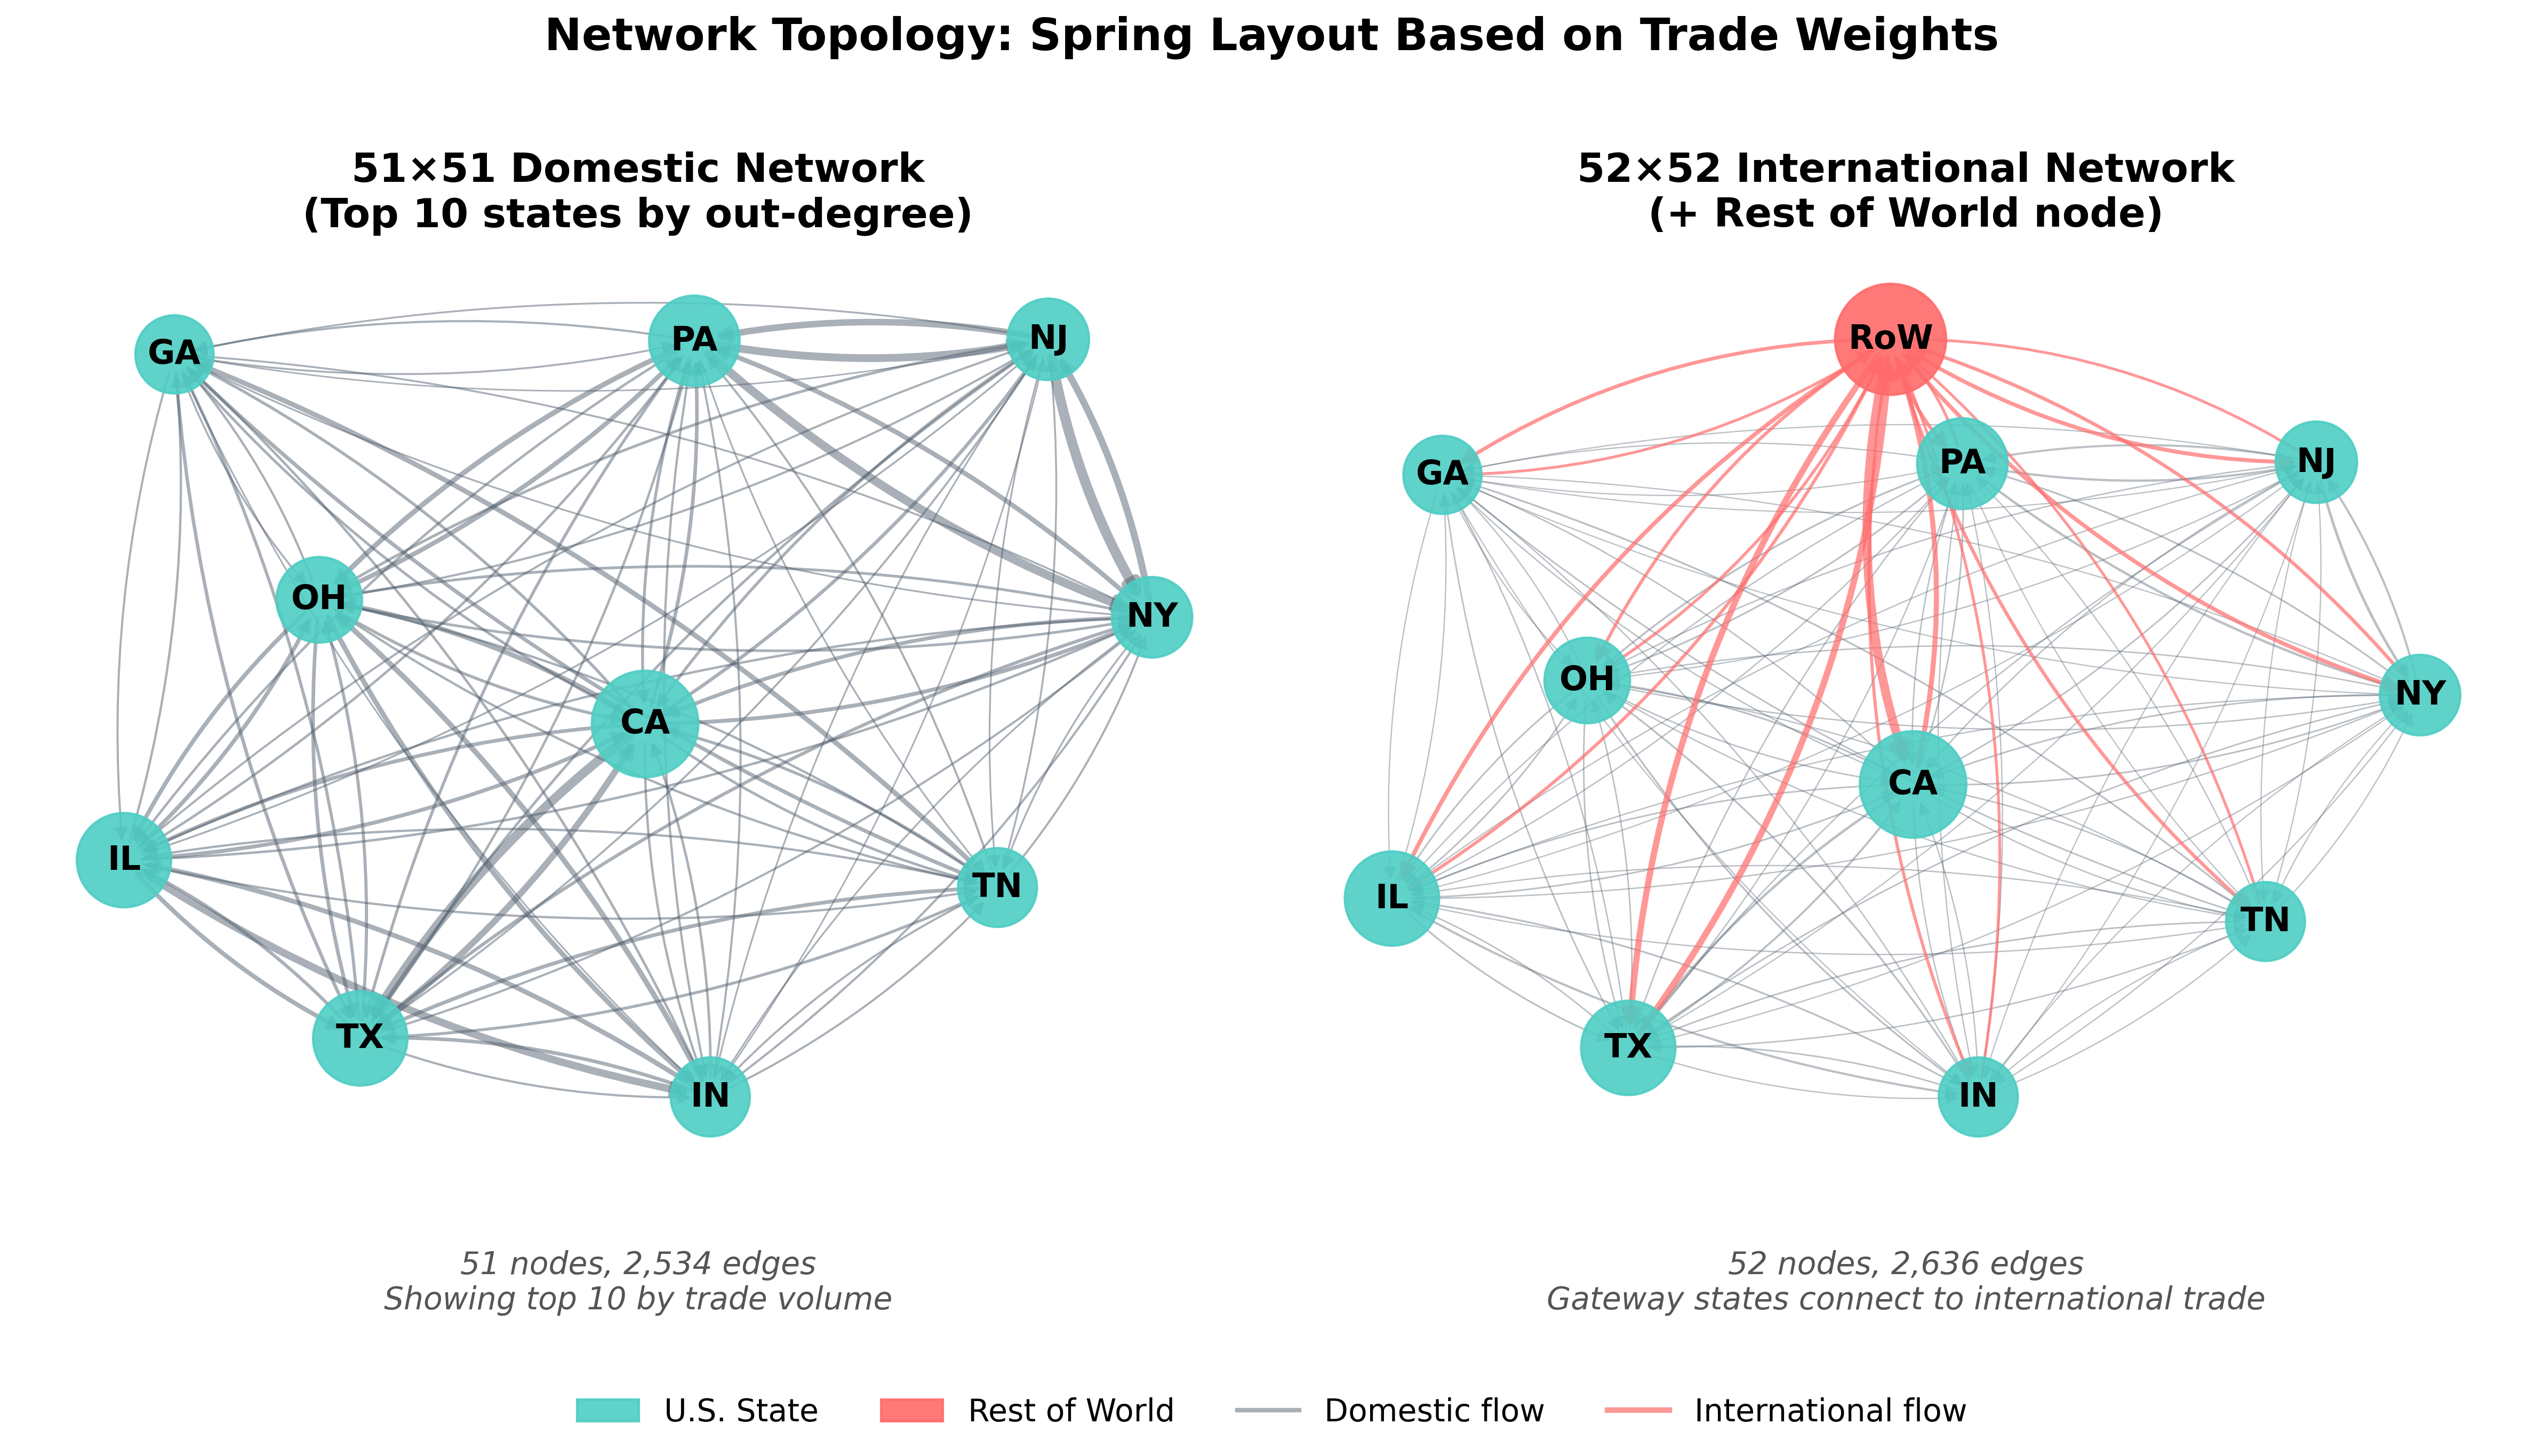
\includegraphics[width=\textwidth]{figures/network_construction_spring.png}
\caption[Network construction methodology showing actual network structure (top 10 states by out-degree centrality).]{Network construction methodology showing actual network structure (top 10 states by out-degree centrality). Left panel: 51×51 domestic baseline network with interstate flows only. Right panel: 52×52 internationally-integrated network with Rest of World (RoW) aggregate node added. Gateway states (CA, TX, NY, FL) shown with enhanced international connections when RoW is included.}
\label{fig:network_construction}
\end{figure}

We construct a weighted directed graph $G = (V, E, W)$ representing the U.S. system of interstate commodity trade flows, where:


\begin{itemize}
    \item $V$ is the set of 51 nodes (50 states + DC)
    \item $E \subseteq V \times V$ is the set of directed edges representing trade flows between states
    \item $W: E \to \mathbb{R}^{+}$ is a weight function that assigns each edge a positive value equal to the survey-adjusted trade flow between that state pair

  

\end{itemize}

Complete node distributions are provided in Appendix~\ref{appendix:node_distribution} and top bilateral flows in Appendix~\ref{appendix:edge_list}.

This graph is equivalently represented as a 51$\times$51 weighted adjacency matrix $\mathbf{A}$, which enables direct computation of eigenvector centrality and compact notation for all three centrality measures, where entry $A_{ij}$ represents the survey-weighted commodity flow value (in U.S. dollars) from state $i$ to state $j$. Unlike binary adjacency matrices that only record whether two states trade, this weighted representation preserves the economic magnitude of each relationship --- a \$50 billion flow carries more weight than a \$5 million flow.

To account for international trade flows, we construct a 52$\times$52 variant by adding a ``Rest of World'' (RoW) node representing the aggregate of each state's international exports and imports. This provides a means for boundary specification: comparing state rankings in the domestic only (51$\times$51) versus internationally integrated (52$\times$52) networks. Figure~\ref{fig:matrix_comparison} compares the adjacency matrix structure of both networks, revealing the additional row and column introduced by the RoW node and the concentration of international flows among a small number of gateway states.

\begin{figure}[ht]
\centering
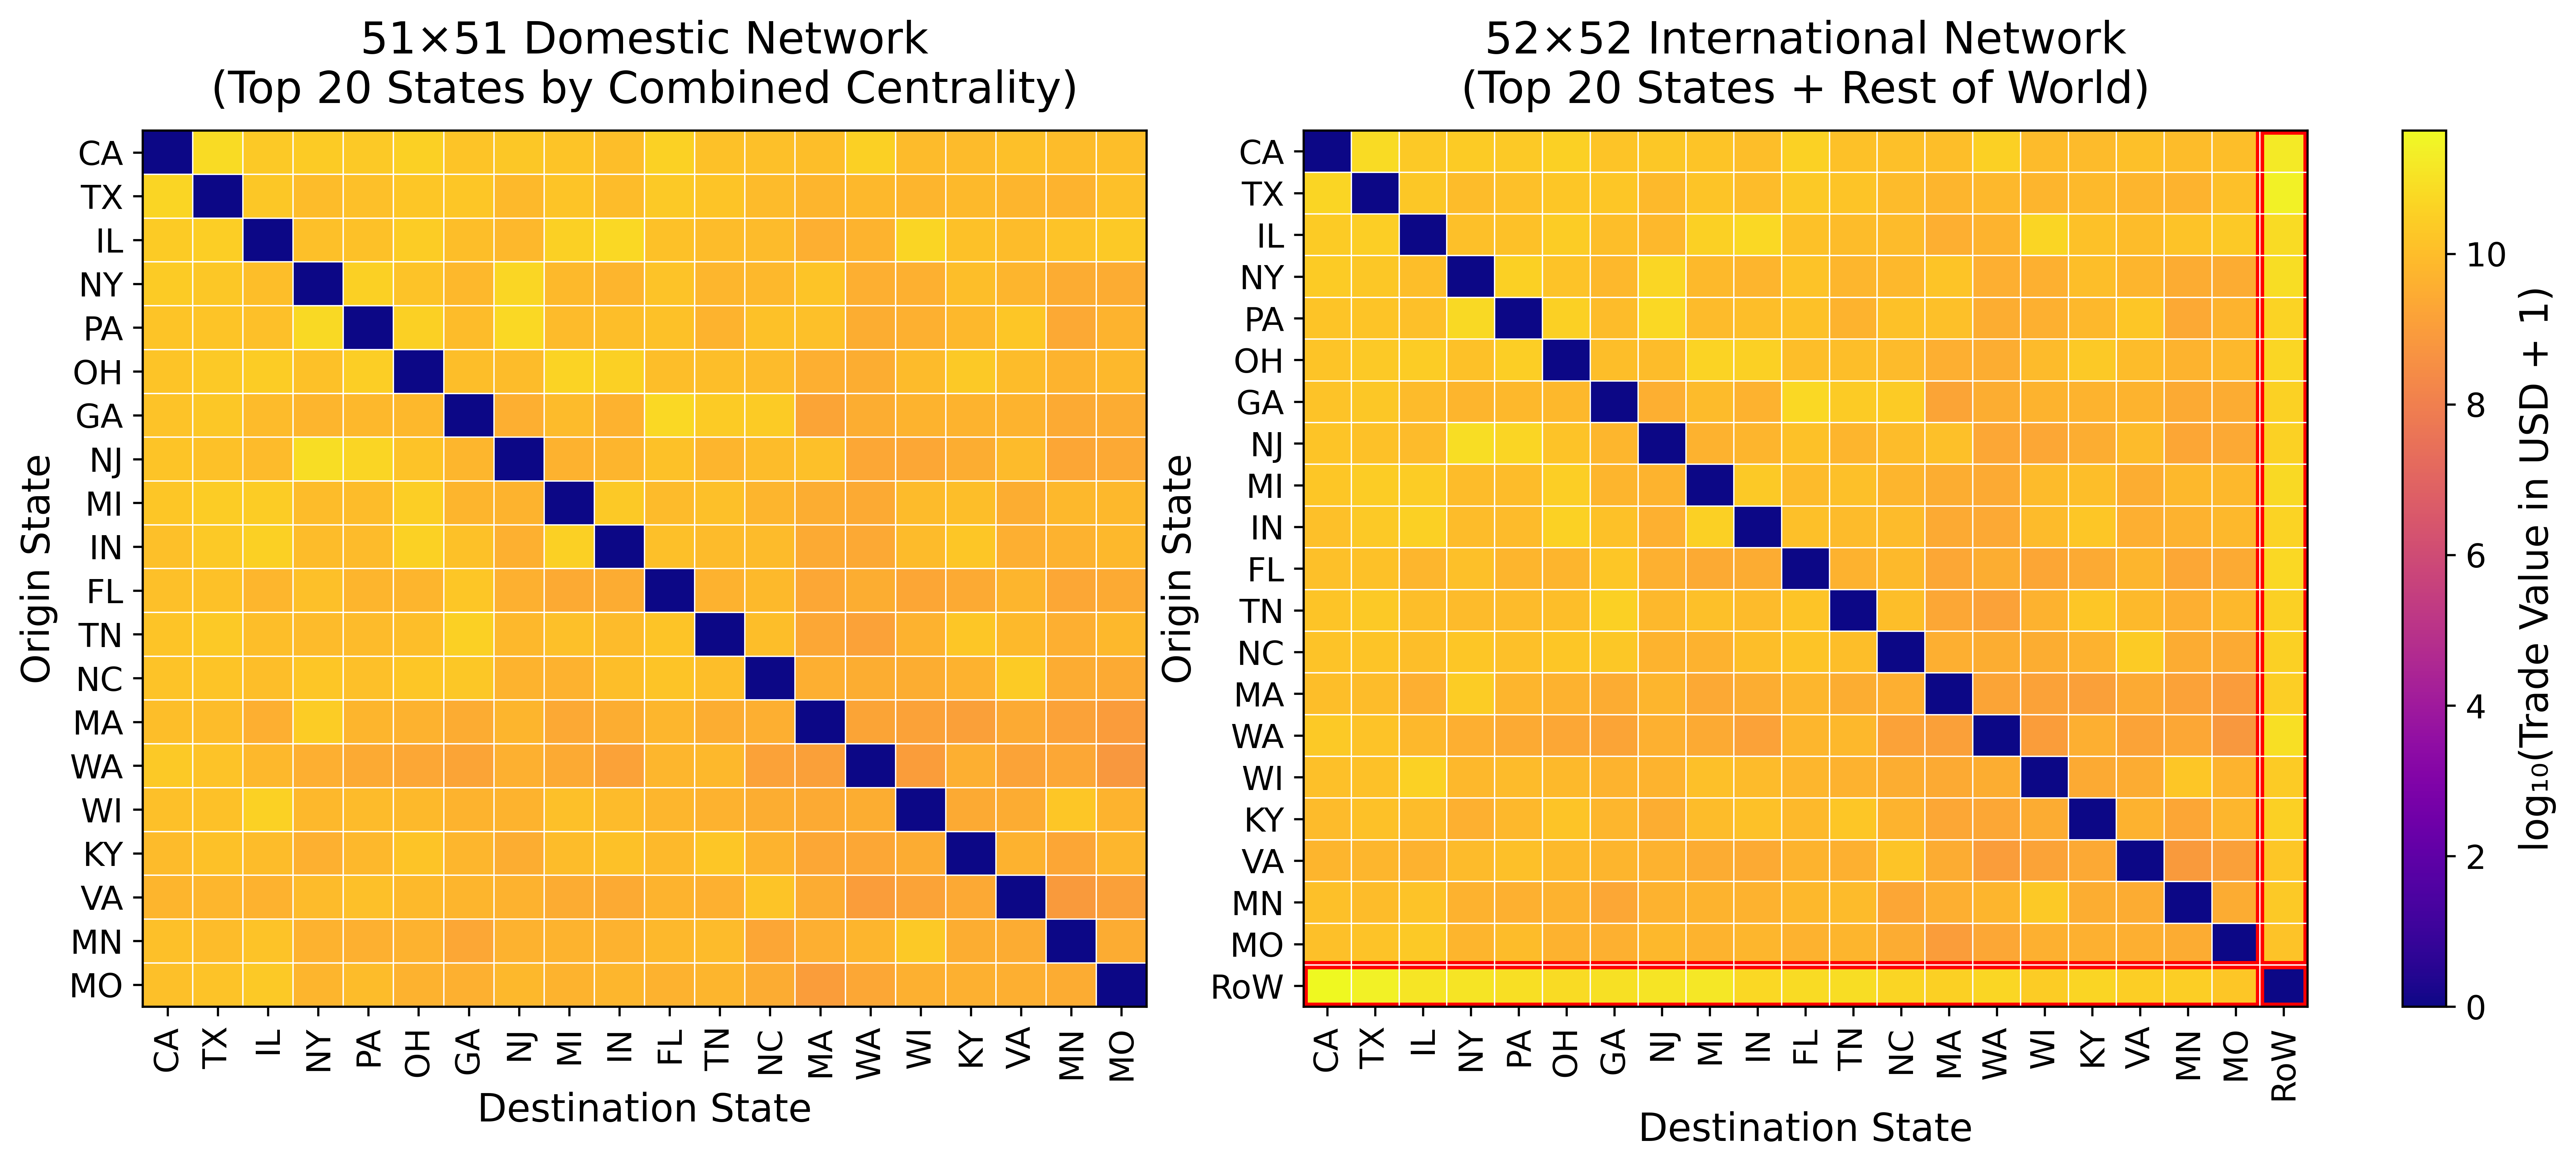
\includegraphics[width=\textwidth]{figures/matrix_comparison.png}
\caption[Matrix structure comparison showing top 20 states by aggregate centrality score.]{Matrix structure comparison showing top 20 states by aggregate centrality score (sum of min-max normalized betweenness, eigenvector, and out-degree). Left: 51×51 domestic network (interstate flows only). Right: 52×52 international-inclusive network with Rest of World (RoW) node. RoW highlighted with red border. Color scale (plasma) shows $\log_{10}$ of trade values in USD (e.g., 9 = \$1 billion, 10 = \$10 billion).}
\label{fig:matrix_comparison}
\end{figure}


The network construction preserves flow directionality and survey weighting while aggregating over commodity types, shipment-level detail, and temporal variation. Edge weights represent survey-adjusted trade values described in Section 3.1 and edge direction captures flow orientation (origin state $\to$ destination state). This lets us account for directional asymmetry (exports vs. imports) while ensuring economic magnitude informs centrality calculations.\footnote{A formal systems definition following Klir's framework \cite{klir_facets_2001} is provided in Appendix \ref{appendix:formal_system}.}

 

\section{Network Centrality Measures}

Three complementary centrality measures quantify structural power at macro, meso, and micro scales \cite{jang_measuring_2023} (Figure
\ref{fig:centrality_framework}). 

\begin{figure}[ht]
\centering
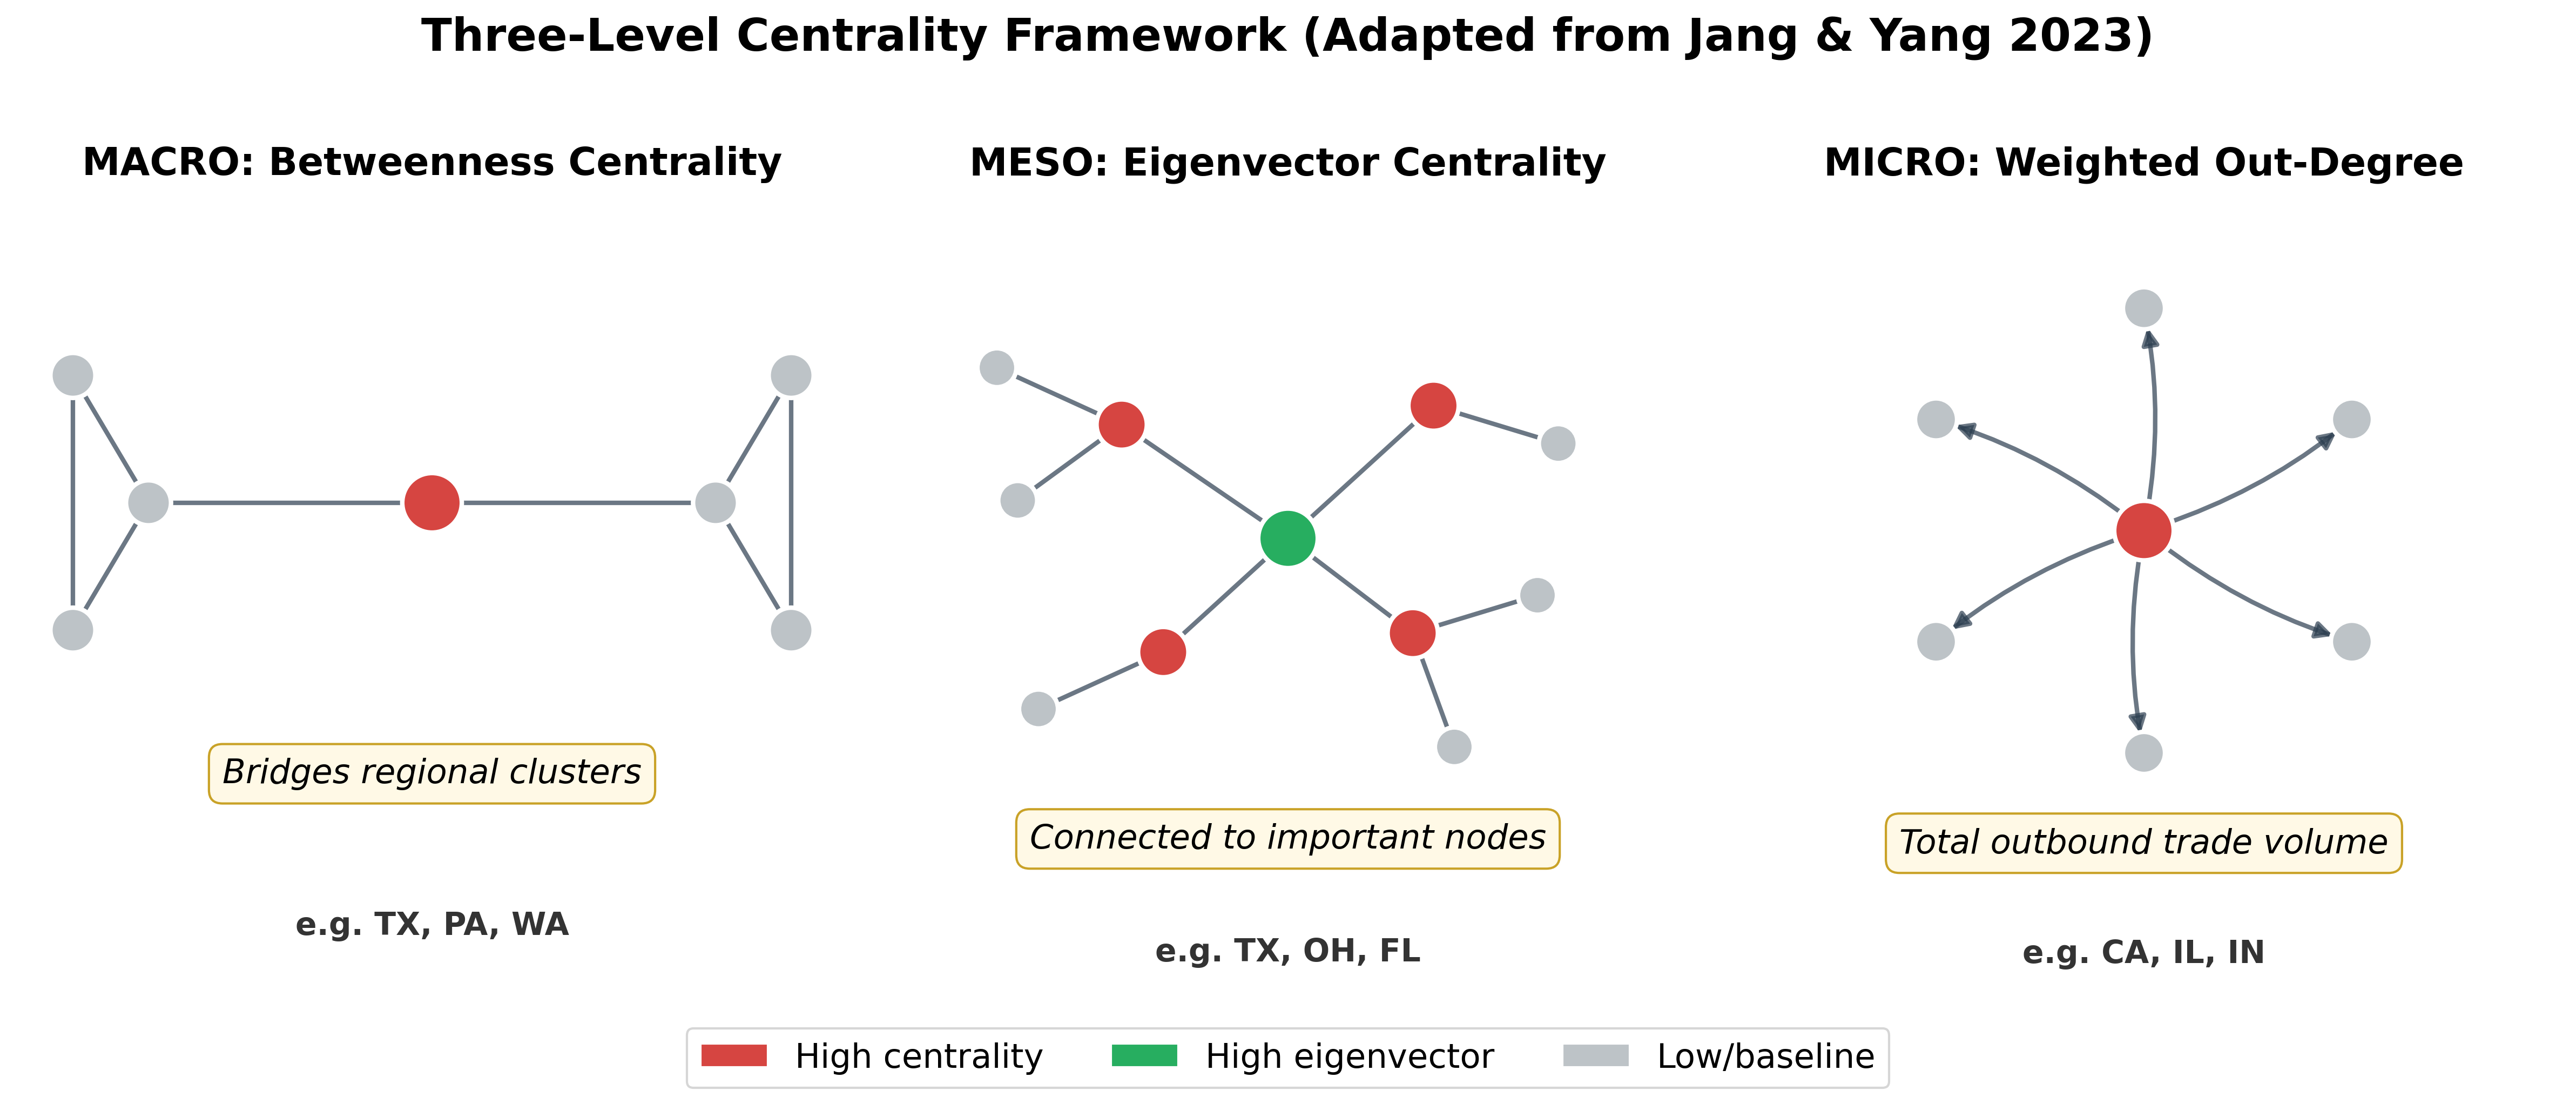
\includegraphics[width=\textwidth]{figures/centrality_framework_v2.png}
\caption[Three-level centrality framework adapted from Jang \& Yang (2023).]{Three-level centrality framework adapted from Jang \& Yang (2023). Highlighted nodes indicate centrality levels: red (high betweenness), green (high eigenvector), gray (low/baseline). Node size reflects relative centrality score.}
\label{fig:centrality_framework}
\end{figure}

\textbf{Betweenness Centrality} (macro-level bridging power) measures how often a state lies on shortest paths between other state pairs:

\begin{equation}
C_{B}(i)=\sum_{j \neq i \neq k} \frac{g_{jk(i)}}{g_{jk}}
\end{equation}

where $g_{jk}$ is the number of shortest paths between states $j$ and $k$, and $g_{jk(i)}$ is the number of those paths passing through state $i$ \cite{jang_measuring_2023}. For weighted shortest-path calculations, NetworkX treats edge weights as \textit{distances} rather than proximities. Since our adjacency matrix $\mathbf{A}$ encodes trade values where higher values indicate stronger connections, we invert weights before computing betweenness: $d_{ij} = w_{\max} / A_{ij}$. This transformation ensures shortest paths traverse high-volume trade corridors. Scores are normalized by dividing by the number of node pairs: $\frac{2}{(|V|-1)(|V|-2)}$ for directed graphs.


\textbf{Eigenvector Centrality} (meso-level influence) measures importance based on the strength of connections to other important states:

\begin{equation}
C_{E}(i)=\frac{1}{\lambda} \sum_{j=1}^{n} W_{i j} \cdot C_E(j)
\end{equation}

where $\lambda$ is the largest eigenvalue of the weighted adjacency matrix $\mathbf{A}$, $W_{ij}$ is the matrix element representing trade flow value from state $i$ to state $j$, and $C_E(j)$ is the eigenvector centrality of state $j$ \cite{jang_measuring_2023}. Intuitively, a state with high eigenvector centrality trades heavily with other economically important states, it is influential because its trading partners are influential. 

\textbf{Weighted Out-Degree} (micro-level distribution capacity) sums total outbound trade flows:

\begin{equation}
C_{D}(i)=\sum_{j=1}^{n} A_{ij}
\end{equation}

where $A_{ij}$ is the trade flow from state $i$ to state $j$. We focus on out-degree rather than in-degree because outbound flows capture a state's capacity to supply other states, a form of economic power through distribution. In-degree (imports) reflects dependency on other states rather than influence over them. This follows Jang \& Yang's emphasis on outward-directed measures of network power \cite{jang_measuring_2023}.

\section{Graph Filtration Analysis}

At 99.4\% density, the unfiltered 51$\times$51 network approaches a complete graph where nearly all state pairs trade directly --- it forms a single strongly connected component with no isolated nodes. In such near-clique structures, betweenness centrality in particular may reflect path optimization artifacts rather than genuine structural bridging. To validate centrality robustness in near-complete networks, we employ systematic edge removal (graph filtration). When every node connects to nearly every other node, shortest paths become trivially short and bridging roles are obscured. Filtration reveals which centrality patterns persist when weak edges are removed, distinguishing robust structural features from density artifacts.

Figure~\ref{fig:edge_weight_rank_distribution} ranks all 2,534 bilateral trade flows by descending value. The distribution exhibits a steep decline from the largest flow (\$78B, NJ$\to$NY) followed by a long tail of progressively smaller flows. This concentration is what motivates filtration: the long tail consists of edges that add connectivity without contributing meaningful structural information. The 33rd percentile threshold (\$298M) marks the maximum filtration level before network fragmentation. Filtering at this threshold removes 836 edges that collectively represent approximately 1\% of total trade value. The full 52$\times$52 weighted adjacency matrix is available in the supplemental data repository (see \url{https://github.com/rsthornton/us-trade-centrality/tree/main/data}). 

\begin{figure}[ht]
\centering
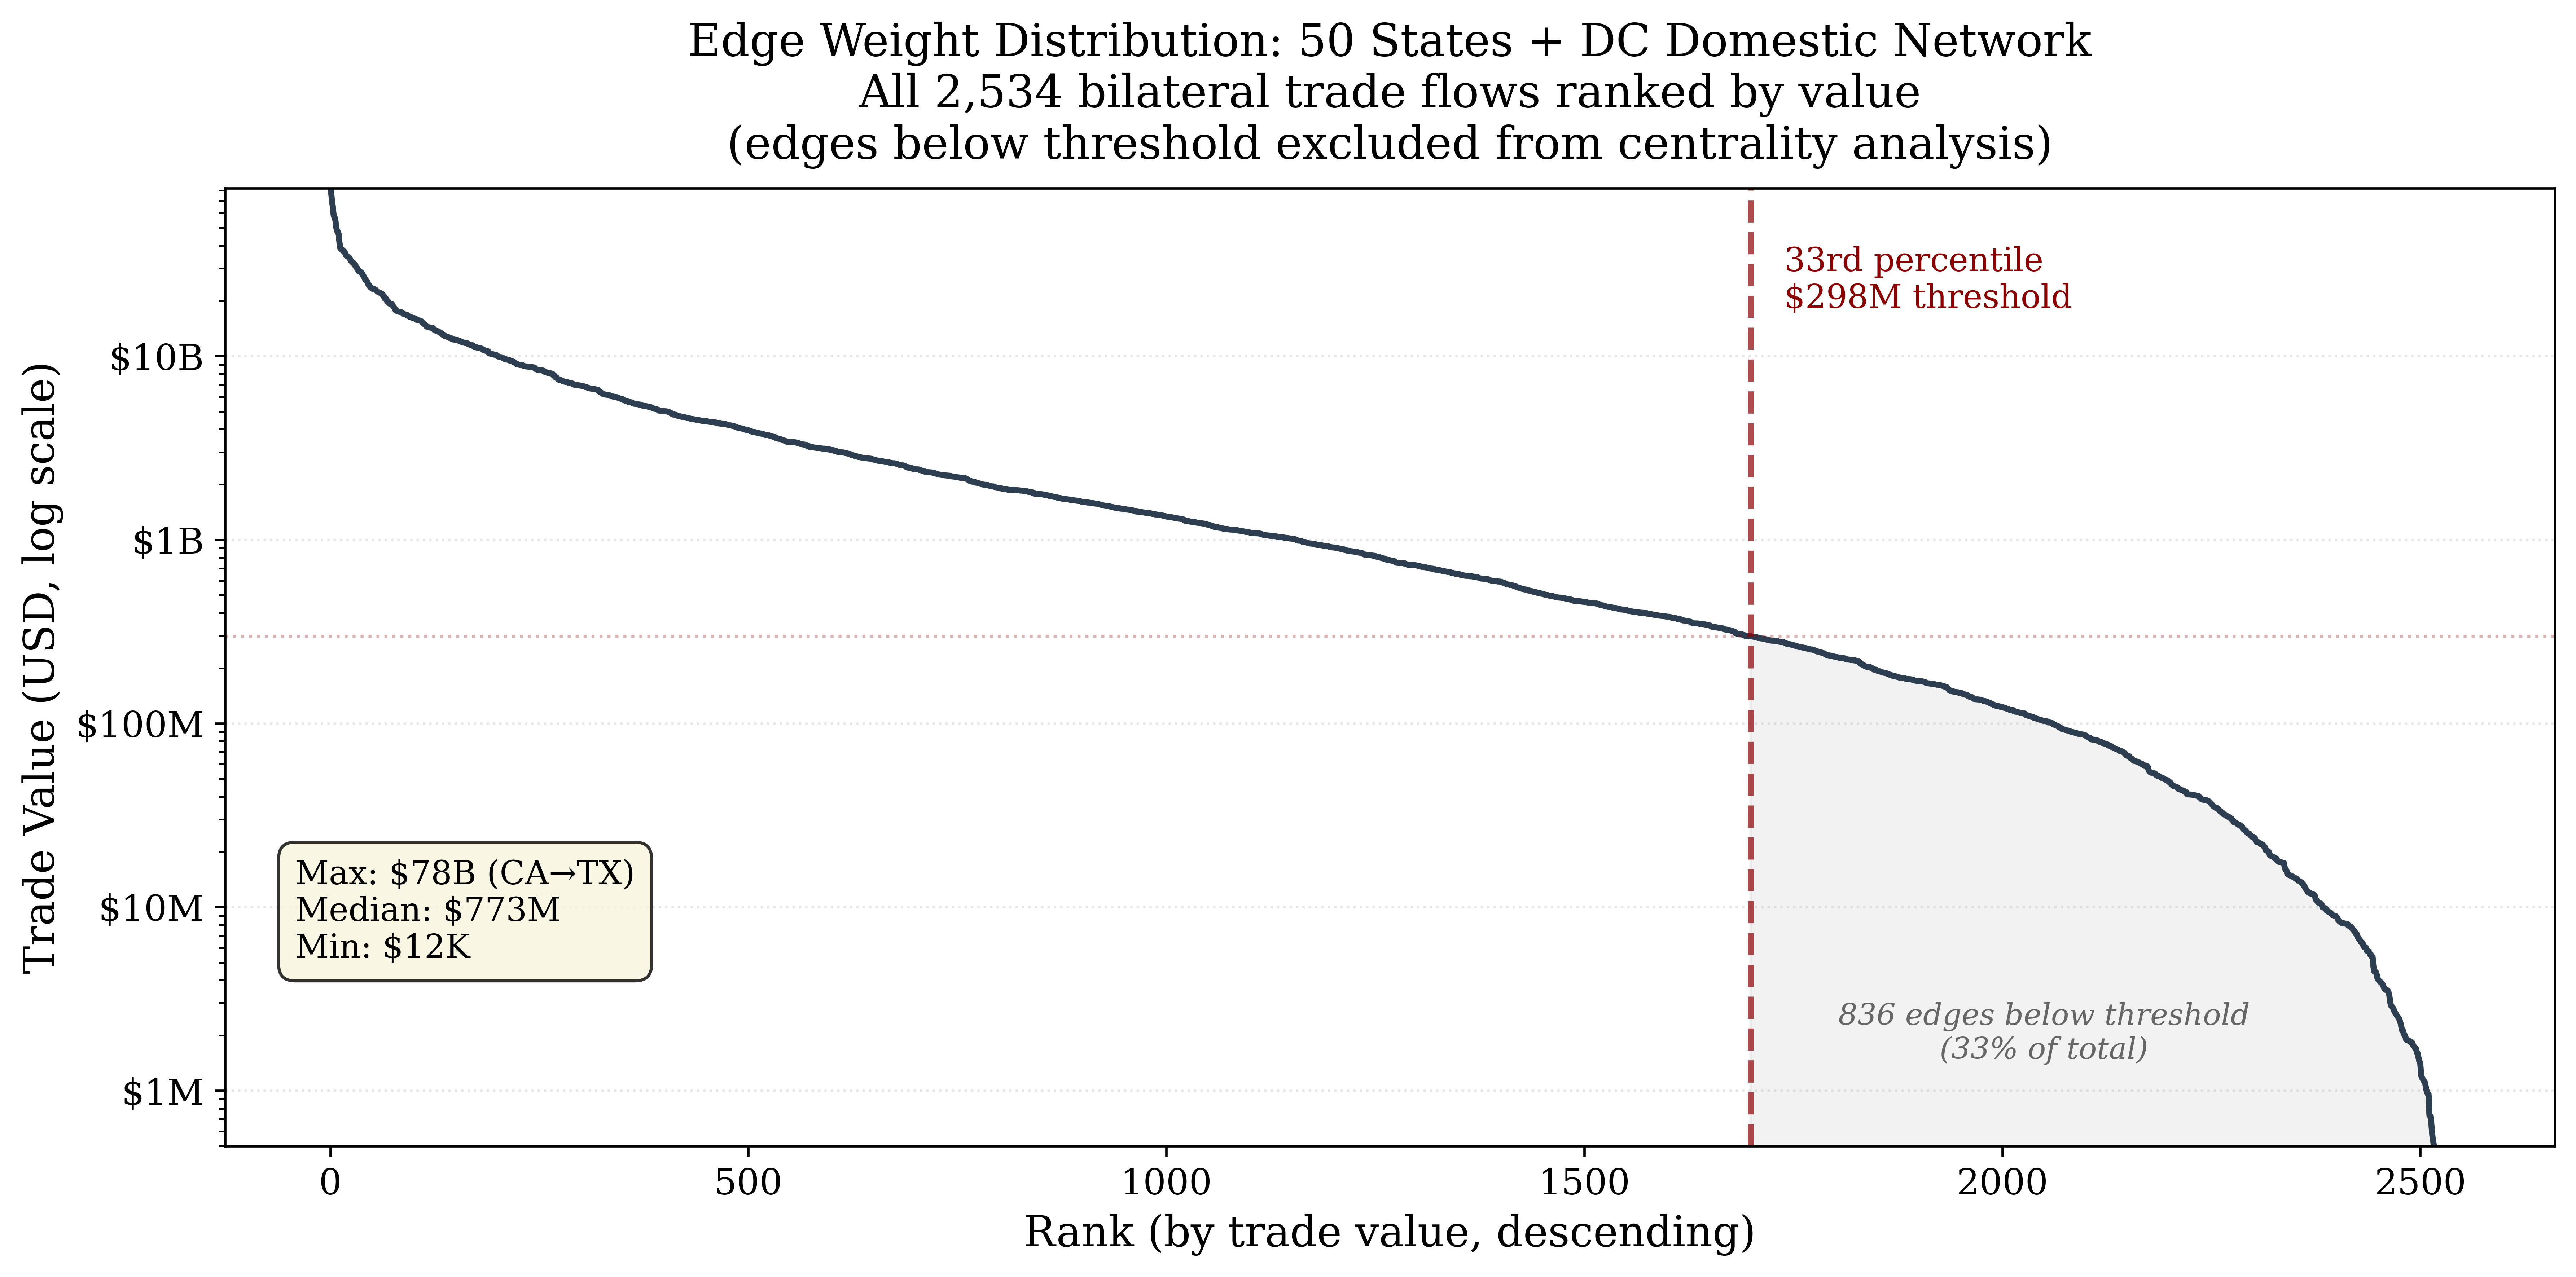
\includegraphics[width=\textwidth]{figures/edge_weight_rank_distribution.png}
\caption[Edge weight distribution for the 50 states + DC domestic network.]{Edge weight distribution for the 50 states + DC domestic network. All 2,534 bilateral trade flows ranked by descending value (log scale). Red dashed line marks the 33rd percentile cutoff (\$298M), the maximum filtration threshold before network fragmentation. Shaded region indicates edges removed during filtration.}
\label{fig:edge_weight_rank_distribution}
\end{figure}

Filtration proceeds by removing edges below a percentile threshold of edge weights and recomputing centrality on the resulting sparser graph. We use a systematic percentile sweep to identify the maximum filtration level that maintains a single strongly connected component, then analyze rank stability at that threshold. We track stability using Spearman correlation coefficients and measure how many states change positions. This analysis reveals whether high centrality derives from concentrated heavy flows (robust to filtration) or distributed weak connections (sensitive to filtration).

\section{Boundary Sensitivity Analysis}

To test whether state power rankings remain stable when international trade is included we systematically compare centrality measures between the 51$\times$51 and 52$\times$52 networks. We use four methods to quantify boundary effects. 

\begin{enumerate}
    \item \textbf{Network Validation.} Both networks are validated for structural integrity before comparison. Validation confirms each network forms a single strongly connected component (all states reachable from all others via directed paths), with no isolated nodes and density exceeding 0.99 (meaning over 99\% of all possible directed edges exist).

    \item \textbf{Rank Correlation.} Spearman rank correlation coefficients ($\rho$) quantify the relationship between state rankings in the two networks for each centrality measure. Values above 0.95 indicate high ranking stability; values below 0.90 suggest meaningful boundary effects.

    \item \textbf{Rank Change Analysis.} For each state and measure, rank changes are computed as the difference between 51×51 and 52×52 positions. Summary statistics include mean absolute rank change, maximum rank change, and percentage of states that changed rank. Changes exceeding 2 positions are considered meaningful given the 51-state ranking scale.

    \item \textbf{Top-K Overlap.} Top-$k$ overlap measures whether the same states occupy leadership positions in both networks. For each threshold $k$ (top-5, top-10, top-20), $O_k = |S_{51} \cap S_{52}| / k$, where $S_{51}$ and $S_{52}$ are the top-$k$ states in each network. Values below 0.6 indicate substantial leadership turnover due to boundary specification.
    

\end{enumerate}

\section{Limitations and Scope}

This analysis only examines state economic centrality through commodity trade flows.

First, the scope of power measurement. The analysis measures economic centrality in commodity trade networks, not comprehensive state power. It excludes various other economic, fiscal, political, social, and cultural dimensions that would be needed for a more comprehensive evaluation of power.

Second, geographic and temporal boundaries introduce further constraints. State-level aggregation masks within-state variation, for example California's ports versus the Central Valley which have different roles that this analysis cannot distinguish. The Rest of World node aggregates all international partners into a single entity which obscures the complex heterogeneity in international relationships. Additionally, this analysis focuses on a single year, 2017. The temporal dynamics highlighted by Jang \& Yang, who examined global trade network data from 1996 to 2020, are not examined here. 

Third, there are data constraints. The analysis focuses solely on commodity flows, excluding services trade, financial flows, and information exchange. Survey-based data may be subject to sampling error and reporting biases even though census validation procedures mitigate these concerns. All 43 SCTG commodity categories are aggregated into total trade flows between state pairs. The SCTG system classifies physical goods broadly, encompassing both raw materials (e.g., agricultural products, minerals) and manufactured items (e.g., machinery, electronics), but excludes services.

Finally, the methodological choices introduce constraints. Betweenness centrality uses weighted edges where high trade value corresponds to short distances. Alternative edge weighting schemes (e.g., tonnage or shipment count) might reveal different bridging patterns and merit future investigation. The 52$\times$52 specification provides just one of many potential boundary extensions; others (regional, modal, sectoral) were not explored.

\chapter{Results}

\section{Network Properties}

The 51×51 domestic network contains 51 nodes (50 states plus DC) with 2,534 directed edges representing \$7.6 trillion in interstate commodity flows. The network is strongly connected with density 0.994 (2,534 of 2,550 possible edges) and diameter 2 (any state can reach any other in at most two steps). Nearly all trade relationships are bidirectional: 99.4\% of edges are reciprocal, meaning states that export to a partner almost always import from that partner. The 16 missing edges (0.6\% of possible connections) follow a clear pattern: 15 are DC outflows to smaller states. WY-DC is the only state pair with no trade in either direction. The top bilateral trade flows are listed in Appendix~\ref{appendix:edge_list}. The complete set of all 2,534 bilateral flows is available in the supplemental data repository (see \url{https://github.com/rsthornton/us-trade-centrality/tree/main/data}).

The 52$\times$52 international inclusive network contains 52 nodes (adding Rest of World) with 2,636 edges representing \$11.4 trillion in total flows. This network maintains similar structural properties: density 0.994, diameter 2, and reciprocity 99.4\%. RoW exhibits high centrality, ranking first for both eigenvector and out-degree centrality in the international network. This matters for boundary sensitivity (Section~\ref{sec:international}): when RoW dominates eigenvector and out-degree rankings, it also reshapes the shortest paths that determine betweenness. 

Both networks exhibit near-complete connectivity (99.4\% density) with minimal path lengths, indicating highly integrated commerce systems. Table~\ref{tab:network_properties} summarizes the structural properties of both networks. Despite the addition of international flows---which increase total trade value from \$7.6T to \$11.4T---density, diameter, and reciprocity remain essentially unchanged. This confirms that the RoW node integrates into an already highly connected system rather than altering its network structure. 

\begin{table}[ht]
  \centering
  \caption[Network Properties Comparison (51 $\times$ 51 Domestic vs.\ 52 $\times$ 52 International).]{Network Properties Comparison (51 $\times$ 51 Domestic vs. 52 $\times$ 52 International). The 52 $\times$ 52 network includes
  international flows, adding \$3.8T in trade value while preserving structural properties.}
  \label{tab:network_properties}
  \begin{tabular}{lcc}
  \hline
  \textbf{Property} & \textbf{51×51 Domestic} & \textbf{52×52 International} \\
  \hline
  Nodes & 51 & 52 \\
  Edges & 2,534 & 2,636 \\
  Total Value & \$7.6T & \$11.4T \\
  Density & 0.994 & 0.994 \\
  Diameter & 2 & 2 \\
  Reciprocity & 99.4\% & 99.4\% \\
  Avg. Path Length & 1.01 & 1.01 \\
  \hline
  \end{tabular}
\end{table}


\section{Filtration Analysis: Validating Centrality Robustness}
\label{sec:filtration}

At 99.4\% density, the domestic network is nearly complete. Do these rankings reflect genuine structural patterns or artifacts of weak connections?
This question is especially important for betweenness centrality, which Segarra \& Ribeiro \cite{segarra_stability_2015} proved mathematically discontinuous in dense networks under standard distance-based computation. Before interpreting centrality rankings, we test their robustness through systematic edge removal (graph filtration). 

As the edge weight distribution shows (Figure~\ref{fig:edge_weight_rank_distribution}), the network exhibits extreme flow concentration: a few edges carry most of the trade value. Median bilateral flow is \$773M, mean is \$3.0B, maximum exceeds \$78B. We apply 33\% filtration, removing edges below the 33rd percentile (\$298M threshold). This is the maximum threshold before fragmentation---the network breaks into multiple components at 34\% (\$323M). Table~\ref{tab:filtration_sensitivity} presents the results: all three centrality measures maintain $\rho = 1.000$ with zero rank changes. Rankings are driven entirely by edges above the 33rd percentile, confirming that the observed centrality rankings reflect the network's high-value backbone rather than low-weight edge noise. 

\begin{table}[ht]
\centering
\caption[Centrality Rank Stability Under Graph Filtration (51 $\times$ 51 Domestic Network).]{Centrality Rank Stability Under Graph Filtration (51 $\times$ 51 Domestic Network). With weight inversion applied, all centrality measures remain perfectly stable under 33\% filtration. This demonstrates that the three-level centrality framework captures genuine structural patterns robust to methodological choices about weak-edge treatment.}
\label{tab:filtration_sensitivity}
\begin{tabular}{lccc}
\hline
\textbf{Centrality} & \textbf{Spearman $\rho$} & \textbf{Top-5 Stability} & \textbf{States Changed} \\
\textbf{Measure} & \textbf{(Full vs. 33rd \%ile)} & & \\
\hline
Betweenness   &  1.000  & 100\% &  0/51 (0\%) \\
Eigenvector   &  1.000  & 100\% &  0/51 (0\%) \\
Out-Degree    &  1.000  & 100\% &  0/51 (0\%) \\
\hline
\end{tabular}
\end{table}

All three centrality measures demonstrate perfect stability under filtration (Table~\ref{tab:filtration_sensitivity}): betweenness, eigenvector, and out-degree maintain $\rho = 1.000$ with no rank changes. This stability depends on how edge weights are treated. 
NetworkX treats edge weights as distances by default, so high trade values must be inverted to short distances before computing betweenness (see Section~\ref{sec:methods} for implementation details).

Table~\ref{tab:filtration_properties} shows how filtration changes the network's structural properties. While node count remains constant (all 51 states remain in the network), removing the weakest third of edges reduces density from 0.994 to 0.666 and increases diameter from 2 to 3. The increase in average path length from 1.006 to 1.338 confirms that filtration reveals the backbone structure: states that were trivially reachable through weak connections now require routing through major trade hubs, making betweenness centrality a meaningful measure of intermediary importance.  

\begin{table}[ht]
  \centering
  \caption[Network Properties Before and After 33\% Graph Filtration (51$\times$51 Domestic Network).]{Network Properties Before and After 33\% Graph Filtration (51$\times$51 Domestic Network). Filtration removes edges below the 33rd percentile (\$298M threshold), the maximum level before network fragmentation.}
  \label{tab:filtration_properties}
  \begin{tabular}{lcc}
  \hline
  \textbf{Property} & \textbf{Full Network} & \textbf{Filtered (33\%)} \\
  \hline
  Nodes & 51 & 51 \\
  Edges & 2,534 & 1,698 \\
  Density & 0.994 & 0.666 \\
  Diameter & 2 & 3 \\
  Avg.\ Path Length & 1.006 & 1.338 \\
  Reciprocity & 0.994 & 0.898 \\
  \hline
  \end{tabular}
\end{table}


\section{Domestic Network: Structural Position vs. Economic Size}
\label{sec:domestic}

Does network centrality reveal structural patterns that GDP alone cannot? This question (RQ1) is central to justifying network analysis of trade systems. If centrality merely reflects economic size, standard GDP metrics would suffice. To test this, we compare centrality rankings to GDP rankings using rank divergence analysis. We first verify that GDP serves as an appropriate baseline for economic size: GDP and population correlate at $r = 0.98$ (Pearson), indicating that normalizing by GDP effectively controls for both economic output and population. Because this analysis compares \textit{rankings} rather than raw scores, normalization method does not affect results. Dividing all scores by the same constant preserves ordering. 

We then define \textit{rank divergence} as:
\[
\Delta_i = \text{rank}_{\text{GDP}}(i) - \text{rank}_{\text{centrality}}(i)
\]
Positive divergence indicates a state is more central than its GDP predicts (``punches above its weight''); negative divergence indicates structural underperformance relative to economic size.

\subsection{How Much Does Centrality Mirror GDP?}

Eigenvector centrality correlates strongly with GDP ($\rho = 0.934$), as does out-degree ($\rho = 0.904$). Betweenness diverges: at $\rho = 0.763$, it captures something GDP does not. Population produces nearly identical rankings (GDP--population $r = 0.98$), so we use GDP as our baseline throughout. All seven centrality--control scatter plots are in Appendix~\ref{appendix:scatters}.

Table~\ref{tab:top10} presents raw centrality rankings for reference.

\begin{table}[ht]
    \centering
    \caption[Top 10 States by Centrality Measure (51 $\times$ 51 Domestic Network).]{Top 10 States by Centrality Measure (51 $\times$ 51 Domestic Network).
    Shaded cells indicate states appearing in all three top-10 lists.}
    \label{tab:top10}
    \begin{tabular}{clll}
    \hline
    \textbf{Rank} & \textbf{Betweenness} & \textbf{Eigenvector} & \textbf{Out-Degree} \\
    \hline
    1 & \textbf{\cellcolor{gray!15}CA} & \textbf{\cellcolor{gray!15}TX} & \textbf{\cellcolor{gray!15}CA} \\
    2 & \cellcolor{gray!15}TX & \cellcolor{gray!15}CA & \cellcolor{gray!15}TX \\
    3 & NY & NY & \cellcolor{gray!15}IL \\
    4 & \cellcolor{gray!15}PA & \cellcolor{gray!15}OH & \cellcolor{gray!15}PA \\
    5 & \cellcolor{gray!15}IL & FL & \cellcolor{gray!15}OH \\
    6 & MA & \cellcolor{gray!15}IL & NJ \\
    7 & \cellcolor{gray!15}OH & \cellcolor{gray!15}PA & NY \\
    8 & WA & MI & IN \\
    9 & MN & NJ & TN \\
    10 & \cellcolor{gray!15}GA & IN & \cellcolor{gray!15}GA \\
    \hline
    \end{tabular}
\end{table}

\clearpage
\subsection{Structural Divergence}

Florida ranks 4th in GDP (\$984B) but lies on no shortest paths in the trade network. It has zero betweenness centrality. More broadly, 39\% of states diverge by five or more rank positions between GDP and eigenvector centrality. Figure~\ref{fig:gdp_scatter} visualizes rank divergence for all 51 states. States above the diagonal achieve higher centrality than their GDP predicts; states below underperform structurally relative to economic size. By eigenvector divergence, the top overperformers are KY (+14), MS (+10), MT (+8), LA (+7), SC (+7), TN (+6), MI (+6), and IN (+6). These states share a common profile: manufacturing, energy, and agriculture. Their network importance exceeds what GDP alone predicts. 

\begin{figure}[H]
\centering
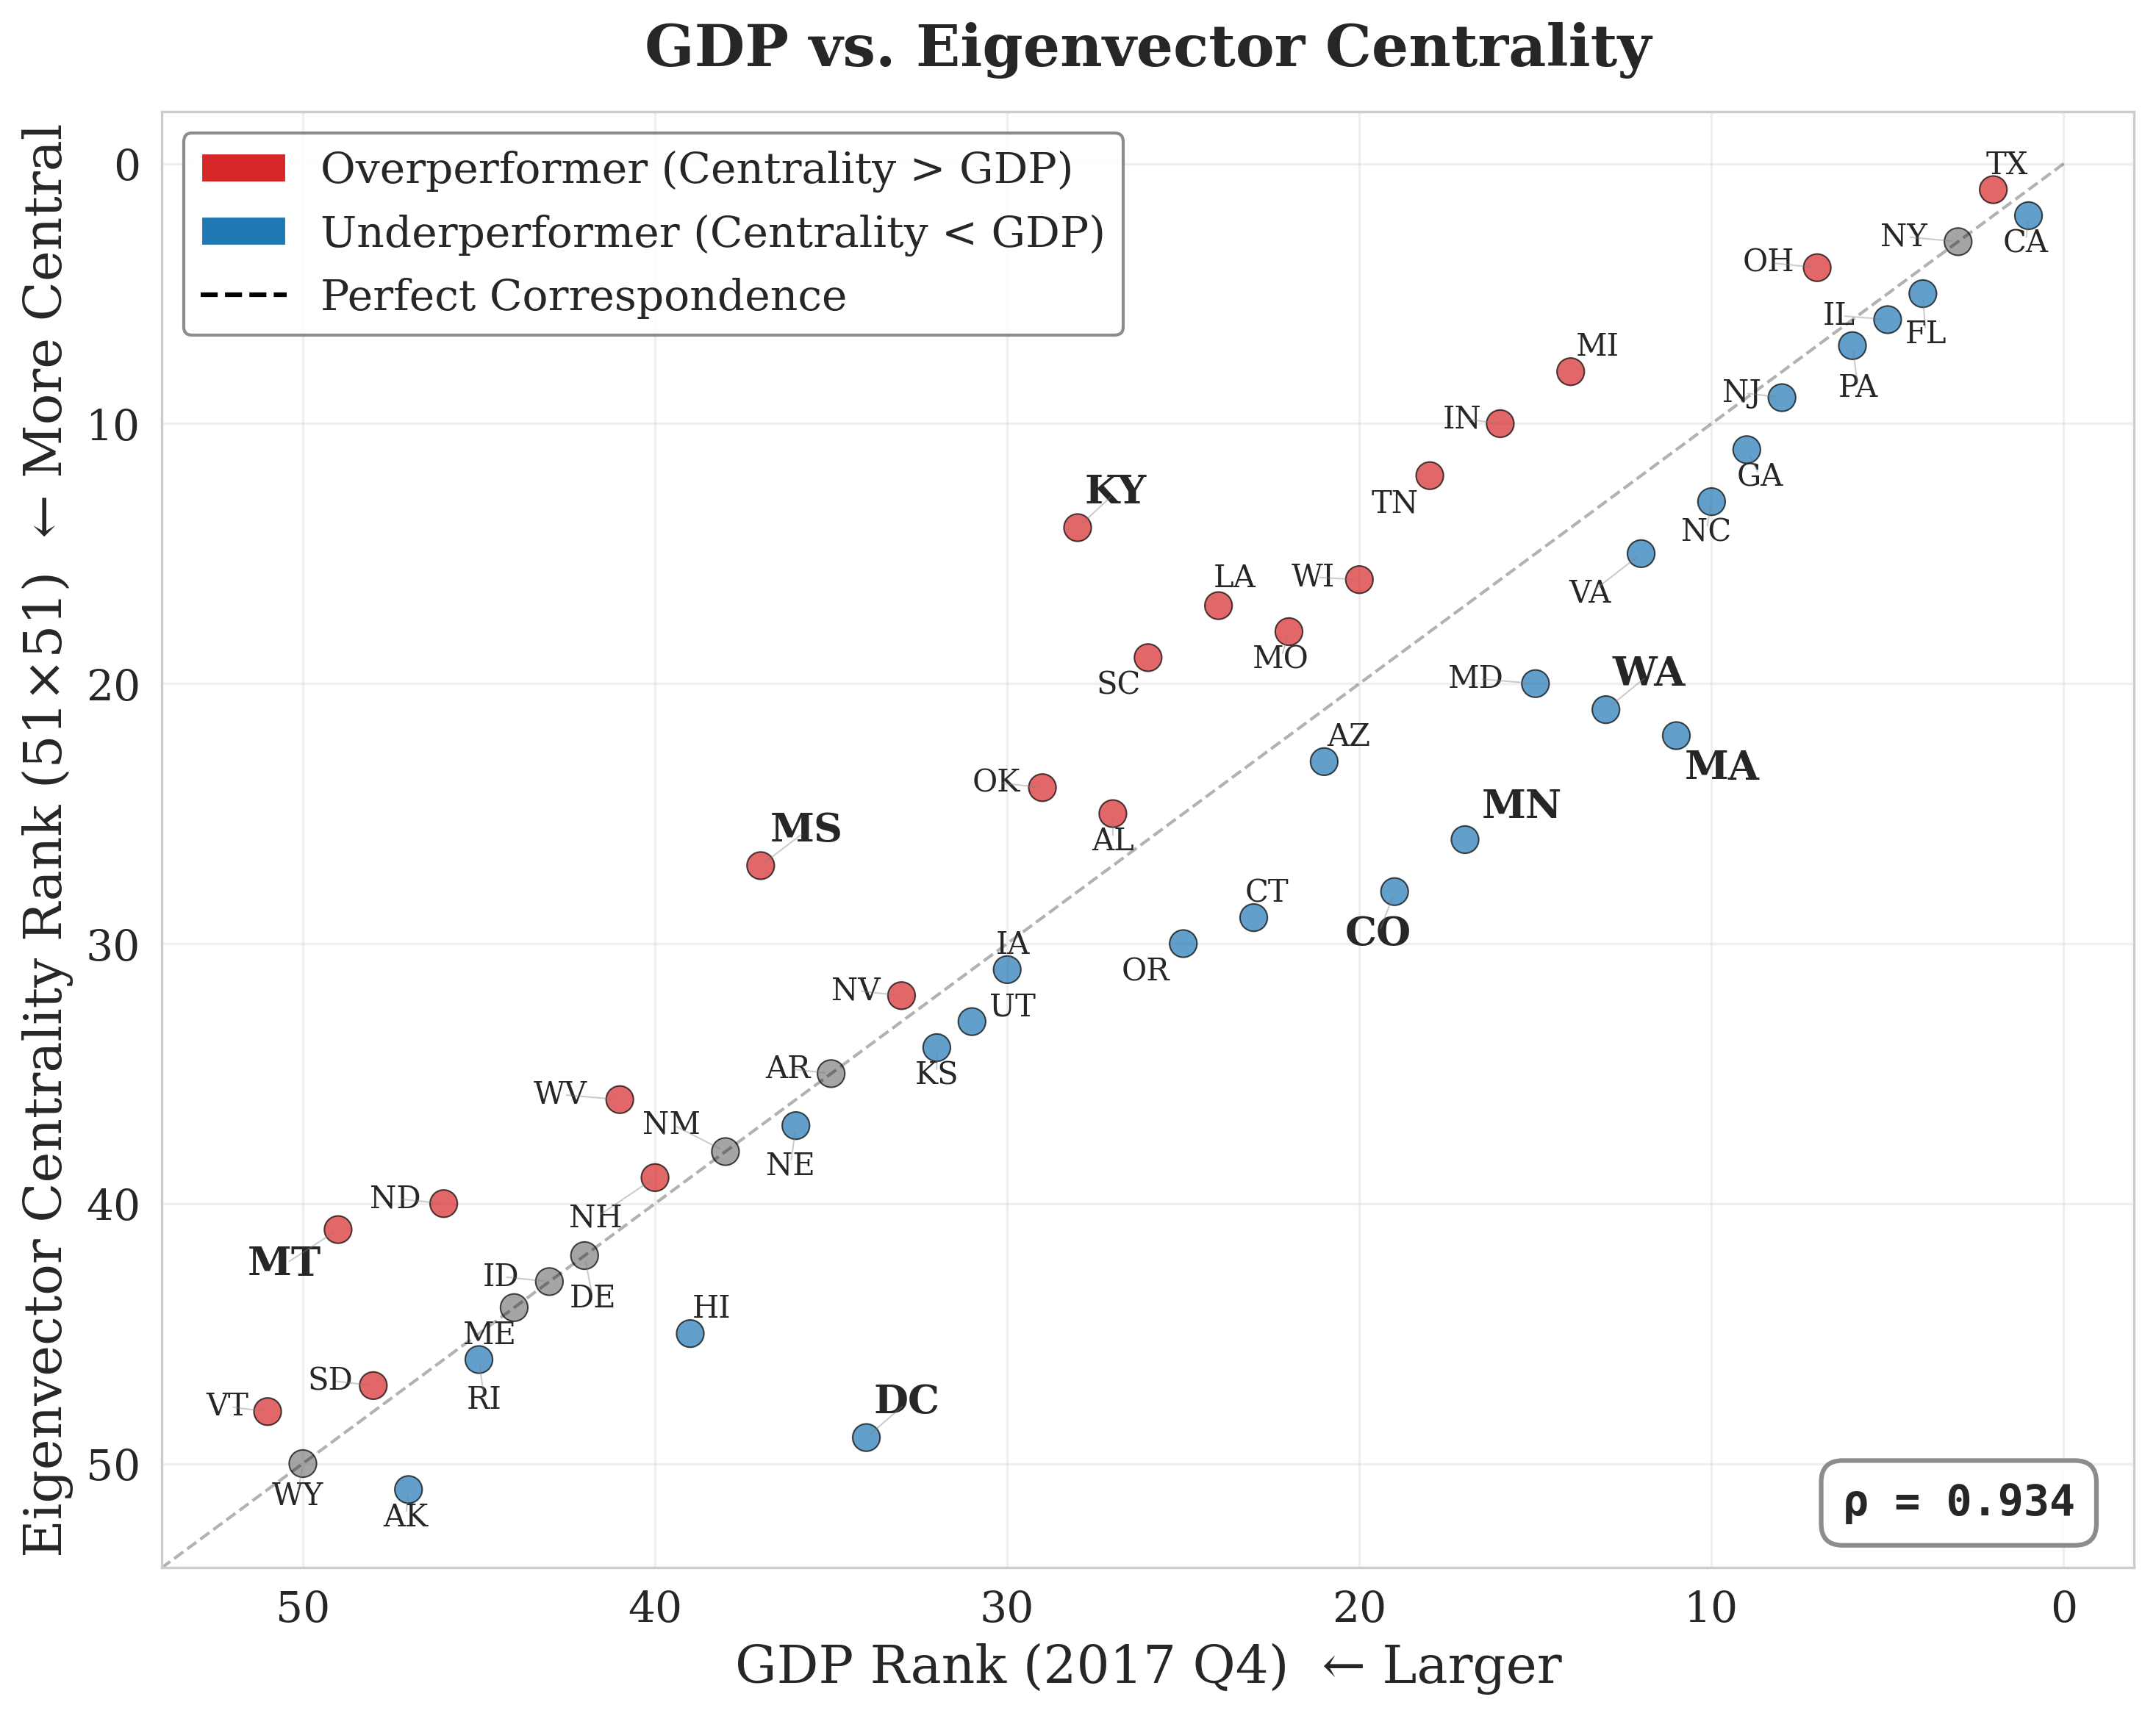
\includegraphics[width=\textwidth]{figures/gdp_vs_eigenvector_scatter.png}
\caption[GDP rank versus eigenvector centrality rank (Spearman $\rho = 0.934$).]{GDP rank versus eigenvector centrality rank (Spearman $\rho = 0.934$). States above diagonal rank higher in centrality than GDP predicts (structural overperformers). States below diagonal rank lower (structural underperformers). Labels show states with rank difference $\geq$ 8 positions. Additional scatter plots for all centrality--control combinations are in Appendix~\ref{appendix:scatters}.}
\label{fig:gdp_scatter}
\end{figure}


The most divergent underperformers are DC (-15), MA (-11), MN (-9), CO (-9), and WA (-8). These states have service-oriented or technology-focused economies; the CFS measures physical commodity shipments, not the services and software that drive these economies. When centrality is normalized by GDP, the pattern sharpens. Mississippi achieves the highest centrality per billion dollars GDP (0.000672), followed by Kentucky (0.000658) and Indiana (0.000551). Figure~\ref{fig:gdp_normalized} shows GDP-normalized eigenvector centrality for the top 15 states. 



\begin{figure}[H]
\centering
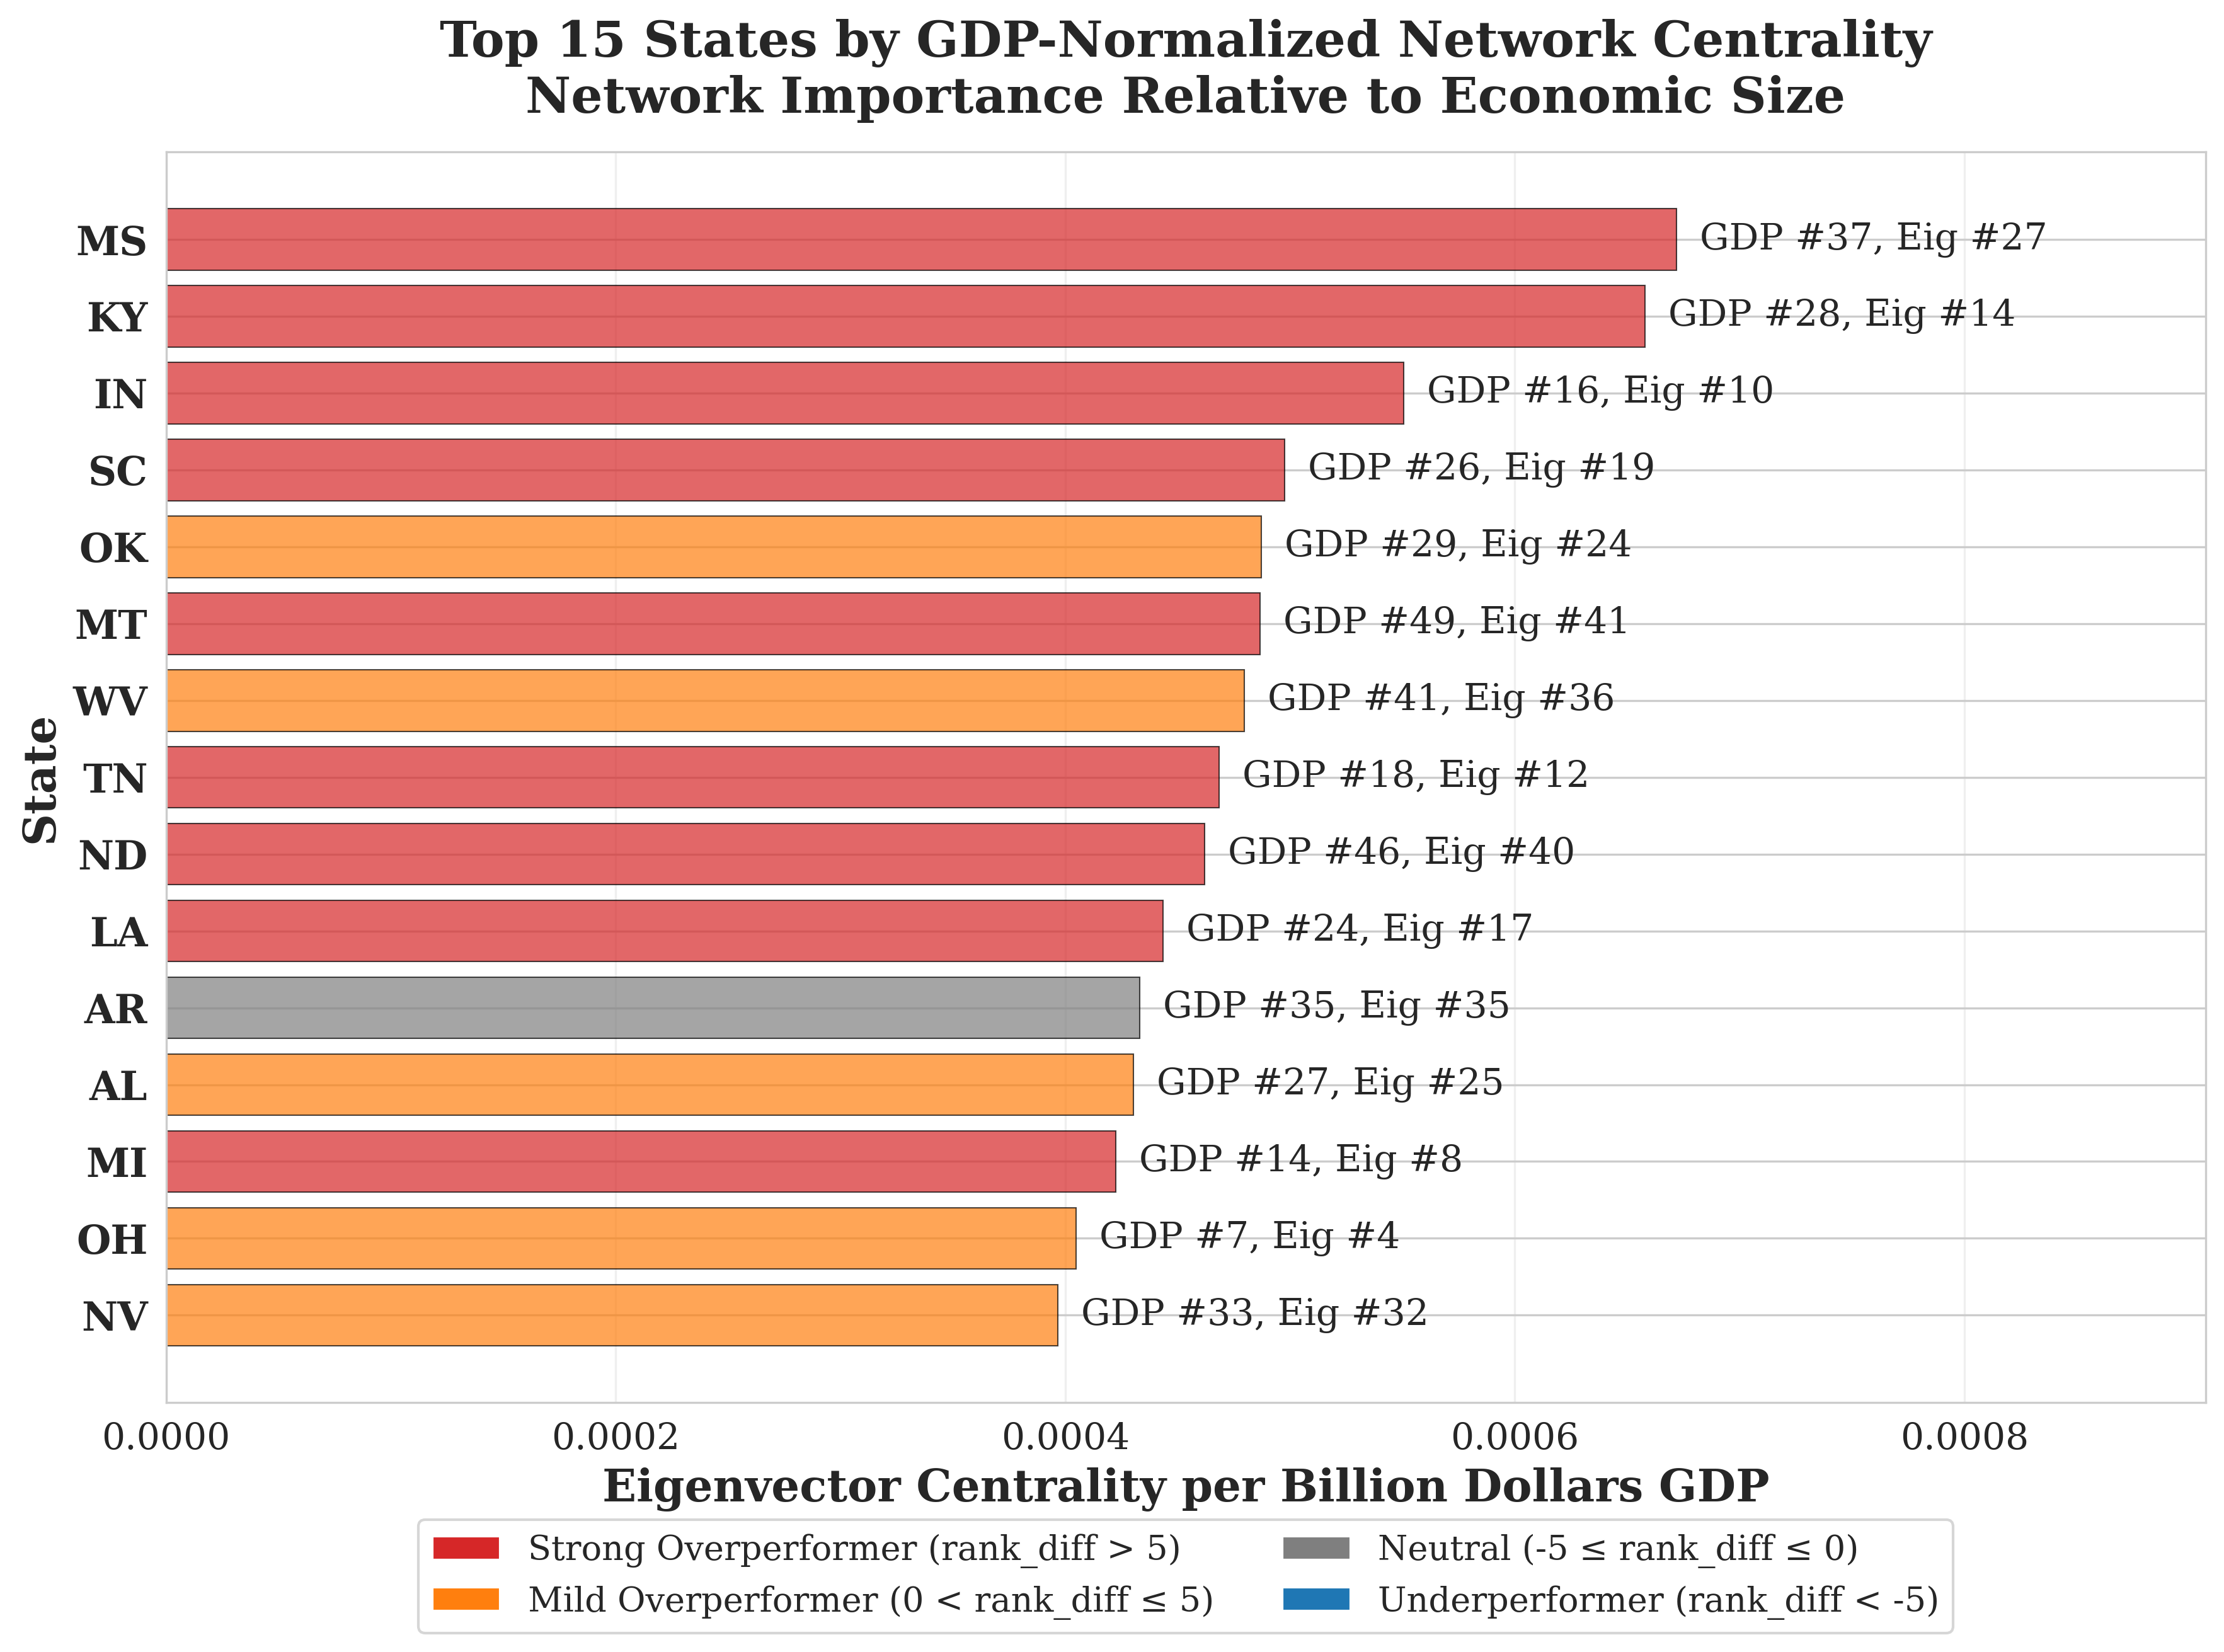
\includegraphics[width=\textwidth]{figures/gdp_normalized_centrality_bar.png}
\caption[Top 15 states by GDP-normalized eigenvector centrality.]{Top 15 states by GDP-normalized eigenvector centrality. Bars show centrality per billion 2017 GDP. Colors indicate rank divergence: red (strong overperformer, $\Delta > 5$), orange (mild overperformer), gray (neutral), blue (underperformer, $\Delta < -5$).}
\label{fig:gdp_normalized}
\end{figure}

\FloatBarrier
Betweenness centrality shows the starkest divergence. New Jersey ranks 8th in GDP (\$602B) with zero betweenness. Like Florida, it lies on no shortest paths. In total, 31 states (61\%) have zero betweenness, including 6 of the top 25 economies. Trade routes concentrate through a handful of hubs --- only 20 states (39\%) have nonzero betweenness, led by CA, TX, NY, PA, and IL.

\clearpage
\subsection{Geographic Distribution}

Figure~\ref{fig:physical_economy} maps rank divergence geographically. Overperformers cluster in the Southeast, Midwest, and Gulf states. Underperformers concentrate in the Northeast corridor and Pacific Northwest.

\begin{figure}[htbp]
\centering
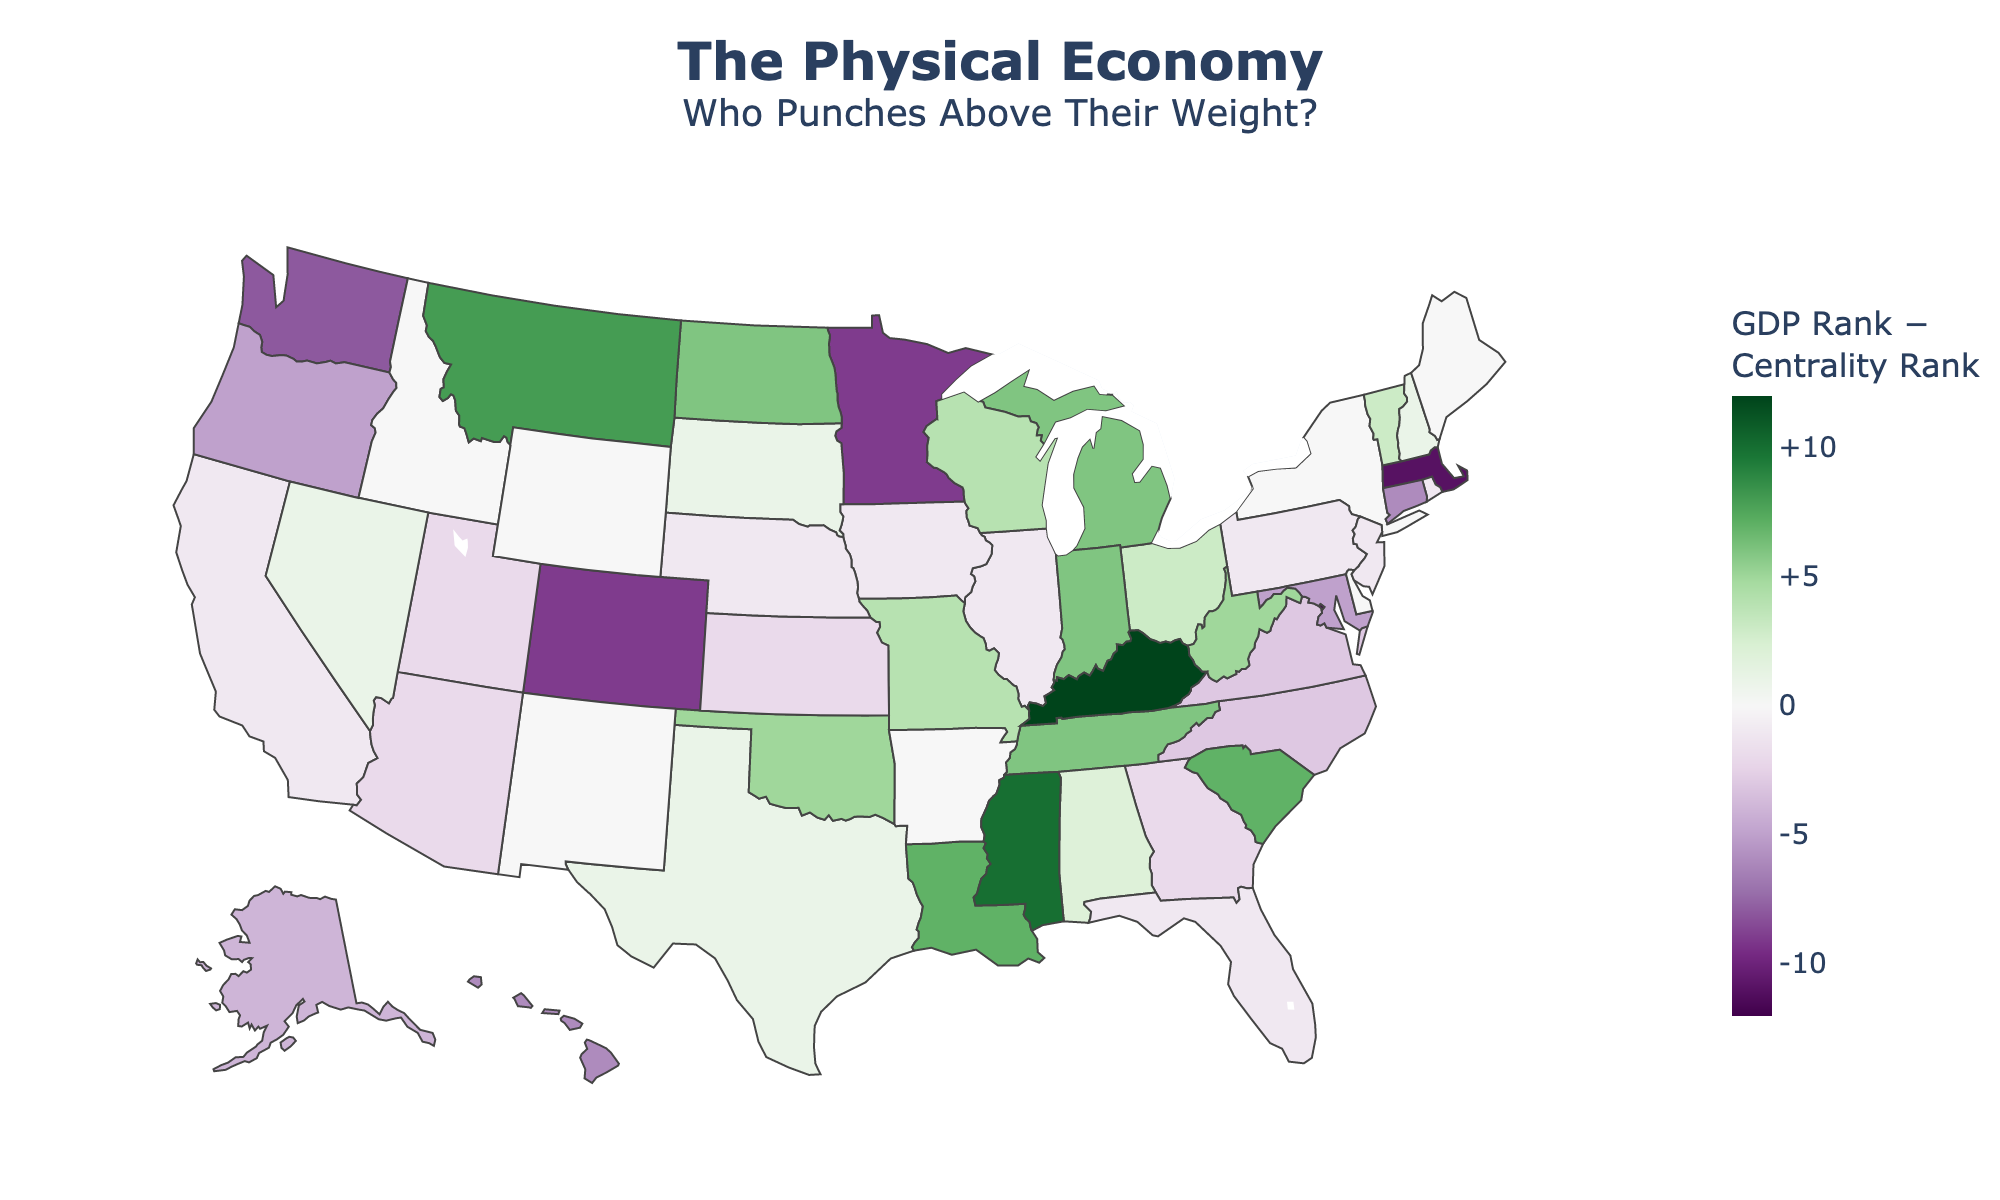
\includegraphics[width=\textwidth]{figures/marimo-physical-economy-divergence.png}
\caption[Geographic distribution of GDP-centrality divergence.]{Geographic distribution of GDP-centrality divergence. Green: states ranking higher in centrality than GDP predicts (e.g., KY +14, IN +6, TN +6). Purple: states ranking lower (e.g., WA -8, CO -9, MA -11).}
\label{fig:physical_economy}
\end{figure}

Table~\ref{tab:divergence} summarizes the extreme cases. The eight largest overperformers include six states east of the Mississippi; the five most significant underperformers are dominated by service and knowledge economies, with three ranking in the top 20 by GDP (MA, CO, WA). 

\begin{table}[ht]
\centering
\footnotesize
\caption[States with Extreme Divergence Between Economic Size and Network Position.]{States with Extreme Divergence Between Economic Size and Network Position. Positive $\Delta$ indicates structural overperformance relative to GDP; negative indicates underperformance. Norm.\ Rank shows position when centrality is divided by GDP.}
\label{tab:divergence}
\begin{tabular}{lcccc}
\hline
\textbf{State} & \textbf{GDP Rank} & \textbf{Eig.\ Rank} & \textbf{Rank $\Delta$} & \textbf{Norm.\ Rank} \\
\hline
\multicolumn{5}{l}{\textit{Structural Overperformers}} \\
KY & 28 & 14 & +14 & 2 \\
MS & 37 & 27 & +10 & 1 \\
MT & 49 & 41 & +8 & 6 \\
LA & 24 & 17 & +7 & 10 \\
SC & 26 & 19 & +7 & 4 \\
TN & 18 & 12 & +6 & 8 \\
MI & 14 & 8 & +6 & 13 \\
IN & 16 & 10 & +6 & 3 \\
\hline
\multicolumn{5}{l}{\textit{Structural Underperformers}} \\
DC & 34 & 49 & -15 & 48 \\
MA & 11 & 22 & -11 & 44 \\
MN & 17 & 26 & -9 & 38 \\
CO & 19 & 28 & -9 & 33 \\
WA & 13 & 21 & -8 & 41 \\
\hline
\end{tabular}
\end{table}


\clearpage
\section{International Integration Effects}
\label{sec:international}

How does boundary specification affect centrality rankings? This question (RQ2) measures how centrality rankings change when we treat U.S. commodity trade as the open system it actually is, rather than an artificially closed domestic network. We add international flows through a Rest of World (RoW) node and measure ranking stability. Table~\ref{tab:boundary_effects} summarizes differential boundary effects across measures.

\begin{table}[ht]
\centering
\caption{Boundary Sensitivity: a snapshot of how state centrality rankings change in the domestic vs. international networks.}
\label{tab:boundary_effects}
\begin{tabular}{lccccc}
\hline
\textbf{Measure} & \textbf{Spearman $\rho$} & \textbf{States} & \textbf{Top-5} & \textbf{Mean} & \textbf{Max} \\
                 &                          & \textbf{Changed} & \textbf{Overlap} & \textbf{$|\Delta|$} & \textbf{$|\Delta|$} \\
\hline
Betweenness   & 0.816 & 51/51 (100\%) & 60\%  & 5.3 & 7 \\
Eigenvector   & 0.982 & 43/51 (84\%) & 60\%  & 2.4 & 7 \\
Out-Degree    & 0.994 & 45/51 (88\%) & 100\% & 1.5 & 4 \\
\hline
\end{tabular}
\end{table}

\textbf{Betweenness} is the most sensitive to boundary specification ($\rho = 0.816$). International flows create new shortest paths through gateway states, redistributing bridging roles. Interior states like Ohio (7 to 14) and Pennsylvania (4 to 9) decline while coastal states like Washington (8 to 6) gain. \textbf{Eigenvector} remains more stable ($\rho = 0.982$) but still shifts. Washington jumps 6 ranks, Hawaii 7, as international connectivity reshapes which neighbors count as important. \textbf{Out-degree} is nearly unchanged
($\rho = 0.994$): the top-5 producers (CA, TX, IL, PA, OH) hold position regardless of boundary specification, because raw output volume does not depend on network routing. The more a centrality measure depends on global network structure, the more boundary specification seems to matter. 

The scatter plots and choropleth below make these patterns visible. Figure~\ref{fig:rank_betweenness} shows betweenness rank changes; eigenvector and out-degree scatter plots are in Appendix~\ref{appendix:rank_scatters}.

\begin{figure}[htbp]
\centering
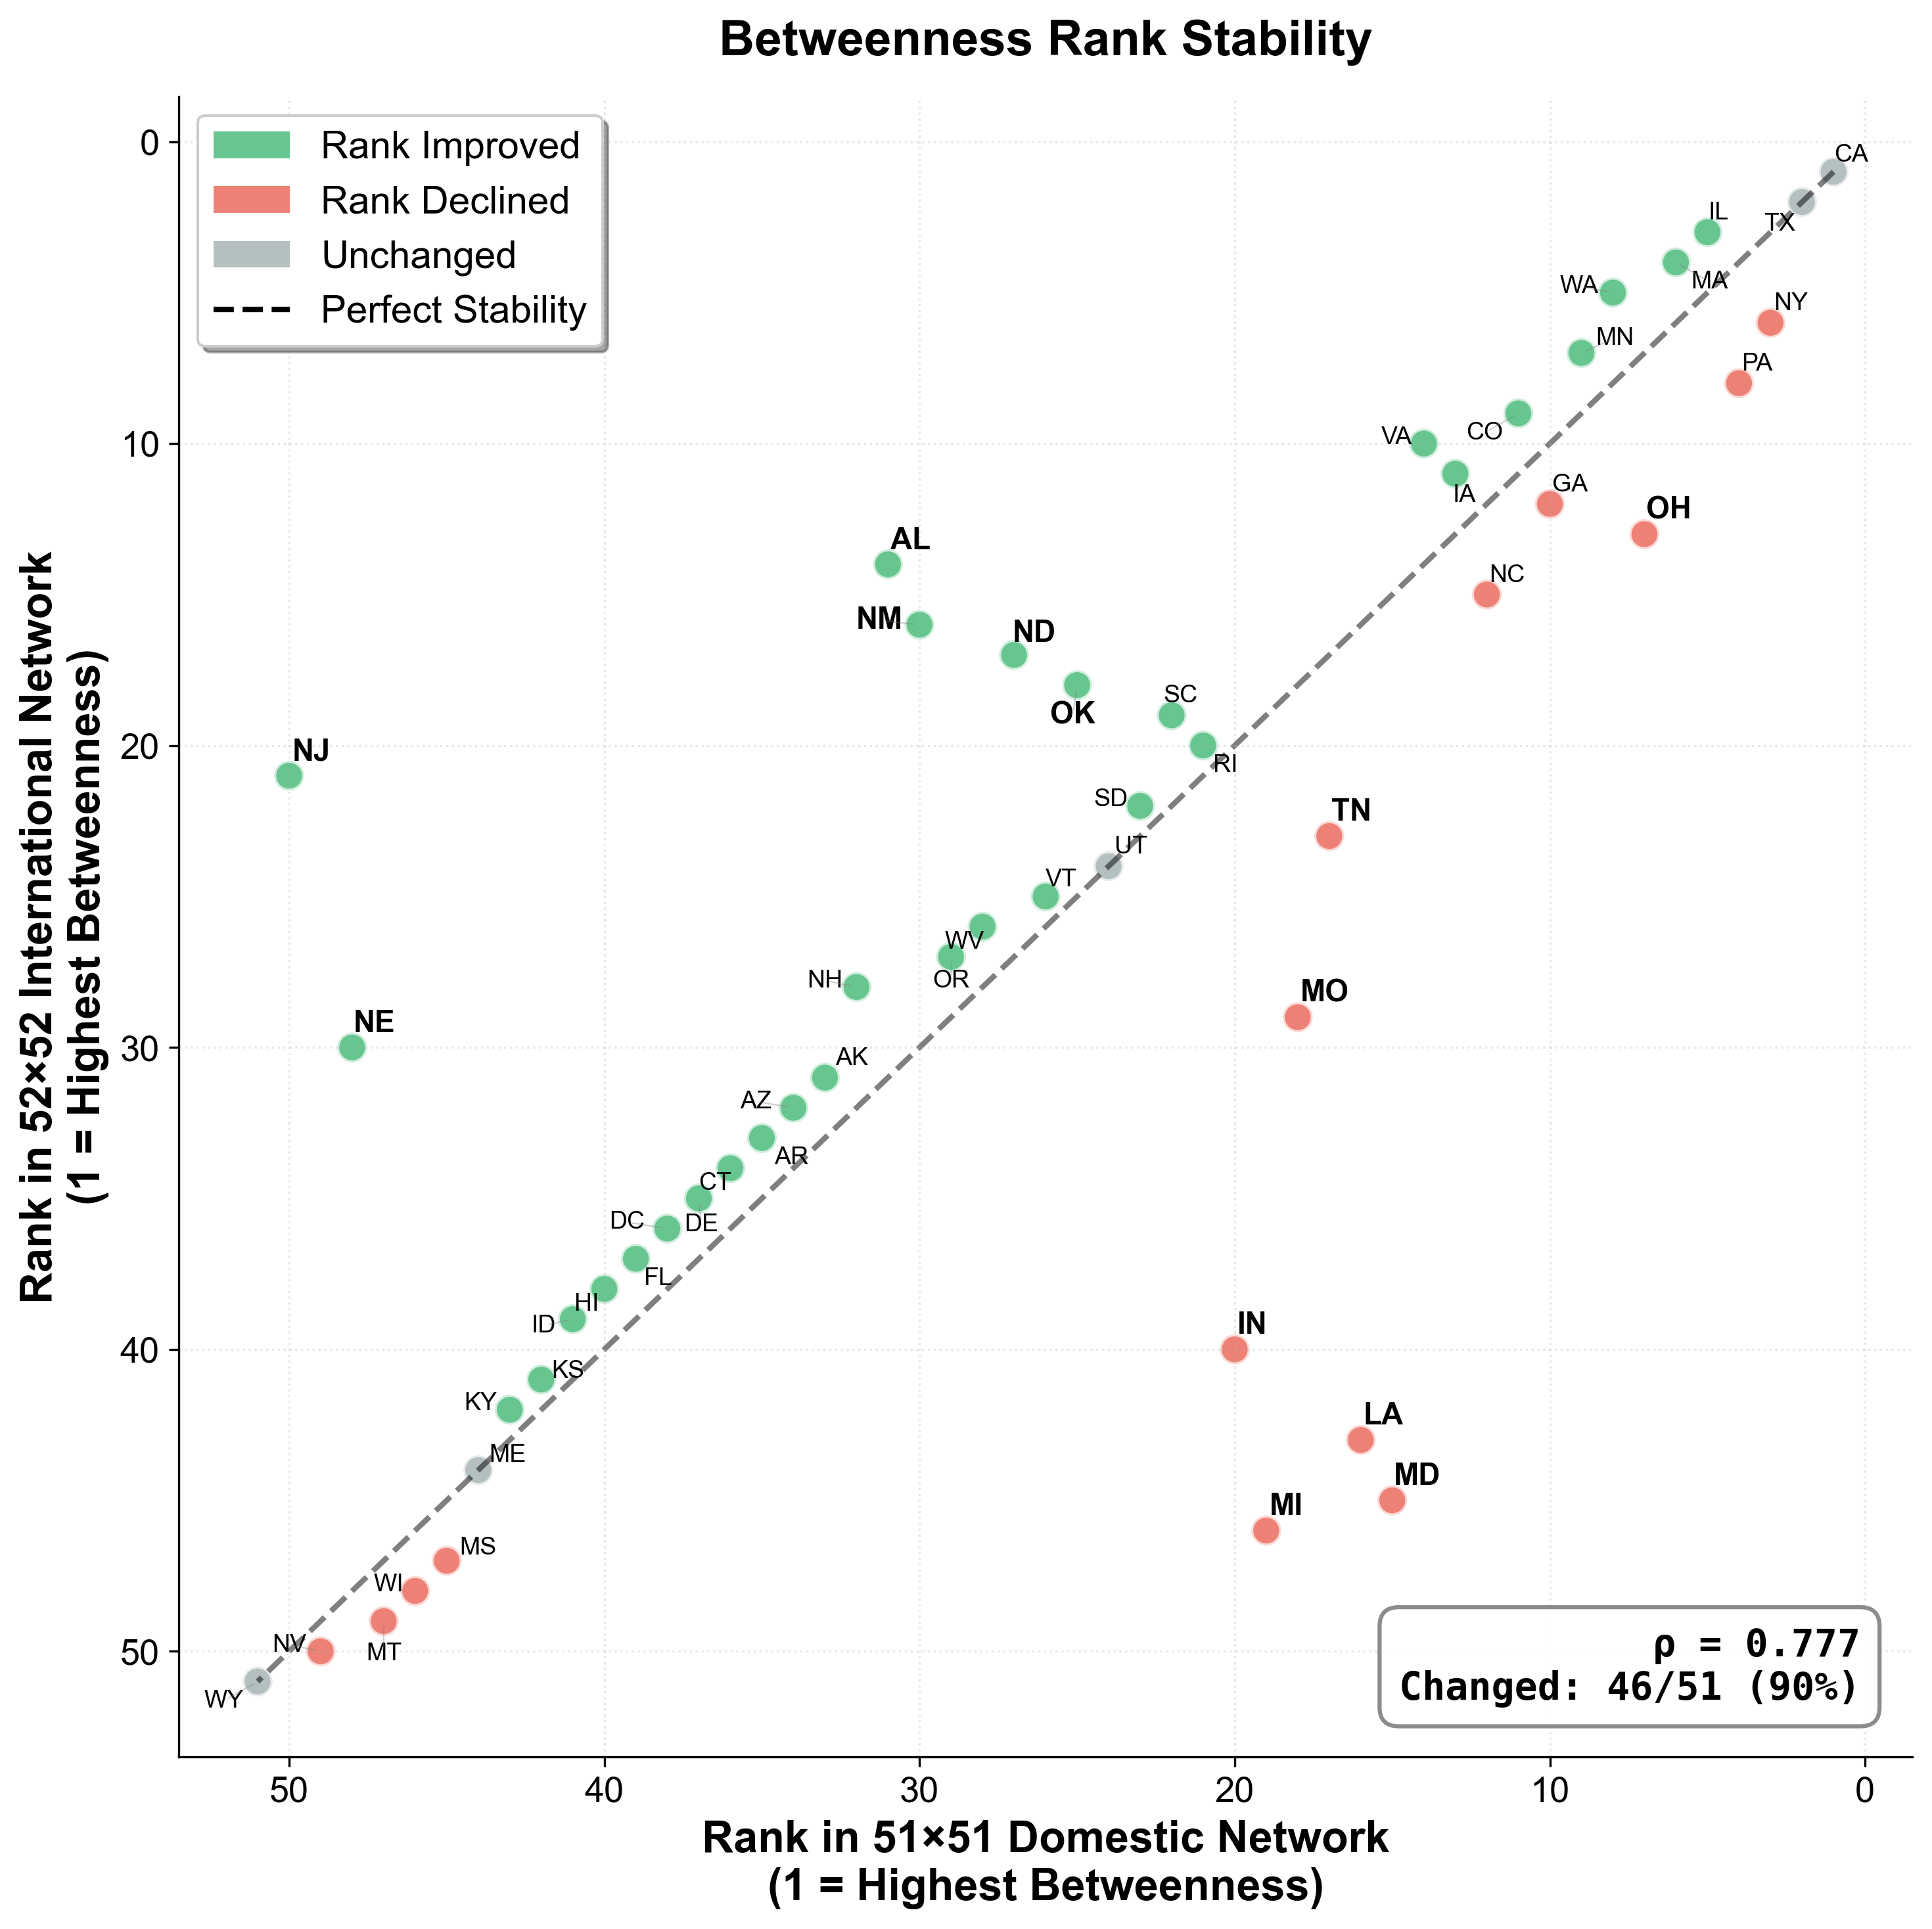
\includegraphics[width=\textwidth]{figures/rank_scatter_betweenness.png}
\caption[Betweenness rank changes between domestic and international networks.]{Betweenness rank changes between domestic and international networks. Points on diagonal indicate no rank change. Green: improved; red: declined.}
\label{fig:rank_betweenness}
\end{figure}

Figure~\ref{fig:rank_change_summary} summarizes the pattern: sensitivity increases with path dependence. Figure~\ref{fig:boundary_choropleth} maps the geographic distribution of eigenvector rank changes, revealing a spatial pattern in which coastal gateway states gain influence while interior bridge states lose it. 

\begin{figure}[htbp]
\centering
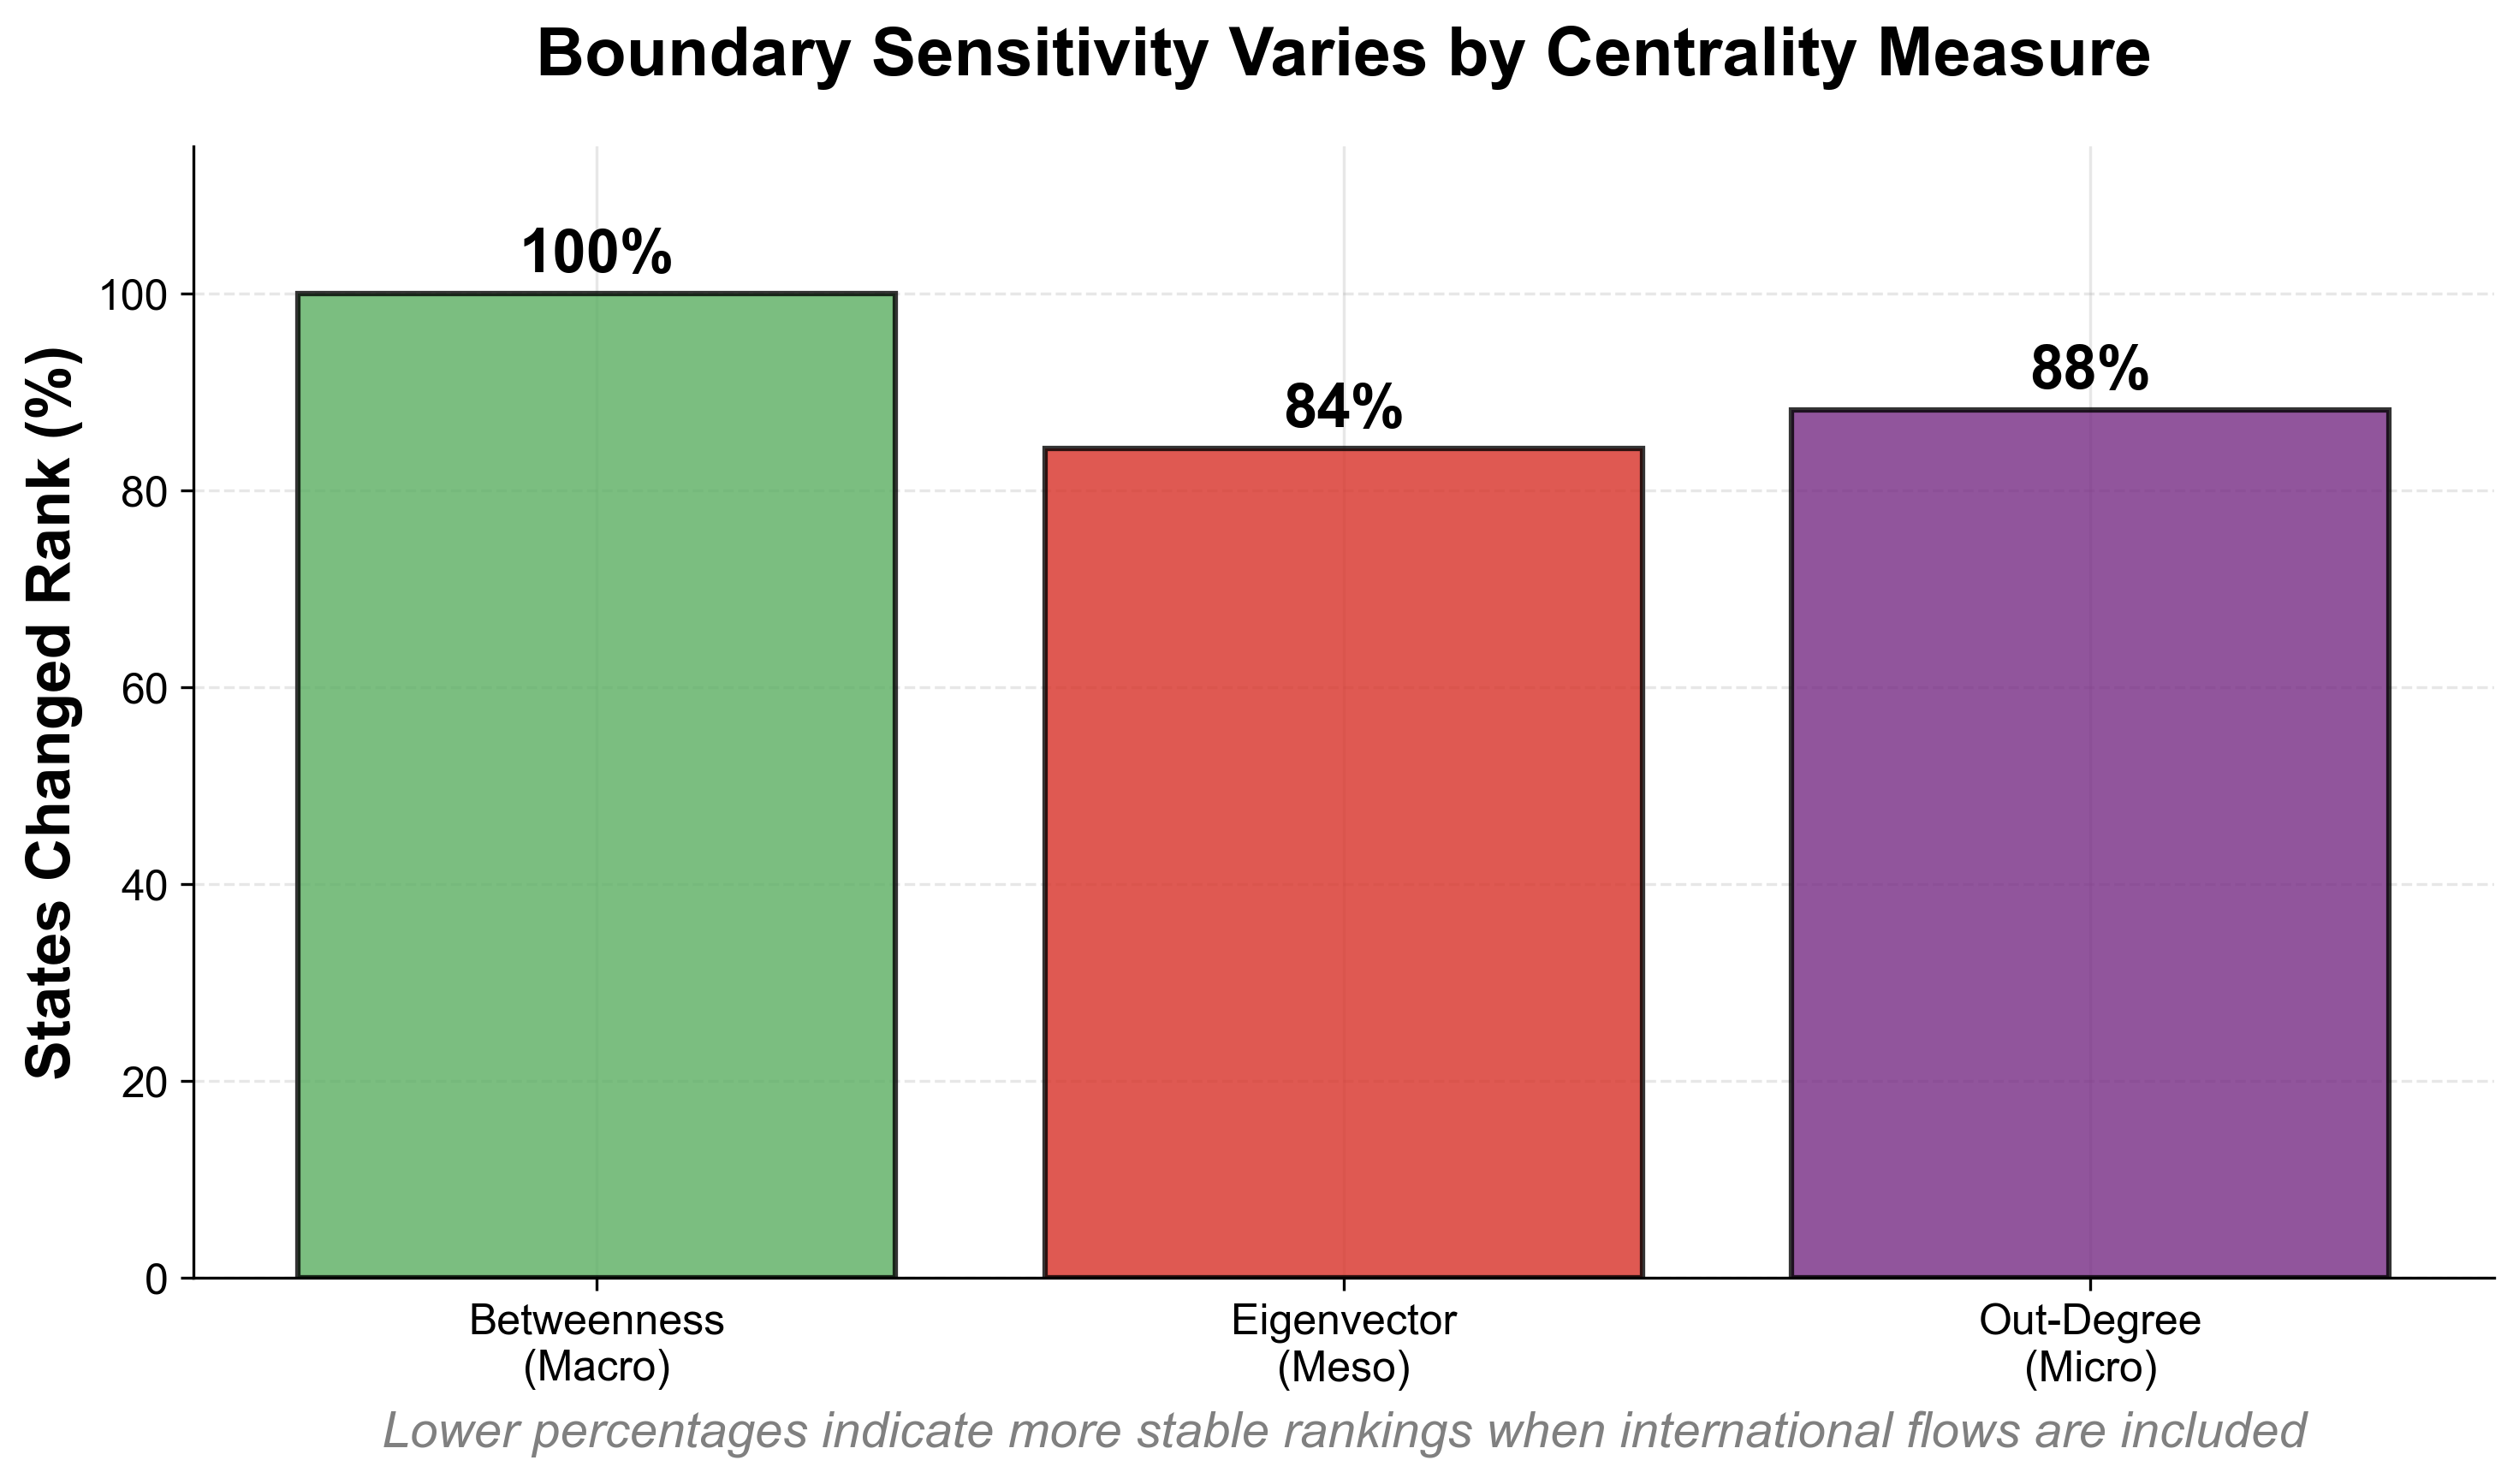
\includegraphics[width=\textwidth]{figures/boundary_sensitivity_summary.png}
\caption[Boundary sensitivity varies by measure type.]{Boundary sensitivity varies by measure type. Betweenness (path-based) shows highest sensitivity; out-degree (connection-based) shows highest stability.}
\label{fig:rank_change_summary}
\end{figure}

\begin{figure}[htbp]
\centering
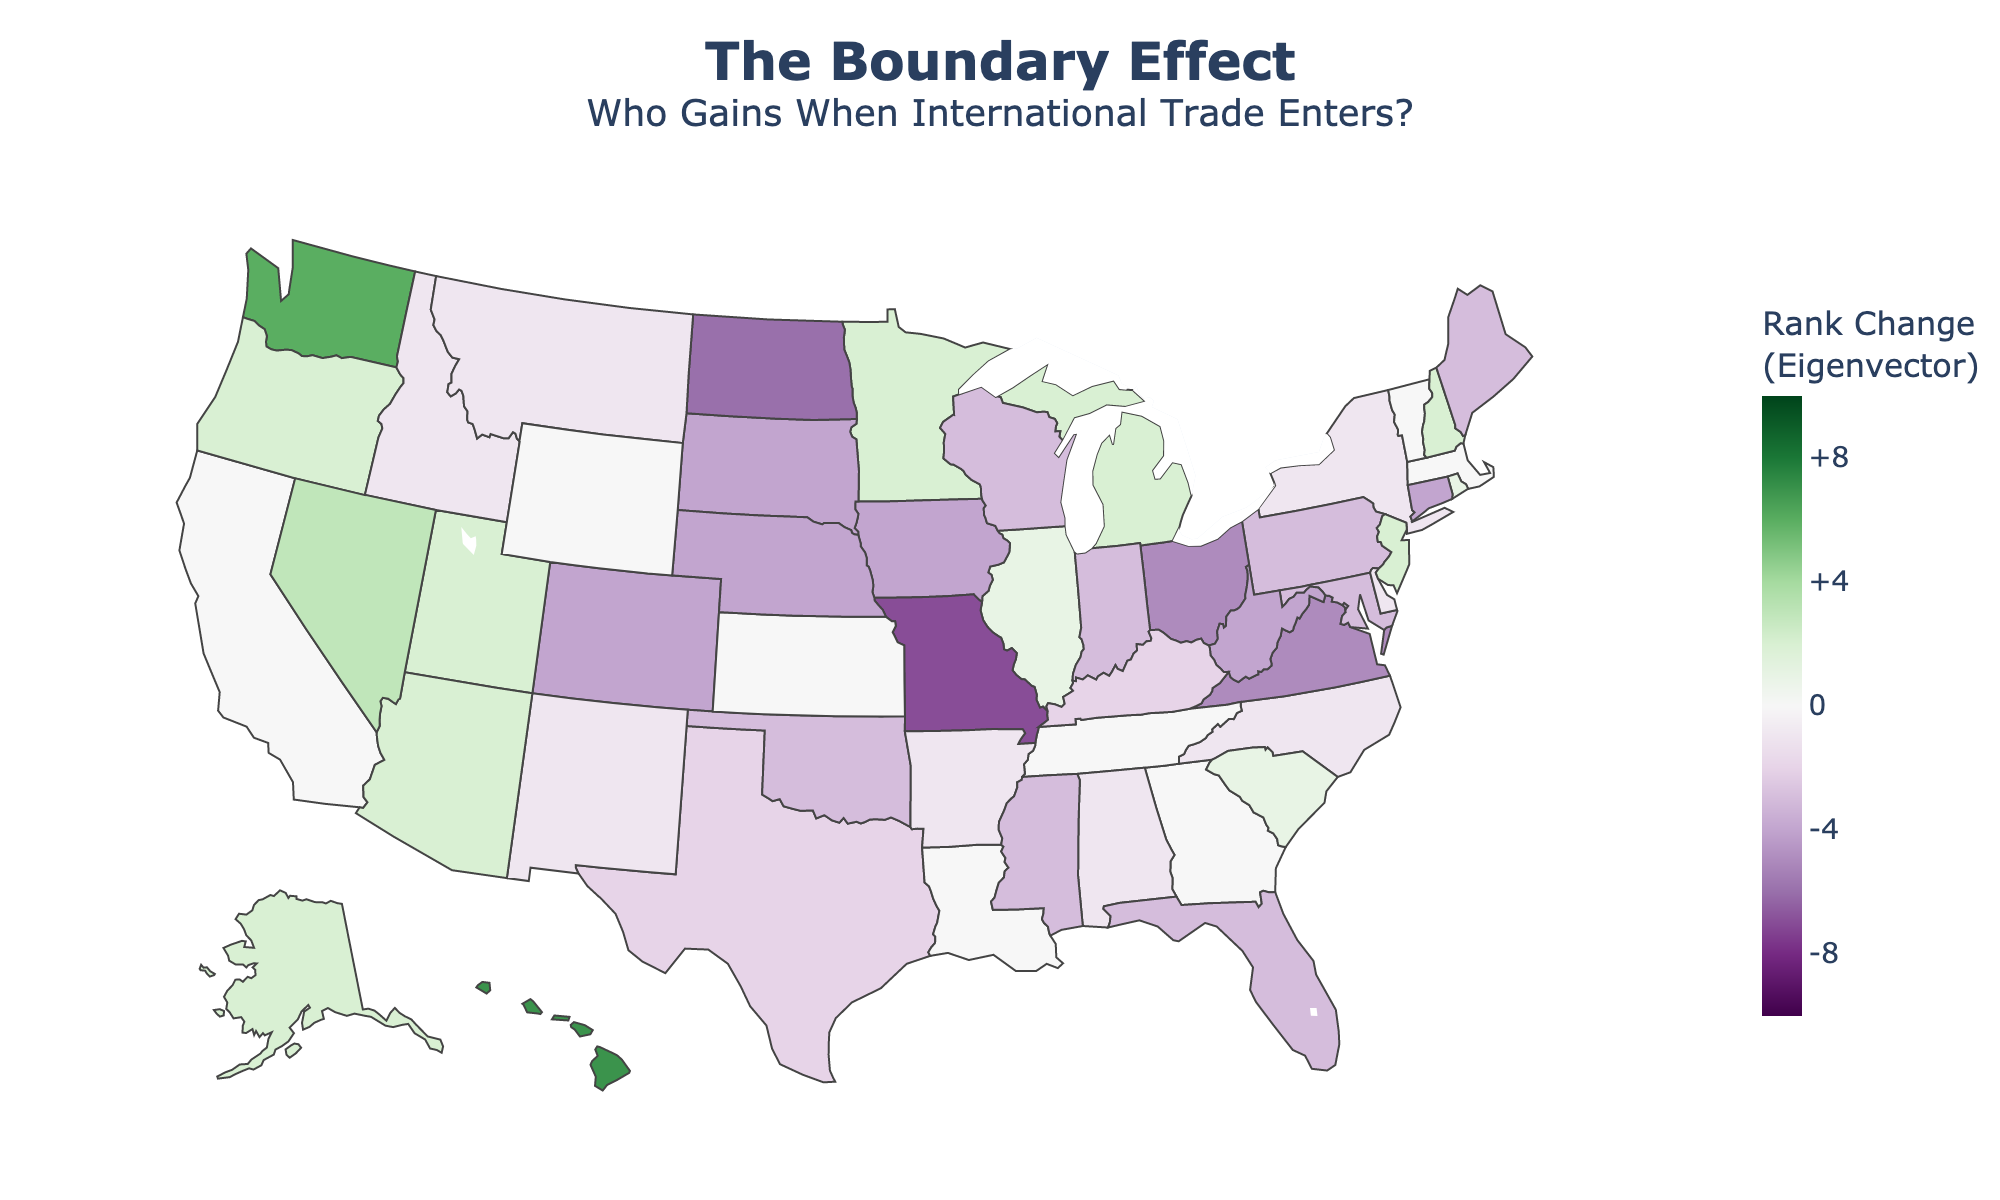
\includegraphics[width=\textwidth]{figures/marimo-boundary-effect.png}
\caption[Geographic distribution of eigenvector rank changes when international flows are added.]{Geographic distribution of eigenvector rank changes when international flows are added. Green: improved ranking; purple: declined.}
\label{fig:boundary_choropleth}
\end{figure}

\FloatBarrier
\chapter{Discussion}

\section{Network Position Does Not Equal Economic Size}

Our core finding is that nearly 40\% of states diverge by five or more ranks between GDP and eigenvector centrality. This provides a clear answer to \textbf{RQ1}: network analysis reveals structural information not captured by GDP alone.

The most striking pattern is that states with manufacturing, energy, and agricultural economies achieve network positions far exceeding their GDP rankings. Kentucky ranks 28th in GDP but 14th in eigenvector centrality. Mississippi ranks 37th in GDP but 27th in centrality. Indiana, Louisiana, Michigan, and Tennessee show similar patterns. These states are the backbone of the physical economy, structurally central to domestic commodity flows. Yet this importance is invisible in GDP-based economic discourse. GDP systematically undervalues states whose primary role is enabling production elsewhere.

Service-dominated economies show the mirror pattern. Massachusetts, Colorado, and Washington D.C. rank lower in the commodity network than their GDP predicts. This is expected. GDP captures value creation from software, financial services, and professional consulting that does not flow through physical goods. Their underperformance confirms we are measuring what we intend to measure: \emph{the structure of commodity trade}, not total economic output.

Industry composition data from the Bureau of Economic Analysis \cite{bea_gdp_state_2024} is consistent with both patterns. Overperforming states have manufacturing as their largest or second-largest sector, while underperforming states are dominated by finance, professional services, and technology.

The case of Florida and New Jersey reveals what GDP obscures. Both states rank high in GDP (4th and 8th respectively) but have zero betweenness centrality. They produce a great deal, but they are not trade corridors. No shortest path in the network runs through them. GDP cannot tell us this.

Each centrality measure correlates differently with GDP, and these differences matter. Eigenvector centrality correlates strongly ($\rho = 0.934$), tracking economic size. Out-degree correlates similarly ($\rho = 0.904$), tracking output capacity. Betweenness correlates only moderately ($\rho = 0.763$), capturing something distinct: structural brokerage position. By measuring which states lie on paths between other states, betweenness reveals a dimension of structural importance that aggregate output measures miss entirely. Betweenness is too concentrated to serve as a normalization baseline, as thirty-one states (61\%) have zero betweenness, reflecting the backbone structure of commodity flows through a small number of hub states. This concentration is itself a finding: most states participate in trade without serving as intermediaries. 

\section{The Domestic Network is Not the International Network}

Our second finding directly answers \textbf{RQ2}: adding the Rest of World node, transforming the network from closed domestic to open with international flows, significantly alters network structure. The three centrality measures respond differently to this boundary change. Betweenness is highly sensitive ($\rho = 0.816$), because path-based measures depend on network topology, which changes when adding the RoW node creates new shortest paths. Eigenvector is moderately sensitive ($\rho = 0.982$), as gateway states gain prestige through their RoW connection. Out-degree demonstrates high stability ($\rho = 0.994$), as adding international flows increases outbound capacity without reshuffling relative rankings. This differential sensitivity reveals what these measures actually capture: betweenness is topology-dependent, eigenvector is prestige-dependent, and out-degree is capacity-dependent.

Adding international flows causes network influence to shift from interior bridges to international gateways. Gateway states --- Washington (+6 eigenvector ranks), Hawaii (+7), New Jersey (+3) --- gain importance as their geographic access to international markets translates into network prestige. Interior states lose: Ohio (-5 eigenvector), Missouri (-7) --- domestic bridges are bypassed when gateways connect directly to Rest of World. Ohio's betweenness dropped 7 ranks as international routes circumvented the Midwest corridor.

These findings have methodological implications. Researchers should explicitly specify network boundaries when measuring structural power, as betweenness rankings depend critically on whether international trade is included.


\section{Betweenness Stability Under Filtration}

Segarra \& Ribeiro \cite{segarra_stability_2015} proved that betweenness centrality is mathematically discontinuous under standard computation, leading some researchers to avoid it in dense networks. Our filtration analysis shows this concern does not apply when proper weight inversion is used. All three centrality measures show perfect rank stability ($\rho = 1.000$) under 33\% edge removal. In this network, betweenness instability appears to be an artifact of incorrect weight treatment, not the inherent mathematical limitation identified by Segarra \& Ribeiro. With correct weight inversion, betweenness reliably identifies bridging positions even at 99.4\% network density.

\section{Broader Implications}

The Federal Reserve tracks dozens of economic indicators. All are statistical aggregates; none are derived from network models. This reflects a broader pattern: network science has proven powerful for economic analysis, but it has not been translated into accessible metrics for policymakers.

GDP dominates economic discourse because it is simple and intuitive. But simplicity obscures structural importance. Kentucky ranks 28th in GDP but 14th in eigenvector centrality. Its imports comprise 32.3\% of state GDP, the highest in the nation \cite{bea_gdp_state_2024}. The state's economy depends on and enables integrated supply chains, yet GDP metrics position it as a minor economic player. This pattern repeats across manufacturing states: structurally important but economically invisible.

We call this pattern \emph{Structural Undervaluation}. GDP ranks states by final output. Eigenvector centrality reveals their role in enabling output elsewhere. The disconnect between structural importance and economic recognition is real and quantifiable. Whether this contributes to political underrepresentation in economic policy is beyond our scope, but the measurement gap exists.

Supply chain resilience depends on structural position, not just economic size. A disruption to a high-betweenness state affects paths between other states. A disruption to a high-eigenvector state affects well-connected partners. Our boundary sensitivity analysis adds nuance: states identified as critical domestic bridges may be less essential when international supply chains are considered. Ohio ranks 7th in domestic betweenness but drops to 14th when international flows are included. Its bridging role may be partially redundant with international gateways.

Policy targeting supply chain resilience should match boundary specification to threat model. Domestic disruptions (natural disasters, infrastructure failure) may require domestic-only analysis. Trade policy disruptions may require internationally-integrated analysis.


\section{Limitations}

This analysis measures economic centrality through commodity trade flows only. Several constraints limit interpretation.

First, commodity flows exclude services, financial flows, and information exchange. A state's structural importance encompasses dimensions beyond physical goods trade. Second, our 2017 snapshot cannot capture temporal dynamics. Supply chain restructuring, trade policy changes, and economic shocks alter network structure over time. Third, state-level analysis masks within-state variation. California's ports and Central Valley play different structural roles; our analysis cannot distinguish them. Fourth, our Rest of World node treats all international partners as equivalent, obscuring heterogeneous relationships with different trading partners. Chapter~\ref{sec:future_work} addresses each of these constraints and proposes additional extensions.


\FloatBarrier
\chapter{Future Work}
\label{sec:future_work}

This analysis establishes network centrality as a valid approach for measuring structural economic power in commodity trade. However, several extensions are needed to strengthen the framework.

\section{Methodological Foundations}
\subsection{Pre-Analysis Normalization}

Our analysis applies normalization after centrality computation --- comparing un-normalized rankings against GDP rankings. This raises the question of whether the nearly 40\% divergence pattern reflects a genuine structural feature, or an artifact of this specific approach. To investigate this, we ran pre-analysis normalization of edge weights, dividing every edge weight by the sender's GDP \textbf{before} computing centrality, and then recomputing all three centralities on the normalized network. We compared pre-normalized centrality rankings vs. post-normalized ones via Spearman correlation and found that Eigenvector rankings barely changed ($\rho = 0.980$). Betweenness rankings changed moderately ($\rho = 0.601$), and out-degree rankings changed significantly ($\rho = 0.375$). While more extensive exploration of various approaches to pre-normalization is warranted, these results do suggest that the divergence pattern is a structural feature of the network, not an artifact of economic scale.  


\subsection{Filtration Sweep}

Our analysis tested a single filtration threshold at 33\%, the maximum filtration level before the network loses its strongly connected component. Sweeping filtration from the complete network in 5\% increments would map centrality stability across the full density range, revealing where rankings first destabilize and where the network begins to fragment. This is important because thresholds that produce identical connected components might yield meaningfully different centrality hierarchies. A ranking that holds across a wide density range would carry more interpretive weight than one that emerges only at a narrow threshold. 

\section{Analytical Extensions}
\subsection{Geographic Predictors}
Network centrality captures structural position within commodity flows, but does not distinguish whether that position is driven by economic activity or physical geography. Testing geographic features; spatial position, interior waterway access, and coastal exposure as predictors of network centrality would reveal whether geography independently explains network centrality, separating structural role from locational advantage. States that are structurally central despite unfavorable geography would tell a different story than those whose centrality is largely a function of where they sit on a map. 

\subsection{Commodity Disaggregation}
Aggregating all SCTG categories into a single network is appropriate for an initial analysis, but it obscures which goods classes drive centrality patterns. Commodity-level disaggregation could reveal whether the structural undervaluation we identified is a general feature of interstate trade, or concentrates in specific sectors: agricultural goods, manufactured products, or raw materials. A sector-specific pattern would point towards industry-level explanations, while a uniform one would strengthen the case for structural position as the dominant factor. 

\subsection{Temporal Analysis}

Our analysis only captures a single snapshot in time, limited to the 2017 CFS release. Applying this framework to the 2012 survey would provide a clean pre-period comparison, revealing whether structural positions were stable across years of relative continuity. The 2022 release raises a different and more compelling question: which states' structural positions shifted in response to COVID-era supply chain disruption, and which proved resilient? Jang \& Yang discarded post-COVID data in their longitudinal approach to avoid conflating disruption with structural change \cite{jang_measuring_2023}, but that conflation is precisely what a disruption-focused analysis would shed light on. Together, the three surveys would span a full arc: pre-period baseline, stable-period snapshot, and disruption response. 

\subsection{Rest of World Disaggregation}
We chose to aggregate all international trade partners into a single ``Rest of World'' node to reduce complexity for our initial analysis, rather than trying to identify state-level trade with individual countries. While the FAF5 does not provide granular detail about trade with every country, it does have foreign region codes that represent regional aggregates (Europe, Africa, Eastern Asia, etc.). Full disaggregation to individual trading partners would provide finer resolution, but would also require integration of other data sources. Disaggregating into these regional nodes would reveal whether the betweenness sensitivity we documented ($\rho = 0.816$) concentrates on a few dominant trading regions or distributes broadly across all international partnerships. 



\section{Theoretical Development}
\subsection{Conservation Constraints}

Whether commodity flows satisfy conservation constraints at state nodes is an open theoretical question. If inflows and outflows roughly balance, then imbalances become interpretable signals of accumulation or transformation. If they do not, then centrality measures require different theoretical grounding. Spatial price equilibrium models and ecological throughflow analysis have formalized such nodal balance conditions in economic and biological flow networks \cite{takayama_spatial_1971, hannon_structure_1973}. Applying equivalent tests to the CFS network would clarify how to interpret the flow asymmetries our analysis surfaces. 

\subsection{Multiplex Framework}

Our operationalization captures one specific channel of structural position: commodity flows as measured by the CFS. Financial flows, service connections, and political influence each operate through distinct relational structures. Interstate bank lending and venture capital deployment would capture financial power. Origin-destination air travel, interstate commuting matrices, and patent citation networks would capture service flows. FEC campaign finance data, where donor networks reveal which states fund electoral activity beyond their own borders, would capture political influence. A multiplex network framework, in which each flow type constitutes a separate layer over the same 51-state node set, would allow researchers to identify states that are structurally central across multiple dimensions simultaneously, moving toward a comprehensive structural power index for U.S. states. For relationships that are inherently group-level rather than pairwise, such as multi-state supply chains, hypergraph representations offer a further theoretical extension worth considering. 

Beyond multiplexity, economic networks also exhibit \emph{hierarchical structure}: states contain metropolitan areas, which contain firms, each generating trade at different scales~\cite{simon_architecture_1962}. Recent multiresolution analysis of international trade networks has shown that hierarchical community structure, in the form of regional blocs that persist across resolution levels, is a key feature of trade topology~\cite{cho_multiresolution_2023}. Extending the present single-scale state-level analysis to a hierarchical decomposition that captures these nested scales is another natural direction for future work. Constructing such an index remains an open problem; the framework developed here provides the single-layer foundation on which it would rest. Developing these extensions would require interdisciplinary collaboration --- trade economists, regional scientists, political scientists, and network methodologists --- to strengthen normalization choices and ground structural findings in domain-specific interpretation.

This analysis has produced a working research artifact: an interactive visualization of the interstate commodity trade network, publicly deployed and available at \url{https://us-trade.plotly.app/}. The tool supports commodity-level filtering across all SCTG codes, a boundary sensitivity toggle that switches between domestic and international network specifications with live rank-change indicators, a filtration slider for stability analysis, and a rankings table with GDP divergence coloring that makes the structural undervaluation finding immediately visible. A full implementation would extend these capabilities to support multi-year comparison and commodity-level centrality analysis across the full SCTG taxonomy.


\FloatBarrier
\chapter{Conclusion}

It has been 92 years since Kuznets warned Congress that GDP cannot measure welfare. 89 years since Hayek called for ``topological'' approaches to economics, and 52 since he urged economists to shift their focus towards the prediction of general patterns in complex social systems. 78 since Weaver demonstrated why statistical aggregates cannot describe organized complexity. Deaton's 2024 lamentation that professional economists have failed to analyze power is a symptom of a deeper issue: mainstream economics has not adopted the methodologies needed to analyze power systemically. In 2026, the Federal Reserve tracks dozens of aggregate indicators and zero relational ones. This paper demonstrates that network science provides exactly the analytical framework these scholars called for. Given that the tools exist, the gap is not technical, it is institutional. 

We have shown that network centrality captures structural dimensions that GDP misses. Nearly 40\% of states demonstrate significant divergence between GDP and eigenvector centrality rankings, a pattern that tracks industry composition data from the Bureau of Economic Analysis. Service-dominated economies show the expected mirror pattern, confirming the framework measures commodity trade structure rather than total economic output. 

Betweenness centrality remains stable under graph filtration in our network when proper weight treatment is applied, extending the usable toolkit for dense economic networks despite prior instability concerns \cite{segarra_stability_2015}. Boundary specification produces measure-dependent effects; betweenness is highly sensitive to international inclusion while eigenvector and out-degree remain stable. This means analysts must match network boundaries to the question under consideration. 


These findings have immediate practical relevance. As governments and corporations invest hundreds of billions of dollars in data center infrastructure to support artificial intelligence, questions of structural economic power are becoming tangible. Seven of the eight states this framework identifies as structurally undervalued are now attracting major AI infrastructure investment --- collectively over \$170 billion announced since 2024~\cite{xai_mississippi_2026, amazon_mississippi_2025, compass_mississippi_2025, hut8_louisiana_2025, amazon_louisiana_2025}. This investment is driven by the same physical infrastructure factors that generate high network centrality: cheap energy, water access, grid capacity, and logistics corridors. The overlap is consistent with the structural features the framework captures. The model was not designed to predict data center investment, and the investment boom occurred after the analysis period. Mississippi, which ranks 37th in GDP but holds the highest GDP-normalized centrality in the nation, is receiving approximately \$49 billion in data center commitments. While tax incentive packages have played a role, states could credibly offer such incentives in part because they possessed the structural capacity to back them up. Montana, the eighth state, shows early-stage interest but an unproven pipeline --- an honest limit of the framework's reach. 

Adam Smith spoke of political economy, never economics, because he understood that political and economic systems cannot be analyzed as disjointed entities --- they are deeply intertwined \cite{smith_wealth_1776}. This separation is why economists struggle with power analysis, as Deaton has noted. Network science, combined with a reunified political economy, can offer sharper analytical tools than either economics or political science provides alone. Measuring structural position as a proxy for power, as we have done, is a small step towards more comprehensive measures that might inform a systems-theoretic political economy. 

Measurement shapes understanding, and understanding shapes politics. If states are structurally essential but economically invisible, this has implications for scientific analysis, civic discourse, and the everyday lives of citizens. If the patterns documented here prove robust across additional economic domains, political economists will need to reckon with what it means for states to be essential but invisible.

Network science insights have not yet reached the general public. For these findings to have impact beyond the halls of academia, citizens and policymakers will need accessible tools --- just as they rely on statistics from the Bureau of Labor Statistics and the Federal Reserve. This contribution should not be seen solely as academic; it is a prototype for open public infrastructure. We have built an interactive visualization that allows users to explore structural position across commodity categories, toggle boundary specifications and compare centrality with GDP rankings. The PNNL Data Center Atlas \cite{noauthor_im3pnnlgovdatacenter-atlas_nodate} offers a federal precedent, mapping data center facilities and their infrastructure dependencies as a publicly accessible tool. Building the equivalent for interstate trade --- a public dashboard showing structural position, not just GDP --- would serve citizens, entrepreneurs, and policymakers. 

Just as Kuznets sought to compress complex statistics into digestible form, modern researchers have the opportunity to develop new relational metrics in collaboration with political economists. The tools to reveal relational importance --- not just economic size --- should be public.



% Configure URL breaking
\Urlmuskip=0mu plus 1mu




\FloatBarrier
\appendix

\chapter{Formal System Definition}
\label{appendix:formal_system}

Following Klir's systems formalism \cite{klir_facets_2001}, we can define the U.S. interstate commerce network as a structured system $S = (T,
R)$ where $T$ represents thinghood (the measurable dimensions we track) and $R$ represents systemhood (the relations between those dimensions).

The thinghood $T$ consists of:
\begin{itemize}
  \item $V$ -- The set of nodes: 50 U.S. states plus DC for the domestic network, or 52 nodes including Rest of World for the international-inclusive network
  \item $E \subseteq V \times V$ -- Directed edges representing commodity flows between states
  \item $W: E \to \mathbb{R}^+$ -- Weight function mapping each flow to its survey-adjusted trade value
  \item $C$ -- Commodity types following SCTG classifications (aggregated in this analysis)
  \item $B \in \{\text{domestic}, \text{international}\}$ -- Boundary specification choice
\end{itemize}

The systemhood $R$ defines how these dimensions relate:
\begin{itemize}
  \item $R_{\text{flow}}: V \times V \to \mathbb{R}^+ \cup \{0\}$ -- Trade flow relation where $R_{\text{flow}}(s_i, s_j)$ equals the weight of edge $(s_i, s_j)$ if it exists, zero otherwise
  \item $R_{\text{boundary}}: B \times V \to \{0, 1\}$ -- Function determining which nodes are included based on boundary choice (e.g., $R_{\text{boundary}}(\text{domestic}, \text{RoW}) = 0$, $R_{\text{boundary}}(\text{international}, \text{RoW}) = 1$)
  \item $R_{\text{centrality}}: V \to \mathbb{R}^3$ -- Mapping from nodes to their betweenness, eigenvector, and out-degree centrality scores
\end{itemize}

Together, $(V, E, W)$ defines a weighted directed graph where edge directionality captures trade flow orientation and edge weights preserve economic magnitude. The $|V| \times |V|$ adjacency matrix representation has 51$\times$51 entries for the domestic network ($|V|=51$) and 52$\times$52 entries for the international-inclusive network ($|V|=52$). This formalism lets us frame these networks as different projections of the same underlying system, distinguished only by boundary specification $B$. Our comparative analysis then becomes a study of how centrality rankings respond to this projection choice.



\chapter{Top Bilateral Trade Flows}
\label{appendix:edge_list}

Table~\ref{tab:top_edges} presents the 50 largest bilateral commodity flows in the 51$\times$51 domestic network. The complete edge list (2,534 flows) is available in supplemental materials.

\begin{table}[ht]
\centering
\footnotesize
\caption{Top 50 Bilateral Trade Flows by Value (51$\times$51 Domestic Network)}
\label{tab:top_edges}
\begin{tabular}{llr}
\hline
\textbf{Origin} & \textbf{Dest} & \textbf{Value (\$B)} \\
\hline
NJ & NY & 78.0 \\
CA & TX & 69.7 \\
PA & NY & 65.2 \\
PA & NJ & 58.4 \\
GA & FL & 57.2 \\
IL & IN & 55.4 \\
NY & NJ & 50.6 \\
IL & WI & 48.0 \\
NJ & PA & 47.5 \\
TX & CA & 46.2 \\
OH & MI & 41.4 \\
TX & LA & 38.6 \\
CA & FL & 38.5 \\
TX & OK & 37.8 \\
CT & NY & 37.7 \\
CA & AZ & 37.1 \\
WI & IL & 37.0 \\
IN & OH & 36.1 \\
LA & TX & 35.3 \\
IL & MI & 34.9 \\
IN & MI & 34.8 \\
PA & OH & 34.6 \\
OH & IN & 34.1 \\
TN & GA & 33.5 \\
CA & WA & 32.9 \\
IN & IL & 32.6 \\
CA & OH & 32.2 \\
NY & PA & 32.1 \\
MI & OH & 31.3 \\
CA & NV & 31.3 \\
OH & PA & 30.5 \\
NC & SC & 30.2 \\
OR & WA & 29.5 \\
AL & GA & 29.0 \\
IL & TX & 29.0 \\
AZ & CA & 28.8 \\
MA & NY & 28.5 \\
WA & OR & 28.2 \\
MI & TX & 27.5 \\
OH & IL & 27.2 \\
MI & IL & 26.6 \\
SC & GA & 26.0 \\
IL & OH & 25.8 \\
OK & TX & 25.5 \\
CA & NY & 24.8 \\
IL & CA & 24.3 \\
GA & NC & 24.2 \\
GA & TN & 23.7 \\
CA & OR & 23.6 \\
NY & CA & 23.3 \\
\hline
\end{tabular}
\end{table}

\FloatBarrier

\chapter{Centrality vs.\ Control Variable Scatter Plots}
\label{appendix:scatters}

Figures~\ref{fig:gdp_betweenness_scatter}--\ref{fig:gdp_population_scatter} present scatter plots for all centrality--control combinations. Each plot compares a control variable rank (GDP or population) against a centrality measure rank, with Spearman $\rho$ annotated. These seven plots provide a complete picture of how economic size and population relate to structural position across all three centrality levels. Table~\ref{tab:rho_correlations} summarizes the Spearman correlations for all six centrality--control combinations.

\begin{figure}[ht]
\centering
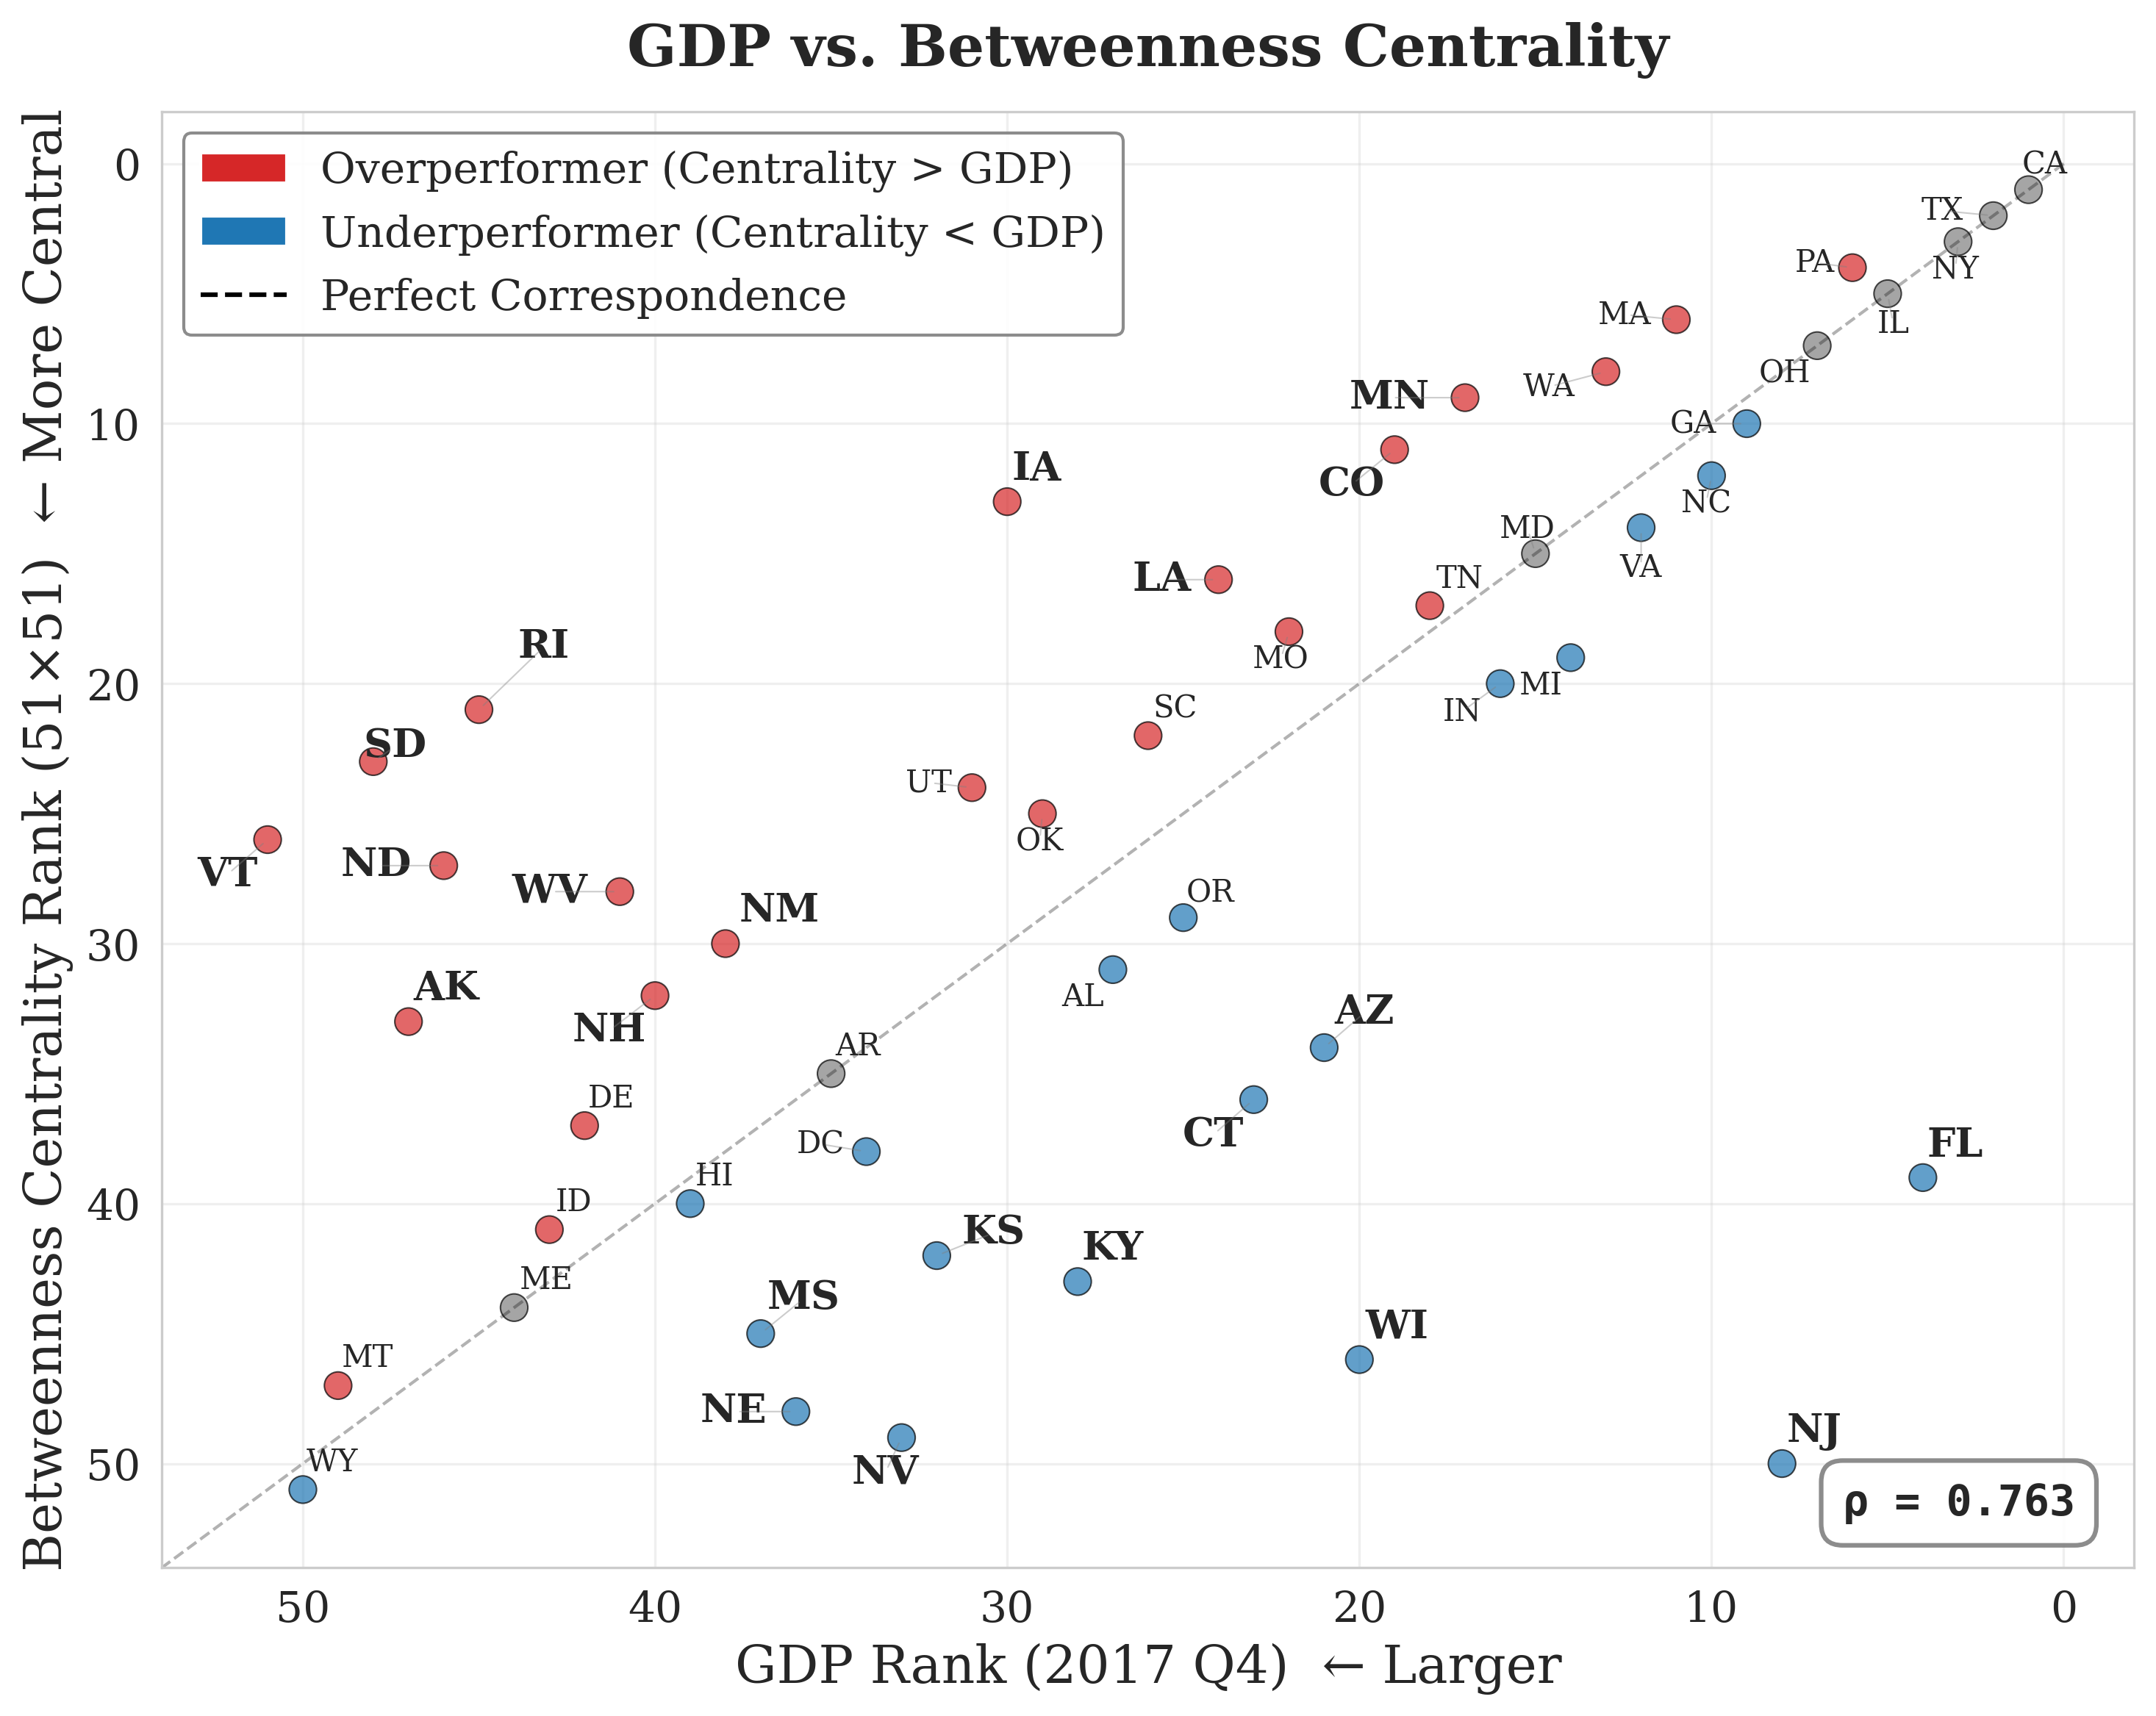
\includegraphics[width=\textwidth]{figures/gdp_vs_betweenness_scatter.png}
\caption[GDP rank vs.\ betweenness centrality rank ($\rho = 0.763$).]{GDP rank vs.\ betweenness centrality rank ($\rho = 0.763$). The moderate correlation reflects betweenness measuring structural brokerage rather than economic size. Thirty-one states share zero betweenness (tied ranks at right).}
\label{fig:gdp_betweenness_scatter}
\end{figure}

\begin{figure}[ht]
\centering
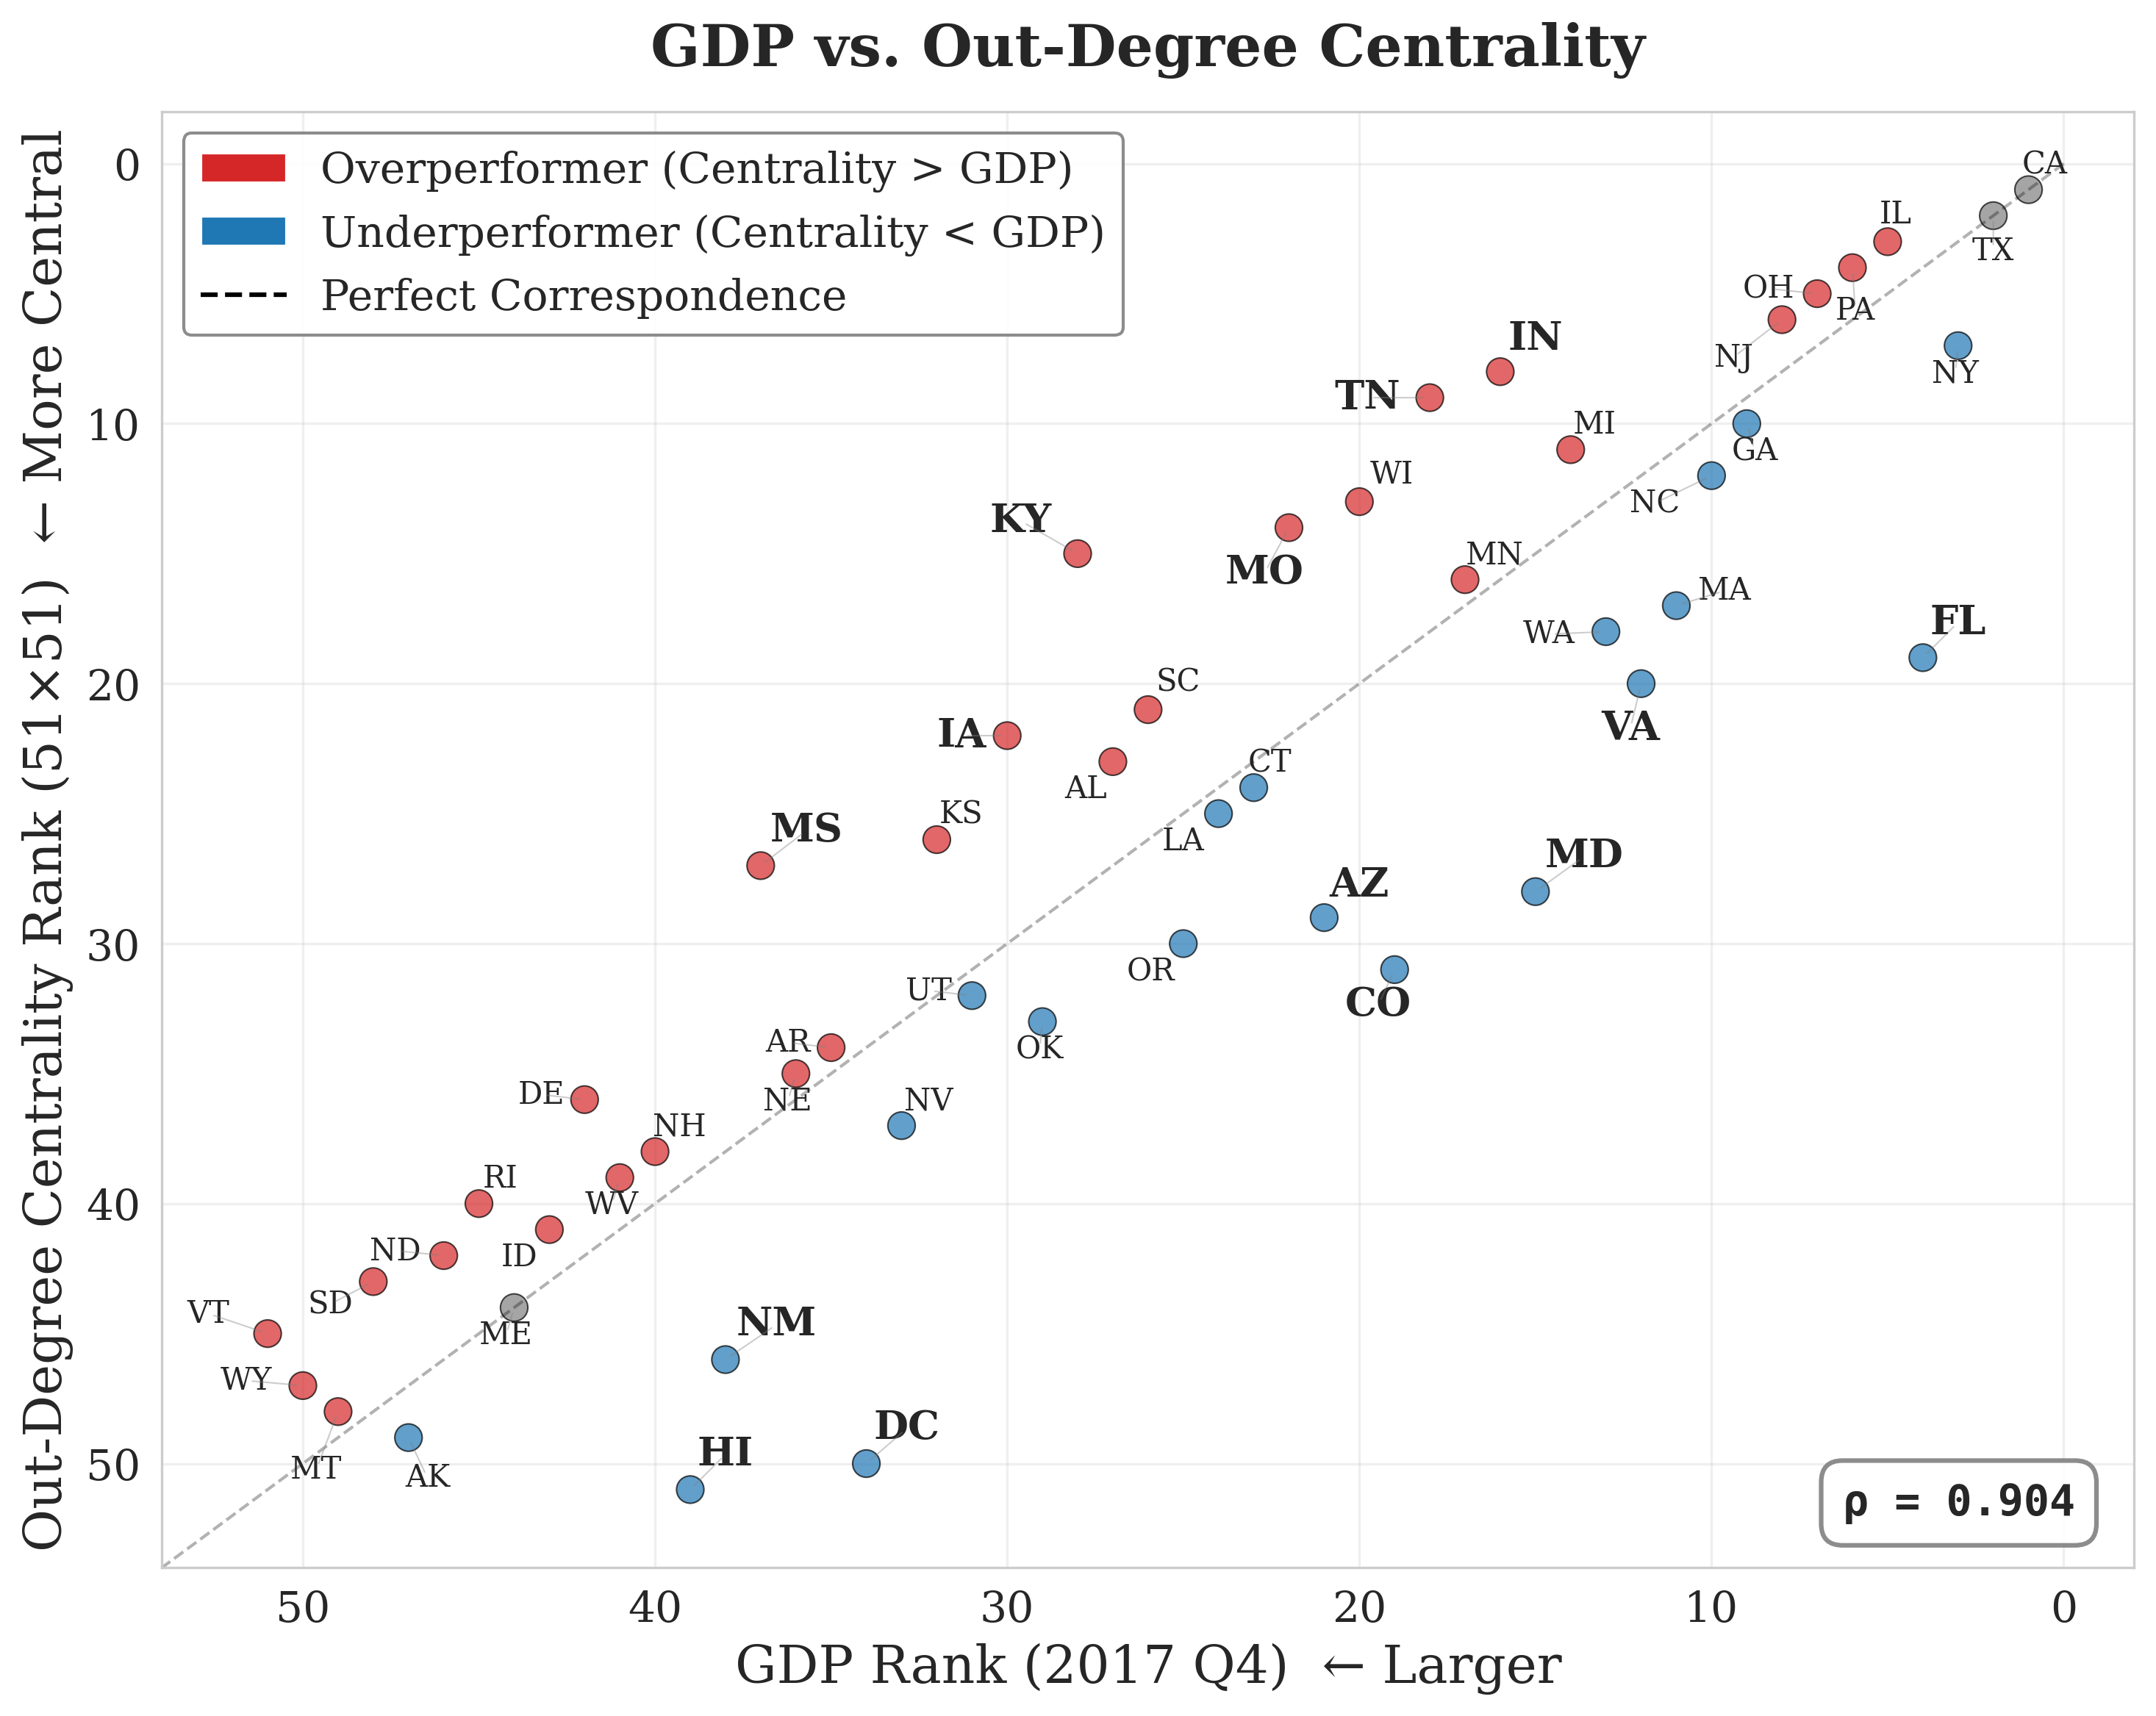
\includegraphics[width=\textwidth]{figures/gdp_vs_out_degree_scatter.png}
\caption[GDP rank vs.\ weighted out-degree centrality rank ($\rho = 0.904$).]{GDP rank vs.\ weighted out-degree centrality rank ($\rho = 0.904$). Strong correlation indicates total outbound trade volume tracks economic size closely.}
\label{fig:gdp_outdegree_scatter}
\end{figure}

\begin{figure}[ht]
\centering
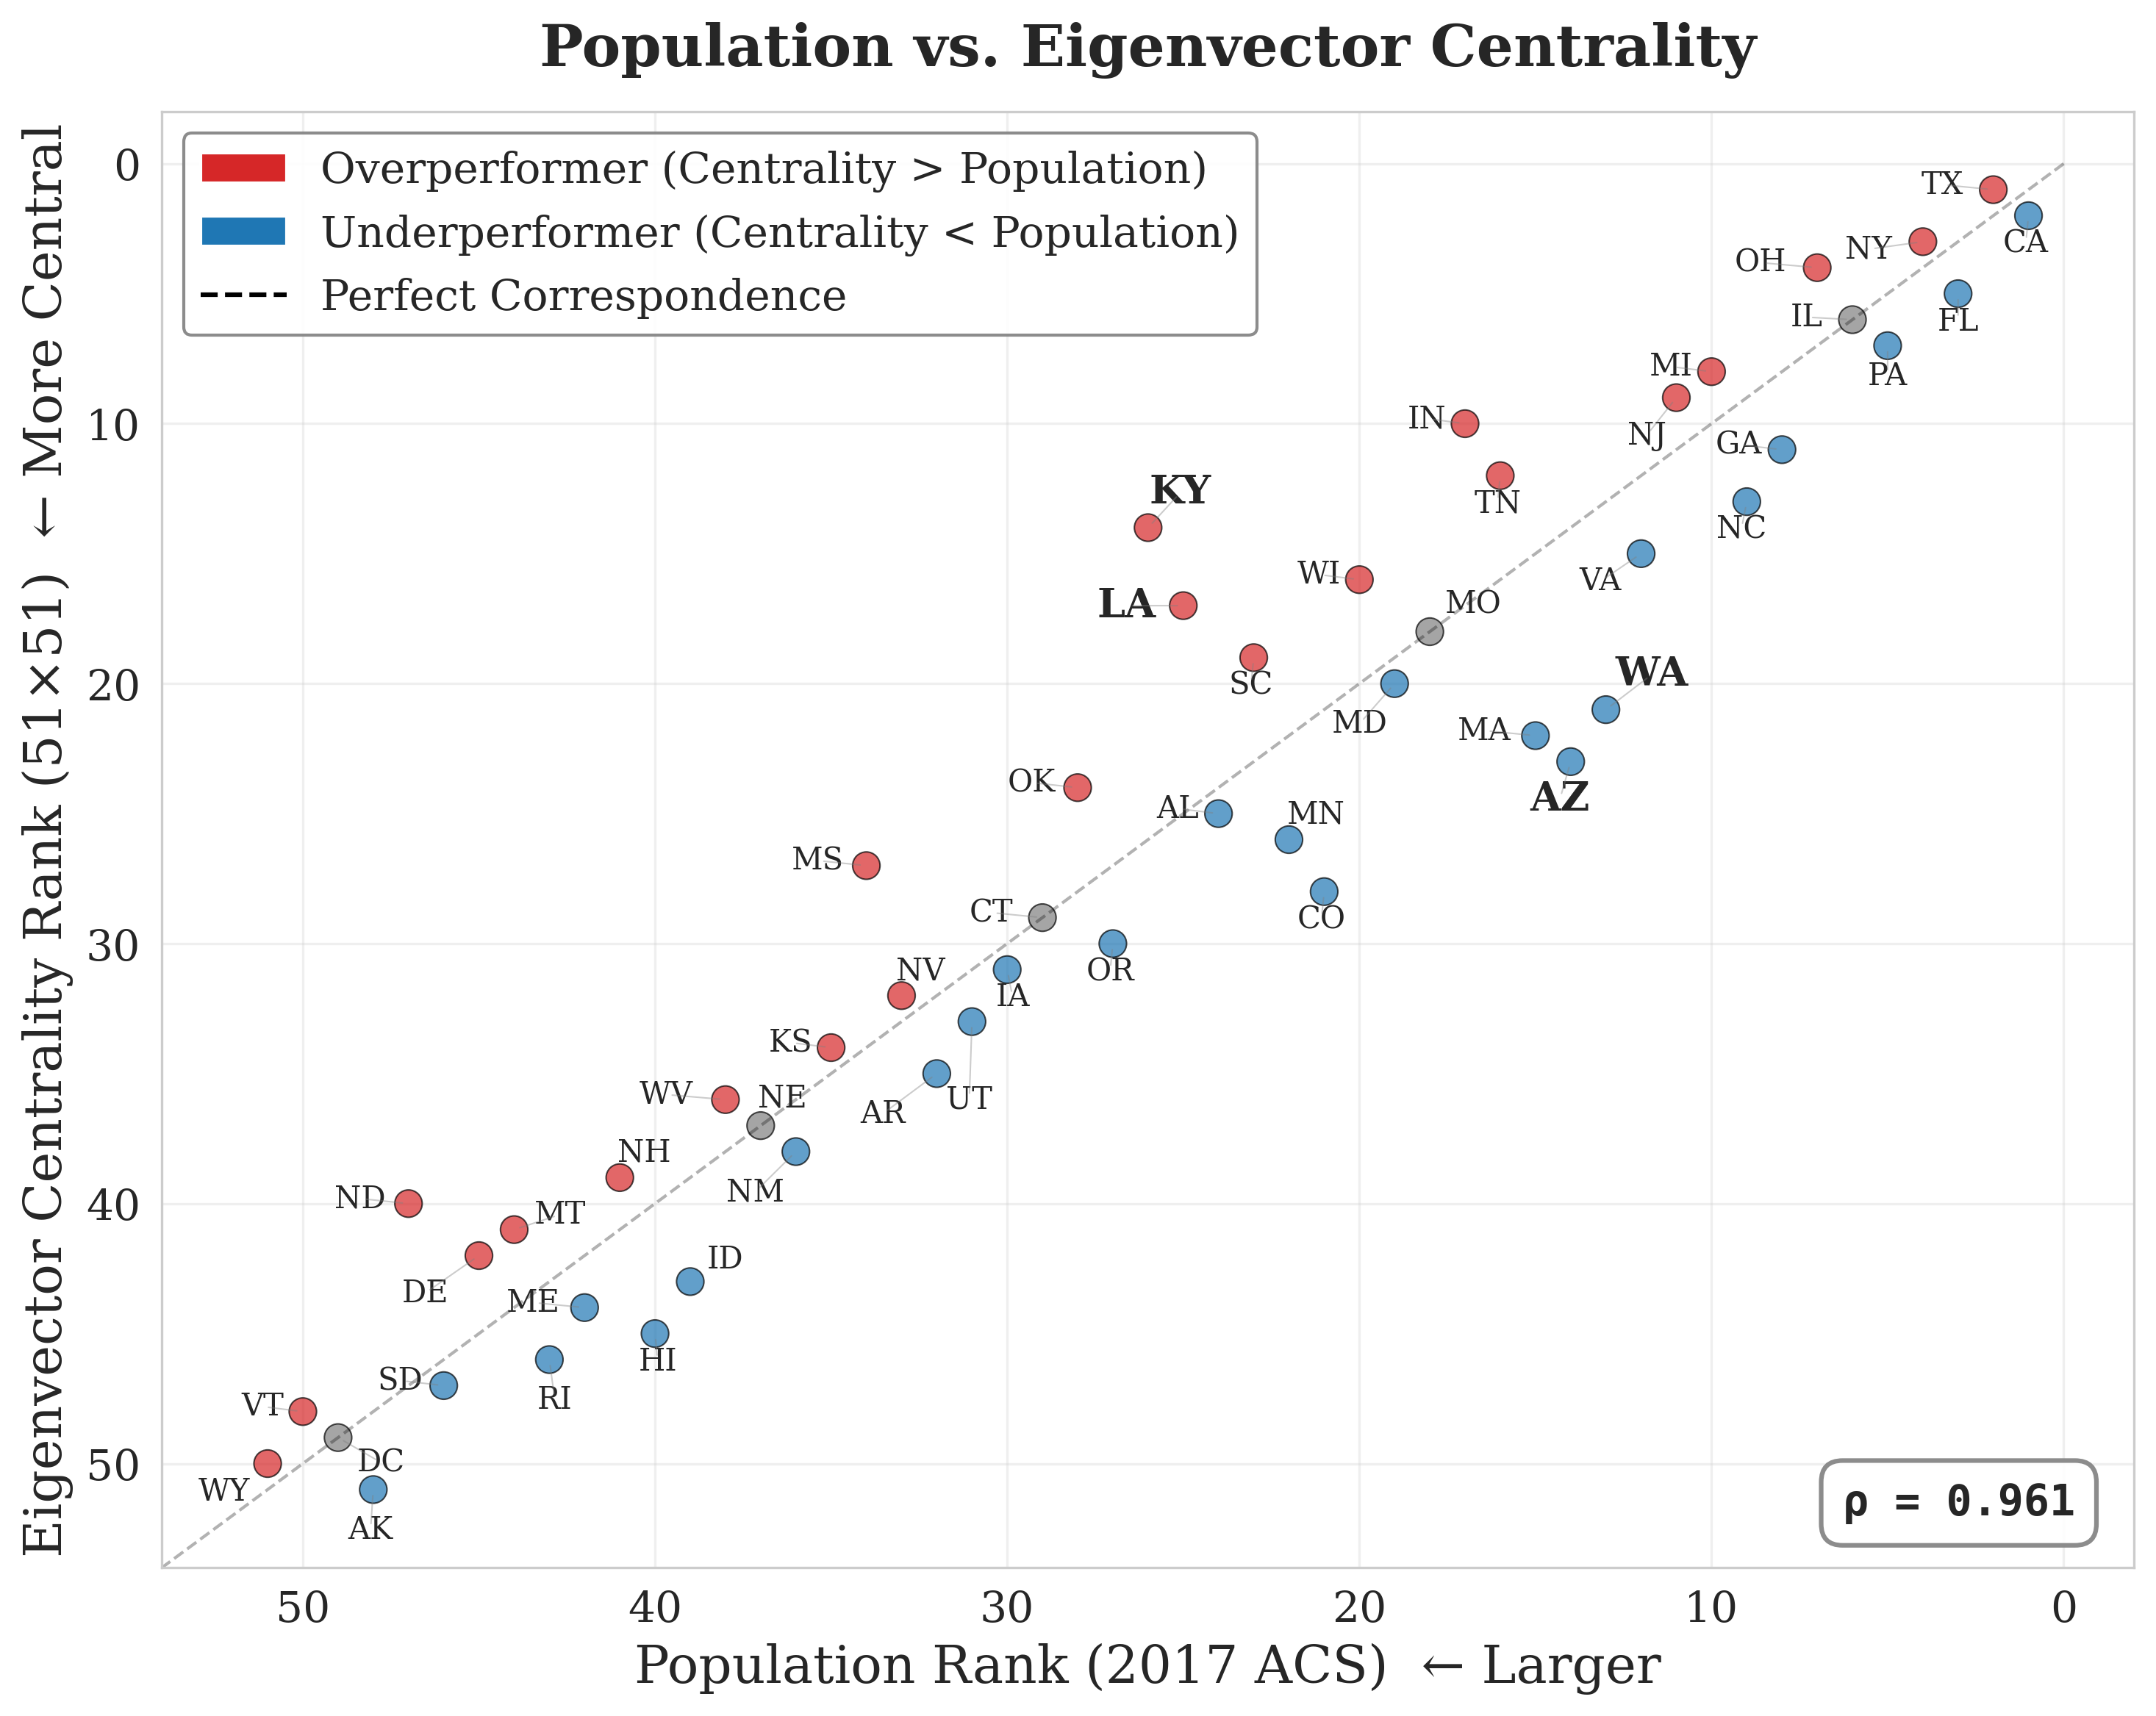
\includegraphics[width=\textwidth]{figures/pop_vs_eigenvector_scatter.png}
\caption[Population rank vs.\ eigenvector centrality rank ($\rho = 0.961$).]{Population rank vs.\ eigenvector centrality rank ($\rho = 0.961$). Population shows an even stronger correlation with eigenvector centrality than GDP, consistent with the GDP--population correlation ($r = 0.98$).}
\label{fig:pop_eigenvector_scatter}
\end{figure}

\begin{figure}[ht]
\centering
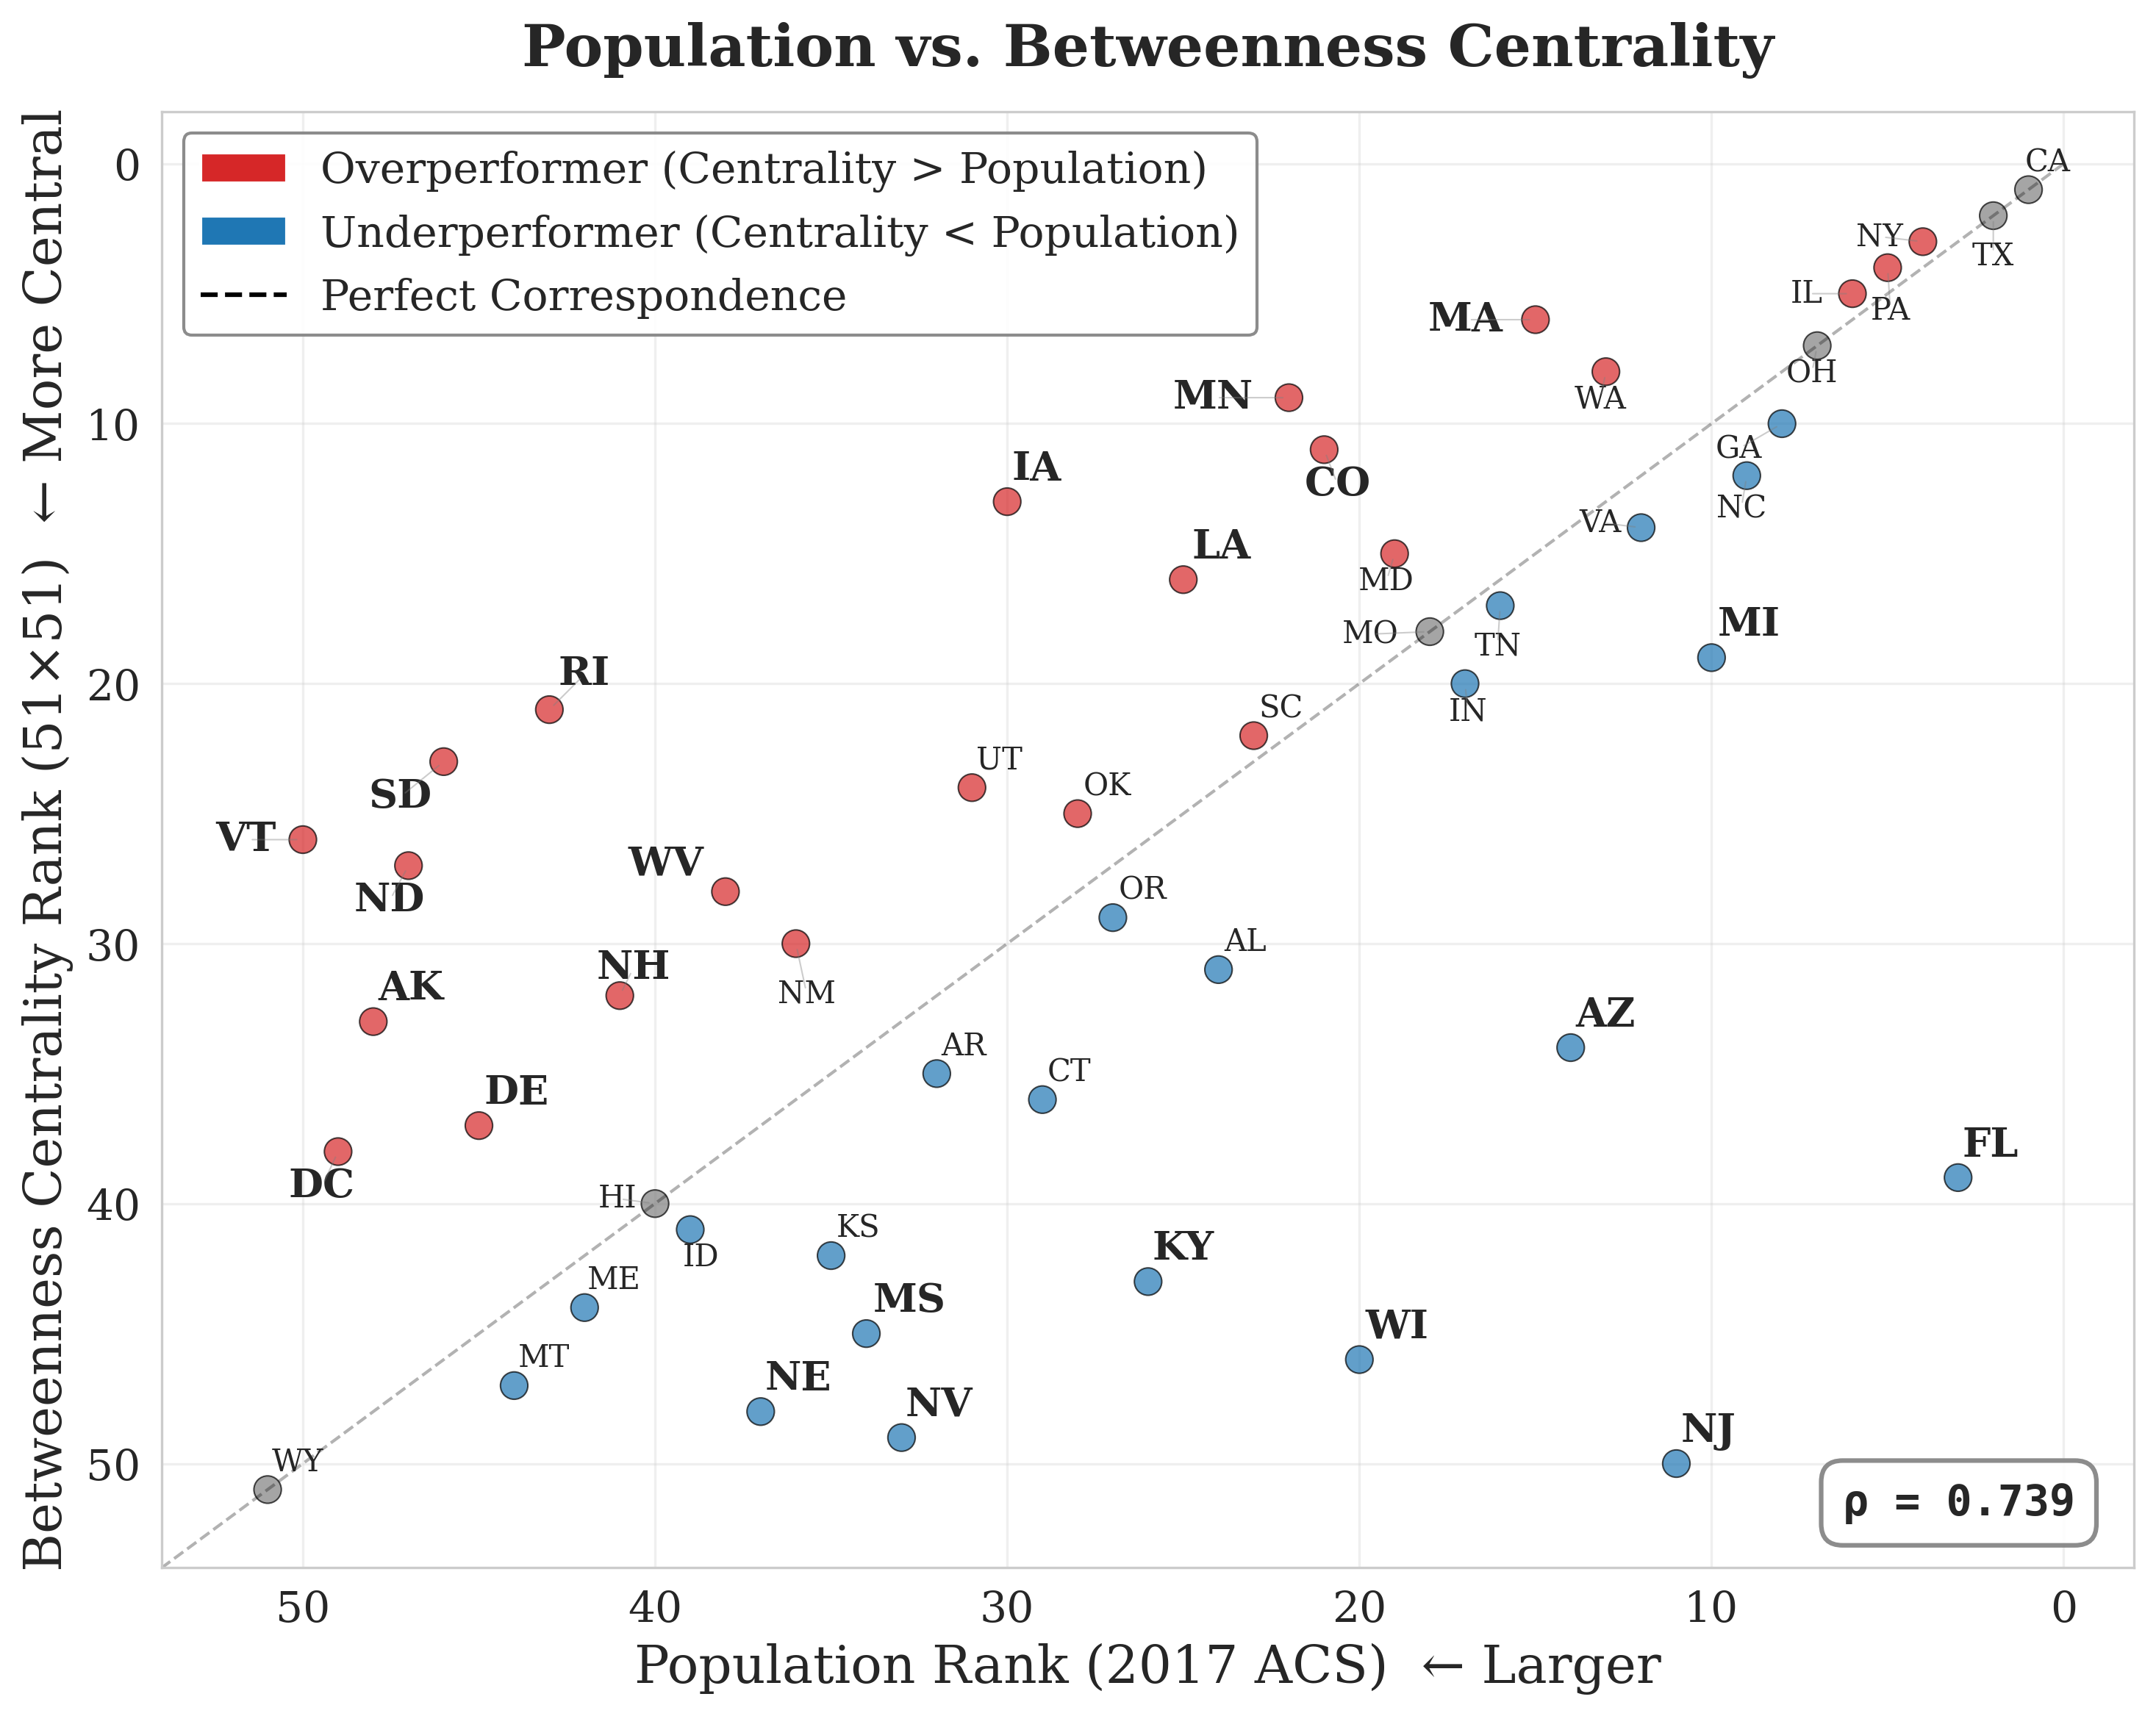
\includegraphics[width=\textwidth]{figures/pop_vs_betweenness_scatter.png}
\caption[Population rank vs.\ betweenness centrality rank ($\rho = 0.739$).]{Population rank vs.\ betweenness centrality rank ($\rho = 0.739$). Betweenness correlates only moderately with population, confirming that bridging position reflects network topology rather than size.}
\label{fig:pop_betweenness_scatter}
\end{figure}

\begin{figure}[ht]
\centering
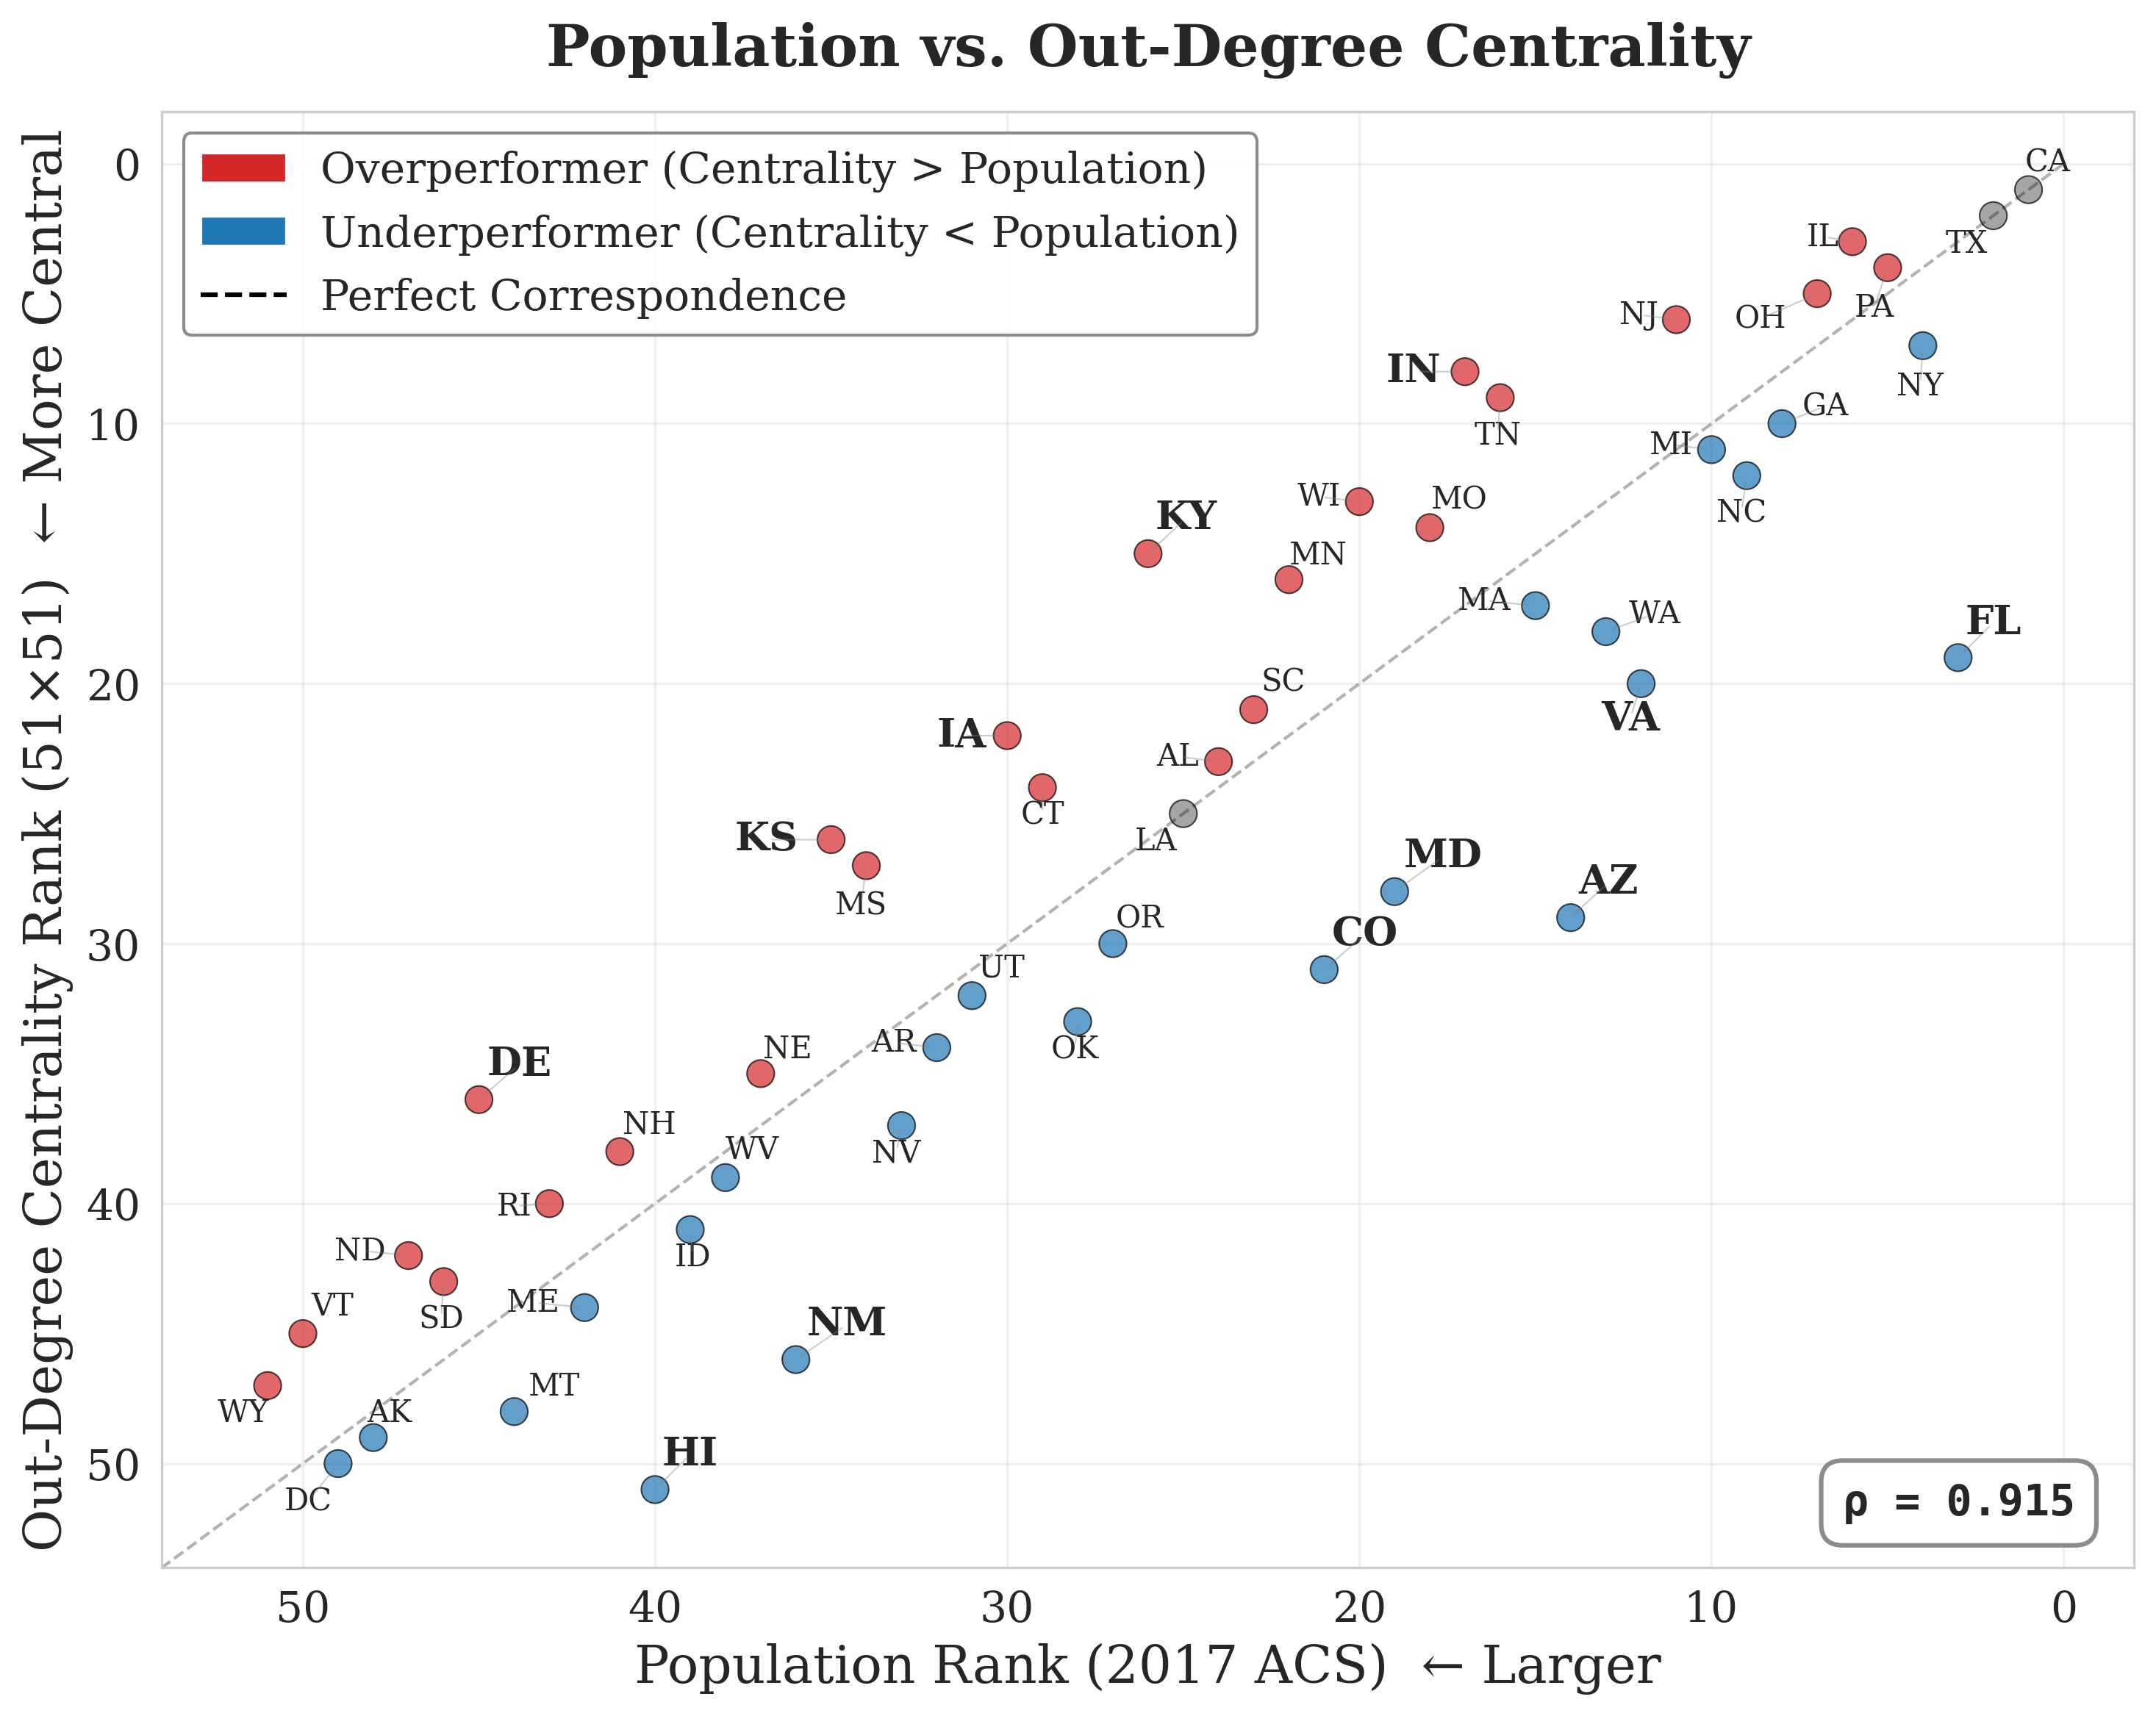
\includegraphics[width=\textwidth]{figures/pop_vs_out_degree_scatter.png}
\caption[Population rank vs.\ weighted out-degree centrality rank ($\rho = 0.915$).]{Population rank vs.\ weighted out-degree centrality rank ($\rho = 0.915$). Distribution capacity tracks population similarly to GDP.}
\label{fig:pop_outdegree_scatter}
\end{figure}

\begin{figure}[ht]
\centering
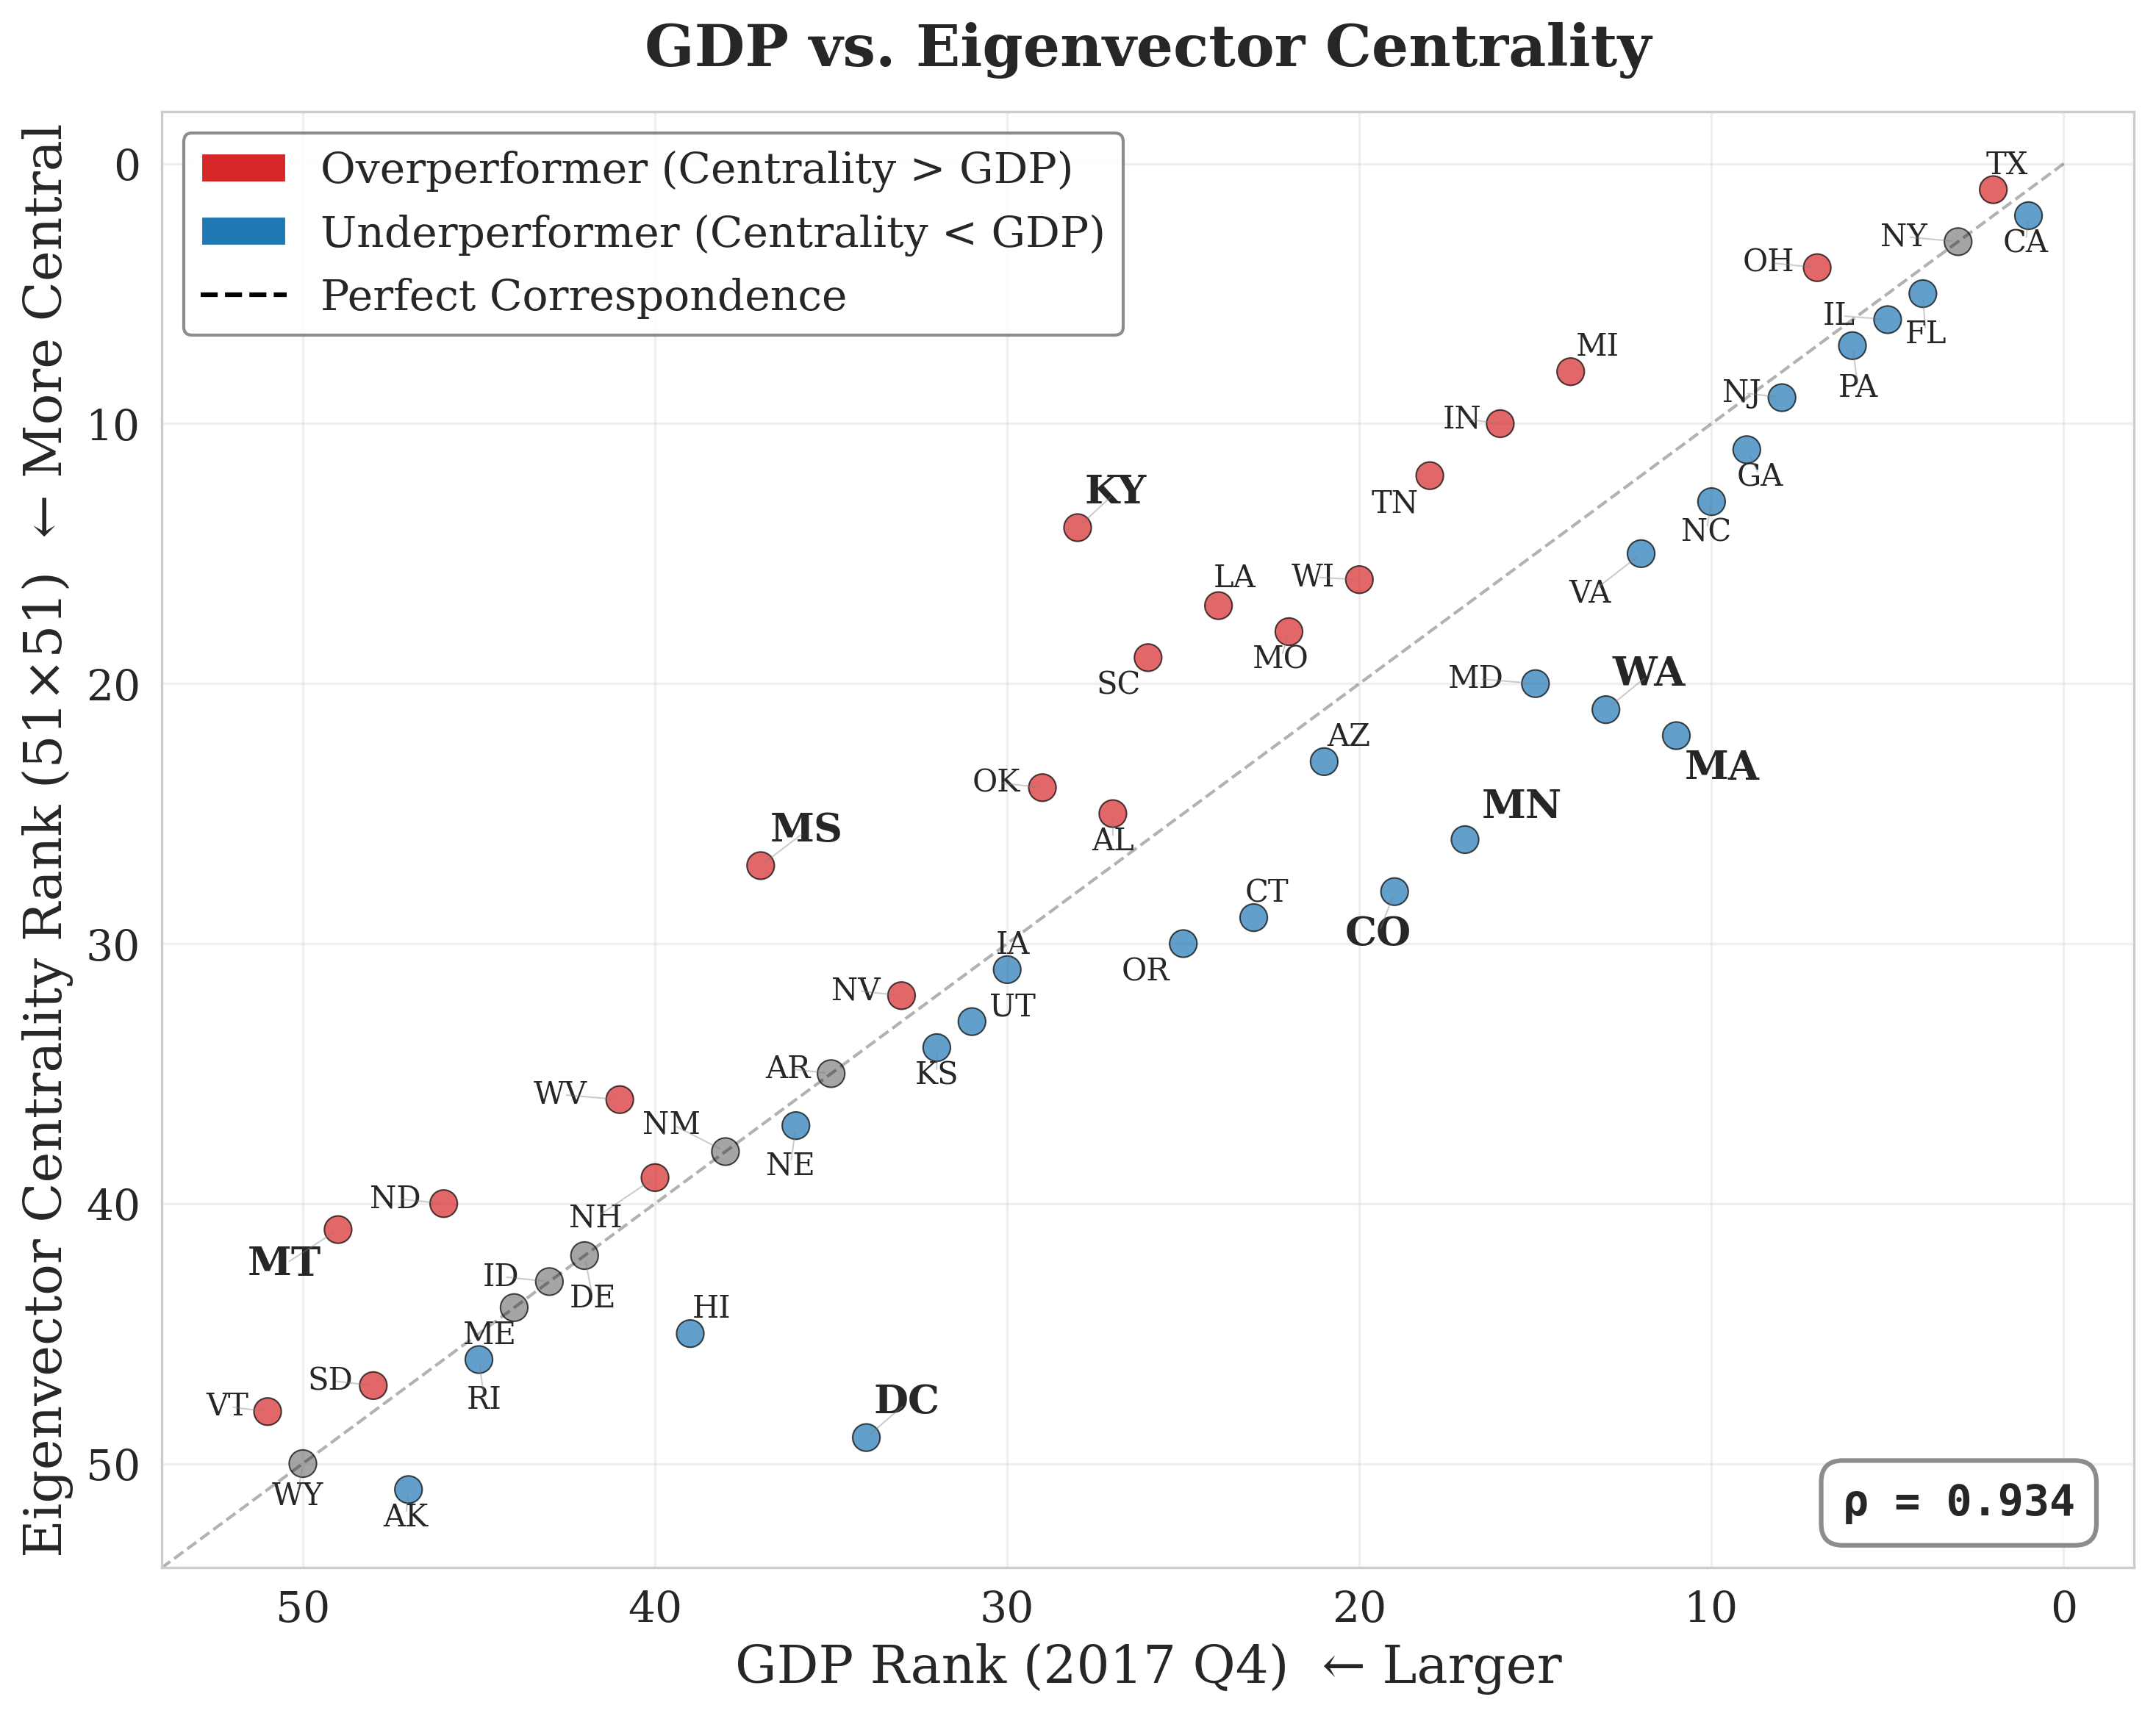
\includegraphics[width=\textwidth]{figures/gdp_vs_eigenvector_scatter.png}
\caption[GDP rank vs.\ eigenvector centrality rank ($\rho = 0.934$).]{GDP rank vs.\ eigenvector centrality rank ($\rho =
0.934$). This figure also appears in the main text
(Figure~\ref{fig:gdp_scatter}); it is reproduced here for
completeness alongside the other five centrality--control
combinations.}
\label{fig:gdp_eigenvector_scatter_appendix}
\end{figure}

\begin{figure}[ht]
\centering                                                         
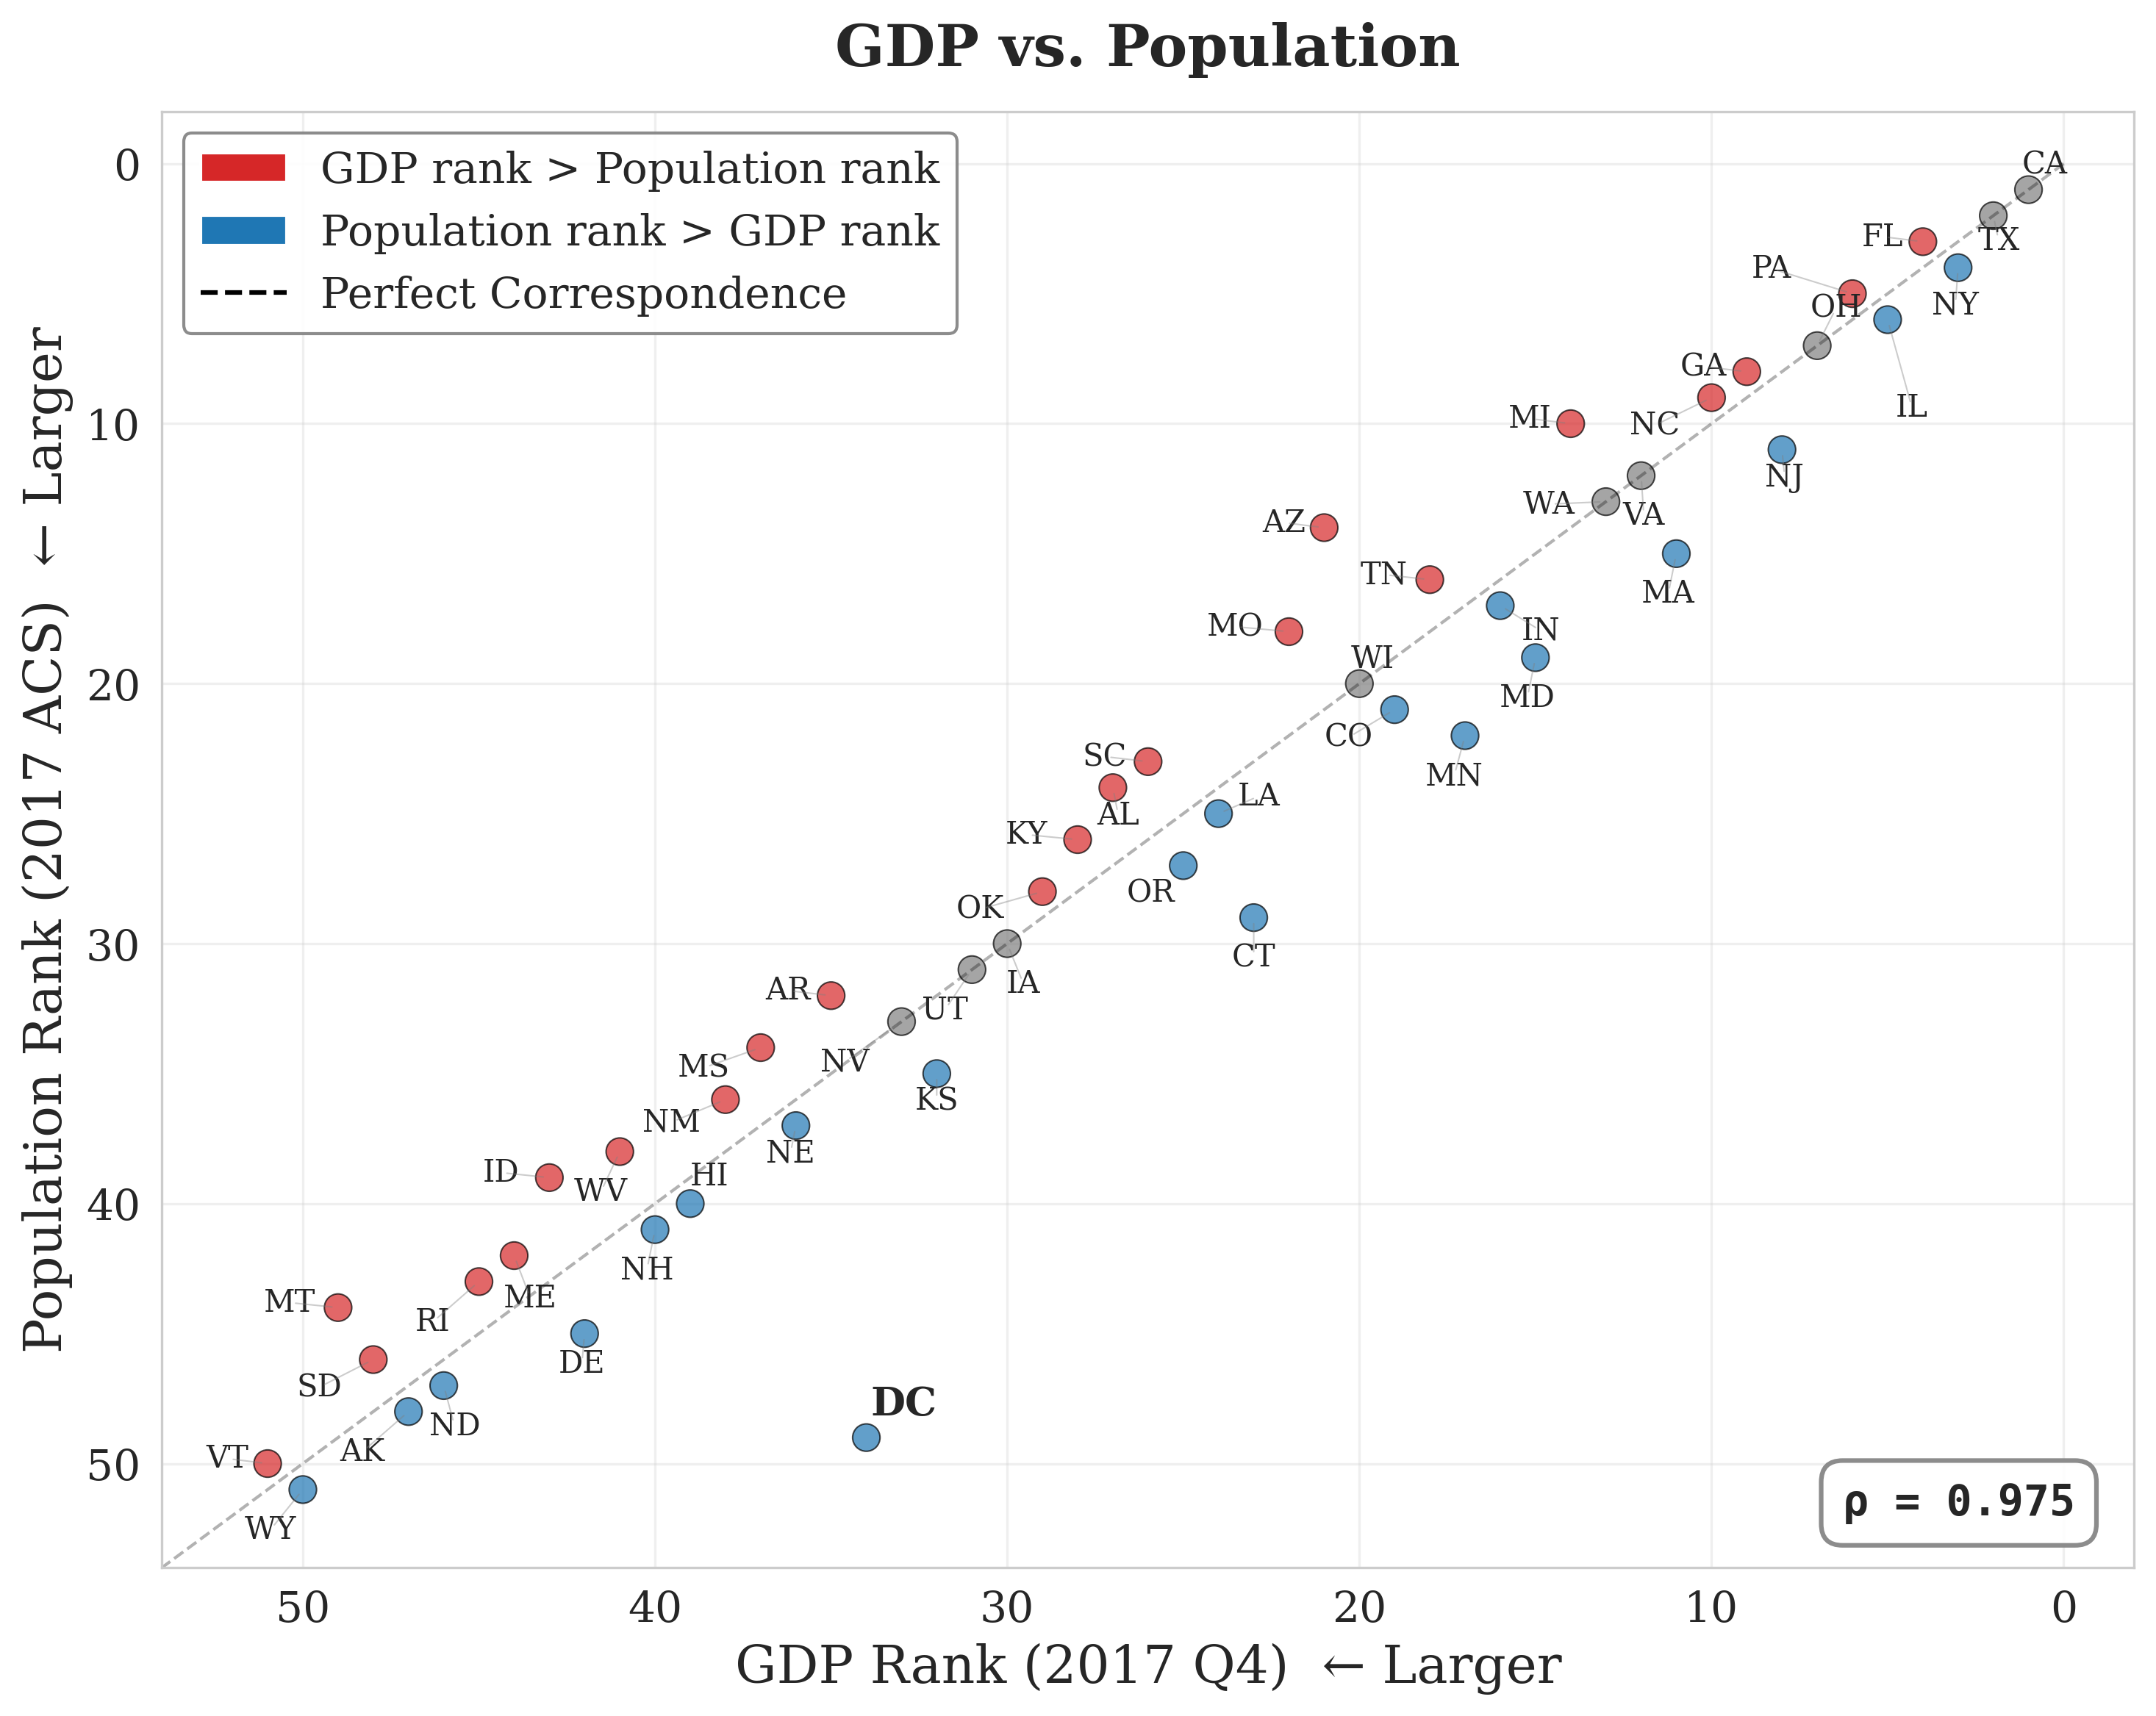
\includegraphics[width=\textwidth]{figures/gdp_vs_population_scatter.png}
\caption[GDP rank vs.\ population rank (Spearman $\rho = 0.975$).]{GDP rank vs.\ population rank (Spearman $\rho = 0.975$). The near-perfect correlation confirms that GDP and population produce consistent control rankings, validating the use of either as a baseline for centrality divergence analysis.}                 
\label{fig:gdp_population_scatter}     
\end{figure}

\begin{table}[ht]
\centering
\caption[Spearman rank correlations ($\rho$) between control variables and centrality measures.]{Spearman rank correlations ($\rho$) between control variables and centrality measures (51$\times$51 domestic network). All correlations significant at $p < 0.001$.}
\label{tab:rho_correlations}
\begin{tabular}{l c c c}
\hline
& \textbf{Eigenvector} & \textbf{Betweenness} & \textbf{Out-Degree} \\
\hline
\textbf{GDP} & $0.934$ & $0.763$ & $0.904$ \\
\textbf{Population} & $0.961$ & $0.739$ & $0.915$ \\
\hline
\end{tabular}
\end{table}

\FloatBarrier

\chapter{Node Distribution}
\label{appendix:node_distribution}

Table~\ref{tab:trade_balance} reports trade flow metrics for all 51 domestic nodes, sorted by total outbound trade.

\begin{footnotesize}
\begin{singlespace}
\begin{longtable}{l r r r r r r r}
\caption[Trade Flow Metrics by State (51$\times$51 Domestic Network, 2017 CFS).]{Trade Flow Metrics by State (51$\times$51 Domestic Network, 2017 CFS). Net In and Net Out are total inbound and outbound commodity flows in billions USD. Ratio = Net In / Net Out (values $>$1 indicate net importer). RoW In Share and RoW Out Share are each state\textquotesingle s fraction of total cross-border flows with the Rest of World node (52$\times$52 network). GDP in billions (2017 Q4 BEA). Pop in millions (2017 ACS). States sorted by total outbound trade.}
\label{tab:trade_balance} \\
\hline
\textbf{State} & \textbf{Net In (\$B)} & \textbf{Net Out (\$B)} & \textbf{Ratio} & \textbf{RoW In} & \textbf{RoW Out} & \textbf{GDP (\$B)} & \textbf{Pop (M)} \\
\hline
\endfirsthead
\hline
\textbf{State} & \textbf{Net In (\$B)} & \textbf{Net Out (\$B)} & \textbf{Ratio} & \textbf{RoW In} & \textbf{RoW Out} & \textbf{GDP (\$B)} & \textbf{Pop (M)} \\
\hline
\endhead
\hline
\endfoot
CA & 480.7 & 610.1 & 0.788 & 19.1\% & 11.7\% & 2802.3 & 39.54 \\
TX & 569.8 & 458.8 & 1.242 & 11.5\% & 17.6\% & 1747.2 & 28.30 \\
IL & 375.6 & 458.1 & 0.820 & 5.7\% & 4.3\% & 835.6 & 12.80 \\
PA & 329.4 & 414.5 & 0.795 & 3.6\% & 2.6\% & 767.6 & 12.81 \\
OH & 349.0 & 361.3 & 0.966 & 3.0\% & 3.3\% & 661.1 & 11.66 \\
NJ & 262.1 & 318.7 & 0.823 & 4.9\% & 2.3\% & 601.9 & 9.01 \\
NY & 417.9 & 309.2 & 1.352 & 5.2\% & 5.2\% & 1564.3 & 19.85 \\
IN & 252.2 & 295.5 & 0.853 & 2.6\% & 2.6\% & 364.6 & 6.67 \\
TN & 245.7 & 293.5 & 0.837 & 3.4\% & 2.2\% & 352.0 & 6.72 \\
GA & 289.8 & 286.8 & 1.010 & 4.0\% & 2.5\% & 563.8 & 10.43 \\
MI & 276.0 & 278.1 & 0.993 & 6.1\% & 4.0\% & 512.8 & 9.96 \\
NC & 212.2 & 266.6 & 0.796 & 2.1\% & 2.2\% & 547.2 & 10.27 \\
WI & 175.0 & 207.9 & 0.842 & 1.2\% & 1.5\% & 330.8 & 5.80 \\
MO & 159.4 & 189.0 & 0.844 & 0.8\% & 1.0\% & 309.2 & 6.11 \\
KY & 172.3 & 177.5 & 0.971 & 2.1\% & 2.1\% & 205.9 & 4.45 \\
MN & 132.8 & 172.5 & 0.770 & 1.3\% & 1.4\% & 353.3 & 5.58 \\
MA & 158.4 & 168.8 & 0.938 & 1.5\% & 1.9\% & 537.1 & 6.86 \\
WA & 161.0 & 162.0 & 0.994 & 2.1\% & 5.6\% & 517.2 & 7.41 \\
FL & 354.0 & 156.8 & 2.257 & 3.2\% & 3.7\% & 984.1 & 20.98 \\
VA & 184.8 & 144.7 & 1.276 & 1.3\% & 1.2\% & 517.5 & 8.47 \\
SC & 149.2 & 141.5 & 1.054 & 1.6\% & 2.1\% & 222.2 & 5.02 \\
IA & 102.5 & 140.7 & 0.728 & 0.4\% & 0.9\% & 191.1 & 3.15 \\
AL & 123.0 & 140.3 & 0.877 & 1.0\% & 1.4\% & 213.9 & 4.87 \\
CT & 93.5 & 126.4 & 0.740 & 0.7\% & 0.9\% & 265.9 & 3.59 \\
LA & 124.7 & 117.2 & 1.064 & 1.6\% & 3.7\% & 251.1 & 4.68 \\
KS & 87.4 & 112.8 & 0.775 & 0.5\% & 0.7\% & 160.4 & 2.91 \\
MS & 103.4 & 106.1 & 0.975 & 0.8\% & 0.7\% & 113.4 & 2.98 \\
MD & 148.8 & 100.6 & 1.479 & 1.4\% & 0.6\% & 400.6 & 6.05 \\
AZ & 113.0 & 93.9 & 1.203 & 0.8\% & 1.4\% & 327.9 & 7.02 \\
OR & 97.9 & 88.4 & 1.108 & 0.8\% & 1.4\% & 240.7 & 4.14 \\
CO & 96.1 & 82.8 & 1.161 & 0.5\% & 0.6\% & 351.7 & 5.61 \\
UT & 78.0 & 80.8 & 0.966 & 0.6\% & 0.8\% & 169.1 & 3.10 \\
OK & 102.7 & 74.1 & 1.387 & 0.5\% & 0.4\% & 192.3 & 3.93 \\
AR & 73.5 & 71.4 & 1.030 & 0.4\% & 0.4\% & 126.3 & 3.00 \\
NE & 55.2 & 63.7 & 0.867 & 0.2\% & 0.5\% & 123.1 & 1.92 \\
DE & 28.0 & 39.7 & 0.706 & 0.3\% & 0.3\% & 75.0 & 0.96 \\
NV & 70.4 & 39.3 & 1.788 & 0.5\% & 0.8\% & 160.1 & 3.00 \\
NH & 50.4 & 38.6 & 1.303 & 0.5\% & 0.3\% & 82.0 & 1.34 \\
WV & 48.0 & 38.2 & 1.257 & 0.1\% & 0.5\% & 78.8 & 1.82 \\
RI & 21.3 & 36.7 & 0.579 & 0.4\% & 0.2\% & 60.7 & 1.06 \\
ID & 35.0 & 28.4 & 1.235 & 0.2\% & 0.3\% & 73.3 & 1.72 \\
ND & 39.7 & 25.8 & 1.539 & 0.1\% & 0.4\% & 55.9 & 0.76 \\
SD & 25.3 & 22.8 & 1.111 & 0.0\% & 0.1\% & 50.3 & 0.87 \\
ME & 31.6 & 20.8 & 1.524 & 0.1\% & 0.2\% & 62.5 & 1.34 \\
VT & 18.3 & 18.4 & 0.993 & 0.1\% & 0.2\% & 32.6 & 0.62 \\
NM & 36.4 & 14.5 & 2.501 & 0.1\% & 0.2\% & 99.1 & 2.09 \\
WY & 17.6 & 11.6 & 1.511 & 0.1\% & 0.1\% & 41.4 & 0.58 \\
MT & 39.0 & 10.4 & 3.741 & 0.2\% & 0.1\% & 48.6 & 1.05 \\
AK & 17.4 & 3.6 & 4.889 & 0.1\% & 0.4\% & 54.4 & 0.74 \\
DC & 18.9 & 1.1 & 17.224 & 0.0\% & 0.1\% & 134.0 & 0.69 \\
HI & 17.6 & 0.9 & 18.814 & 0.3\% & 0.2\% & 89.3 & 1.43 \\
\end{longtable}
\end{singlespace}
\end{footnotesize}

Table~\ref{tab:node_distribution} provides the complete centrality data for all 51 domestic nodes, sorted by eigenvector centrality rank. This table enables readers to look up any state's structural position across all three centrality measures alongside its economic size (GDP) and population.

\begin{footnotesize}
\begin{singlespace}
\begin{longtable}{l r r r r r r r r}
\caption[Complete centrality data for all 51 domestic nodes sorted by eigenvector centrality rank.]{Pop.\ in millions (2017 ACS). GDP in billions (2017 Q4 BEA). Betw.\ = betweenness centrality (normalized). Eig.\ = eigenvector centrality (normalized). Out-D.\ = weighted out-degree centrality (normalized). Rk = rank (1 = highest). States sorted by eigenvector centrality rank.} \label{tab:node_distribution} \\

\hline
\textbf{State} & \textbf{Pop (M)} & \textbf{GDP (\$B)} & \textbf{Betw.} & \textbf{Rk} & \textbf{Eig.} & \textbf{Rk} & \textbf{Out-D.} & \textbf{Rk} \\
\hline
\endfirsthead
\hline
\textbf{State} & \textbf{Pop (M)} & \textbf{GDP (\$B)} & \textbf{Betw.} & \textbf{Rk} & \textbf{Eig.} & \textbf{Rk} & \textbf{Out-D.} & \textbf{Rk} \\
\hline
\endhead
\hline
\endfoot
TX & 28.30 & 1747.2 & 0.2629 & 2 & 0.3714 & 1 & 0.7520 & 2 \\
CA & 39.54 & 2802.3 & 0.5061 & 1 & 0.3091 & 2 & 1.0000 & 1 \\
NY & 19.85 & 1564.3 & 0.2033 & 3 & 0.2902 & 3 & 0.5068 & 7 \\
OH & 11.66 & 661.1 & 0.1008 & 7 & 0.2676 & 4 & 0.5922 & 5 \\
FL & 20.98 & 984.1 & 0.0000 & 21 & 0.2637 & 5 & 0.2570 & 19 \\
IL & 12.80 & 835.6 & 0.1449 & 5 & 0.2523 & 6 & 0.7508 & 3 \\
PA & 12.81 & 767.6 & 0.1678 & 4 & 0.2413 & 7 & 0.6794 & 4 \\
MI & 9.96 & 512.8 & 0.0041 & 19 & 0.2167 & 8 & 0.4559 & 11 \\
NJ & 9.01 & 601.9 & 0.0000 & 21 & 0.2119 & 9 & 0.5223 & 6 \\
IN & 6.67 & 364.6 & 0.0029 & 20 & 0.2007 & 10 & 0.4843 & 8 \\
GA & 10.43 & 563.8 & 0.0473 & 10 & 0.1977 & 11 & 0.4700 & 10 \\
TN & 6.72 & 352.0 & 0.0106 & 17 & 0.1648 & 12 & 0.4811 & 9 \\
NC & 10.27 & 547.2 & 0.0351 & 12 & 0.1502 & 13 & 0.4369 & 12 \\
KY & 4.45 & 205.9 & 0.0000 & 21 & 0.1355 & 14 & 0.2909 & 15 \\
VA & 8.47 & 517.5 & 0.0249 & 14 & 0.1281 & 15 & 0.2372 & 20 \\
WI & 5.80 & 330.8 & 0.0000 & 21 & 0.1278 & 16 & 0.3407 & 13 \\
LA & 4.68 & 251.1 & 0.0155 & 16 & 0.1114 & 17 & 0.1922 & 25 \\
MO & 6.11 & 309.2 & 0.0057 & 18 & 0.1111 & 18 & 0.3097 & 14 \\
SC & 5.02 & 222.2 & 0.0000 & 21 & 0.1106 & 19 & 0.2319 & 21 \\
MD & 6.05 & 400.6 & 0.0200 & 15 & 0.1046 & 20 & 0.1649 & 28 \\
WA & 7.41 & 517.2 & 0.0980 & 8 & 0.1025 & 21 & 0.2655 & 18 \\
MA & 6.86 & 537.1 & 0.1131 & 6 & 0.0974 & 22 & 0.2766 & 17 \\
AZ & 7.02 & 327.9 & 0.0000 & 21 & 0.0972 & 23 & 0.1539 & 29 \\
OK & 3.93 & 192.3 & 0.0000 & 21 & 0.0937 & 24 & 0.1214 & 33 \\
AL & 4.87 & 213.9 & 0.0000 & 21 & 0.0920 & 25 & 0.2299 & 23 \\
MN & 5.58 & 353.3 & 0.0600 & 9 & 0.0843 & 26 & 0.2827 & 16 \\
MS & 2.98 & 113.4 & 0.0000 & 21 & 0.0762 & 27 & 0.1739 & 27 \\
CO & 5.61 & 351.7 & 0.0400 & 11 & 0.0697 & 28 & 0.1357 & 31 \\
CT & 3.59 & 265.9 & 0.0000 & 21 & 0.0666 & 29 & 0.2072 & 24 \\
OR & 4.14 & 240.7 & 0.0000 & 21 & 0.0664 & 30 & 0.1448 & 30 \\
IA & 3.15 & 191.1 & 0.0257 & 13 & 0.0647 & 31 & 0.2306 & 22 \\
NV & 3.00 & 160.1 & 0.0000 & 21 & 0.0635 & 32 & 0.0645 & 37 \\
UT & 3.10 & 169.1 & 0.0000 & 21 & 0.0608 & 33 & 0.1324 & 32 \\
KS & 2.91 & 160.4 & 0.0000 & 21 & 0.0593 & 34 & 0.1849 & 26 \\
AR & 3.00 & 126.3 & 0.0000 & 21 & 0.0547 & 35 & 0.1170 & 34 \\
WV & 1.82 & 78.8 & 0.0000 & 21 & 0.0378 & 36 & 0.0625 & 39 \\
NE & 1.92 & 123.1 & 0.0000 & 21 & 0.0319 & 37 & 0.1044 & 35 \\
NM & 2.09 & 99.1 & 0.0000 & 21 & 0.0316 & 38 & 0.0238 & 46 \\
NH & 1.34 & 82.0 & 0.0000 & 21 & 0.0273 & 39 & 0.0633 & 38 \\
ND & 0.76 & 55.9 & 0.0000 & 21 & 0.0258 & 40 & 0.0423 & 42 \\
MT & 1.05 & 48.6 & 0.0000 & 21 & 0.0237 & 41 & 0.0171 & 48 \\
DE & 0.96 & 75.0 & 0.0000 & 21 & 0.0199 & 42 & 0.0651 & 36 \\
ID & 1.72 & 73.3 & 0.0000 & 21 & 0.0190 & 43 & 0.0465 & 41 \\
ME & 1.34 & 62.5 & 0.0000 & 21 & 0.0190 & 44 & 0.0340 & 44 \\
HI & 1.43 & 89.3 & 0.0000 & 21 & 0.0168 & 45 & 0.0015 & 51 \\
RI & 1.06 & 60.7 & 0.0000 & 21 & 0.0120 & 46 & 0.0602 & 40 \\
SD & 0.87 & 50.3 & 0.0000 & 21 & 0.0119 & 47 & 0.0373 & 43 \\
VT & 0.62 & 32.6 & 0.0000 & 21 & 0.0119 & 48 & 0.0302 & 45 \\
DC & 0.69 & 134.0 & 0.0000 & 21 & 0.0112 & 49 & 0.0018 & 50 \\
WY & 0.58 & 41.4 & 0.0000 & 21 & 0.0094 & 50 & 0.0191 & 47 \\
AK & 0.74 & 54.4 & 0.0000 & 21 & 0.0093 & 51 & 0.0058 & 49 \\
\end{longtable}
\end{singlespace}
\end{footnotesize}


\chapter{Boundary Sensitivity Rank Scatter Plots}
\label{appendix:rank_scatters}

Figures~\ref{fig:rank_eigenvector}--\ref{fig:rank_outdegree} present rank stability scatter plots for eigenvector
and out-degree centrality under boundary specification change (51$\times$51 vs 52$\times$52). The betweenness
scatter plot, which shows the most dramatic sensitivity, is presented in the main text
(Figure~\ref{fig:rank_betweenness}).

\begin{figure}[htbp]
\centering
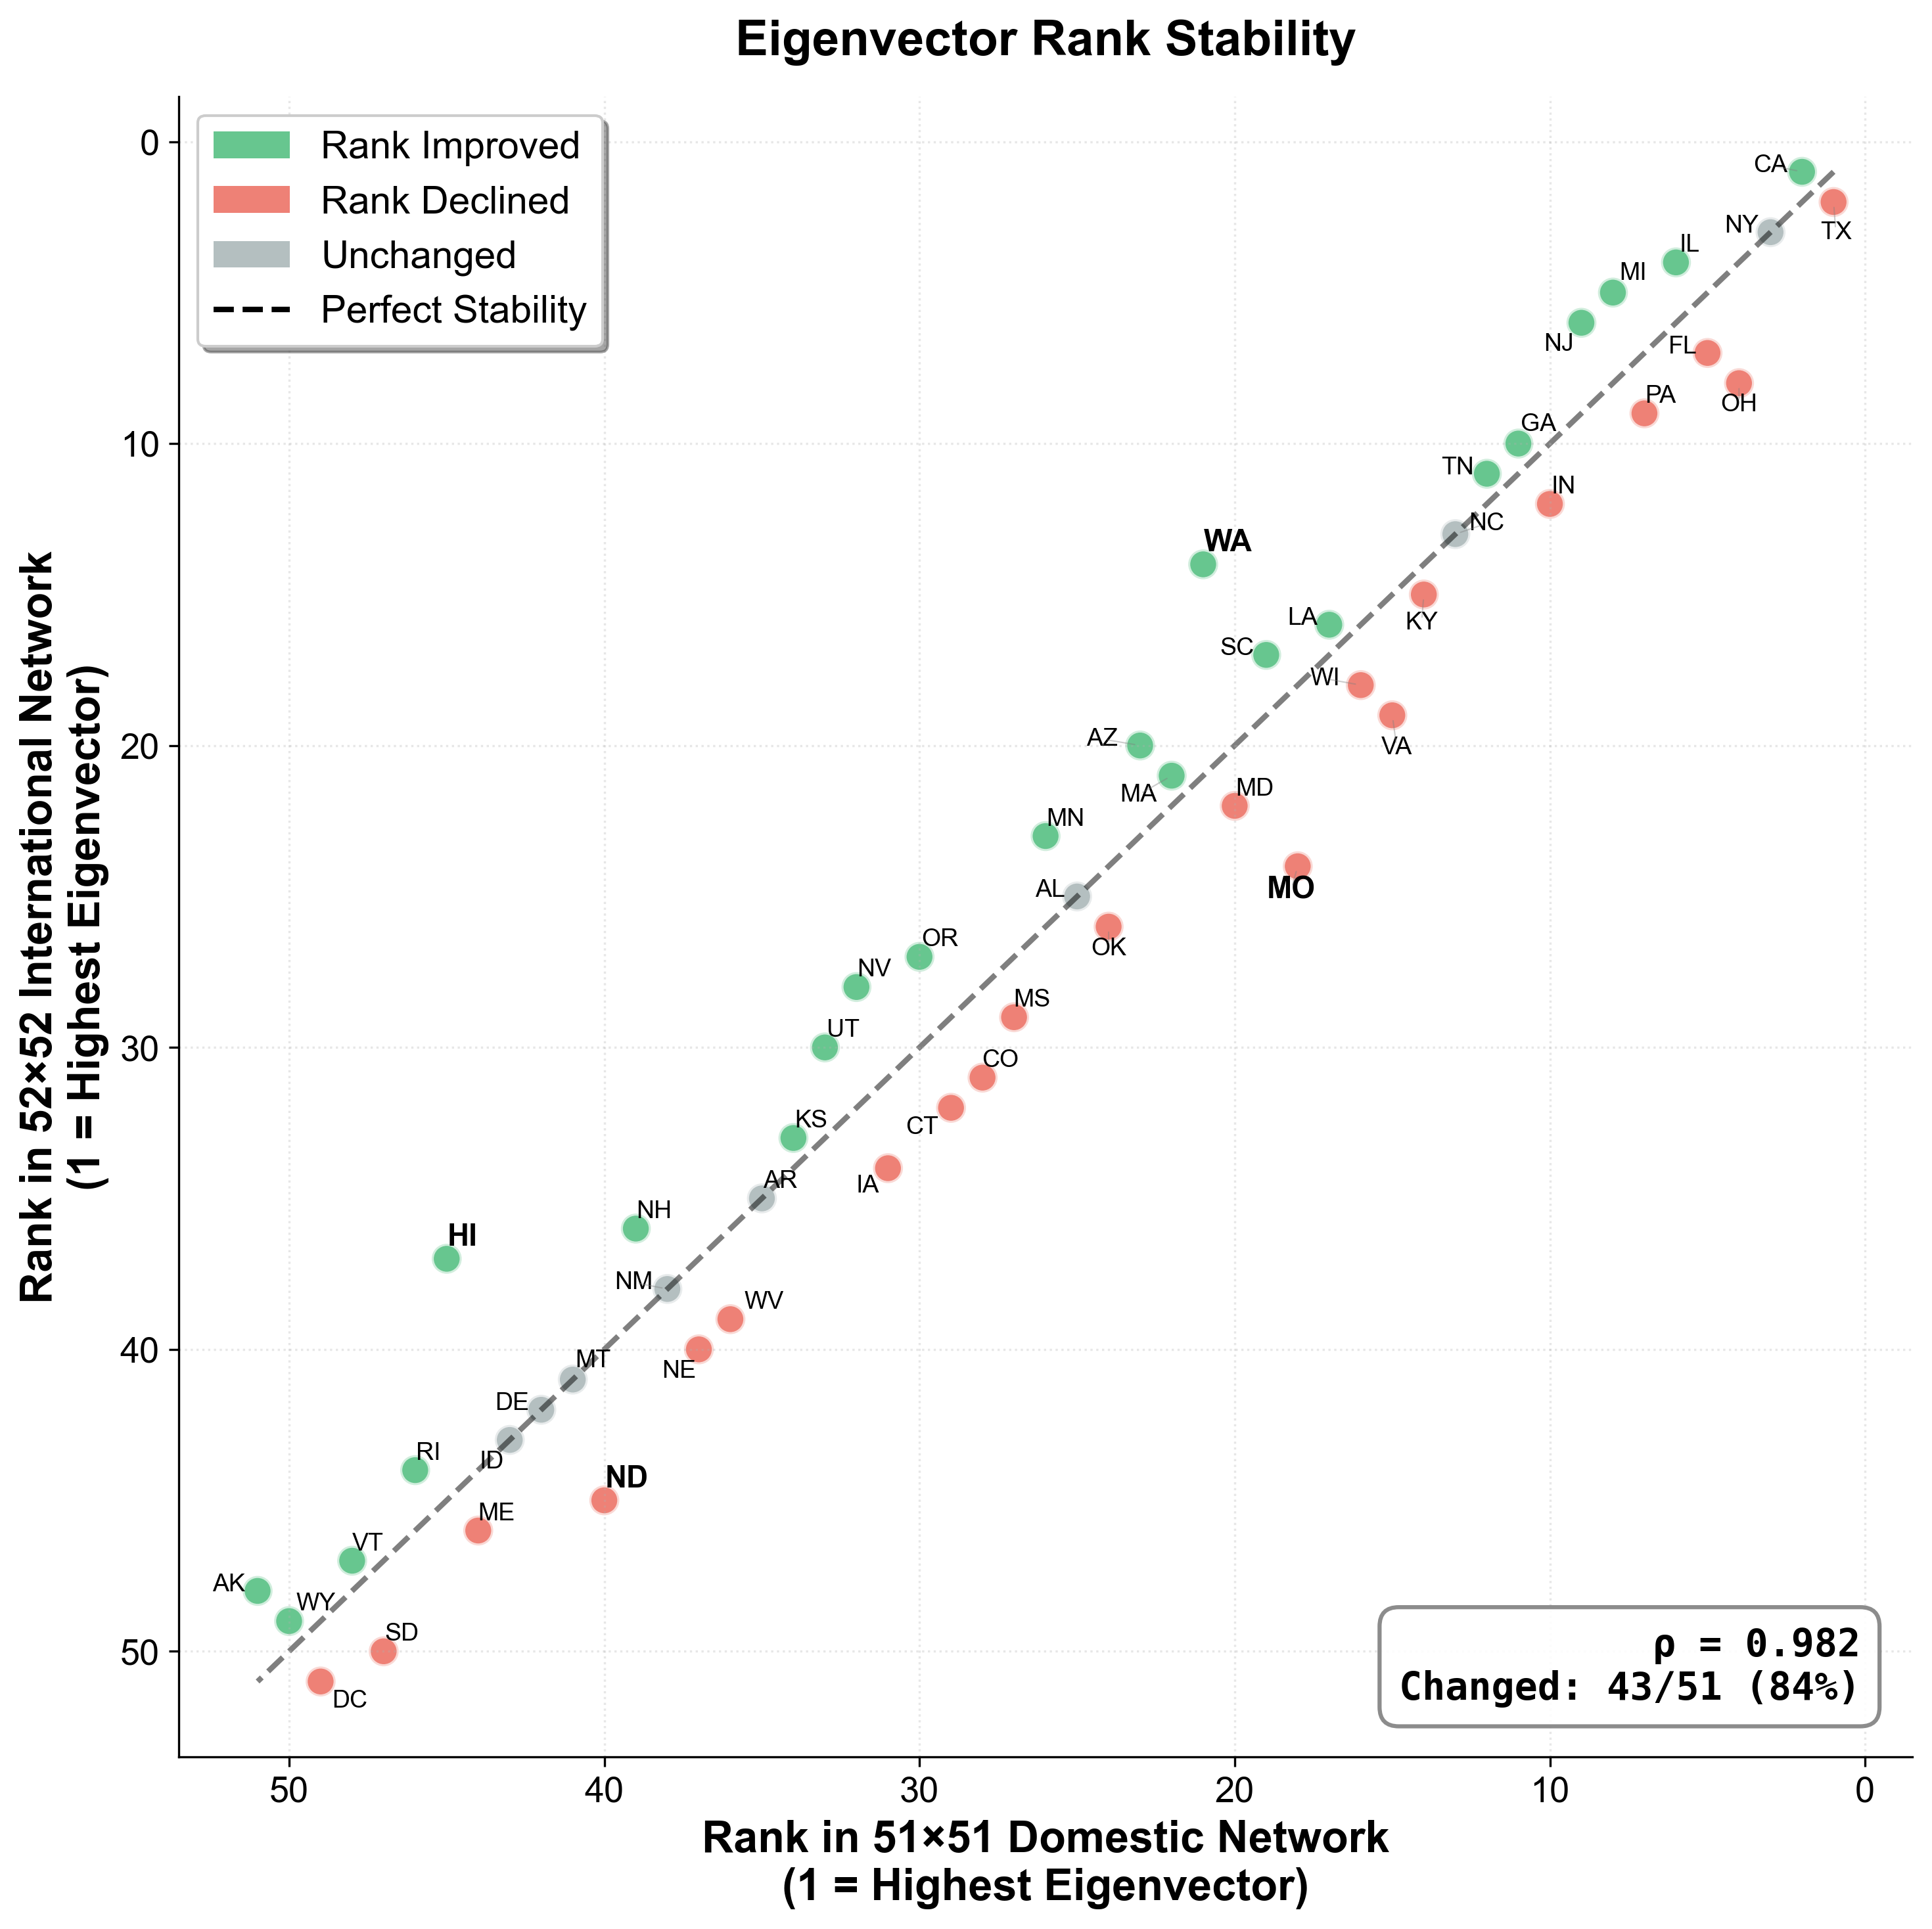
\includegraphics[width=\textwidth]{figures/rank_scatter_eigenvector.png}
\caption[Eigenvector centrality rank stability ($\rho = 0.982$, 84\% changed).]{Eigenvector centrality rank stability ($\rho = 0.982$, 84\% changed). Gateway states (CA, TX, NY) show
moderate rank shifts as RoW connections redistribute influence through the network.}
\label{fig:rank_eigenvector}
\end{figure}

\begin{figure}[htbp]
\centering
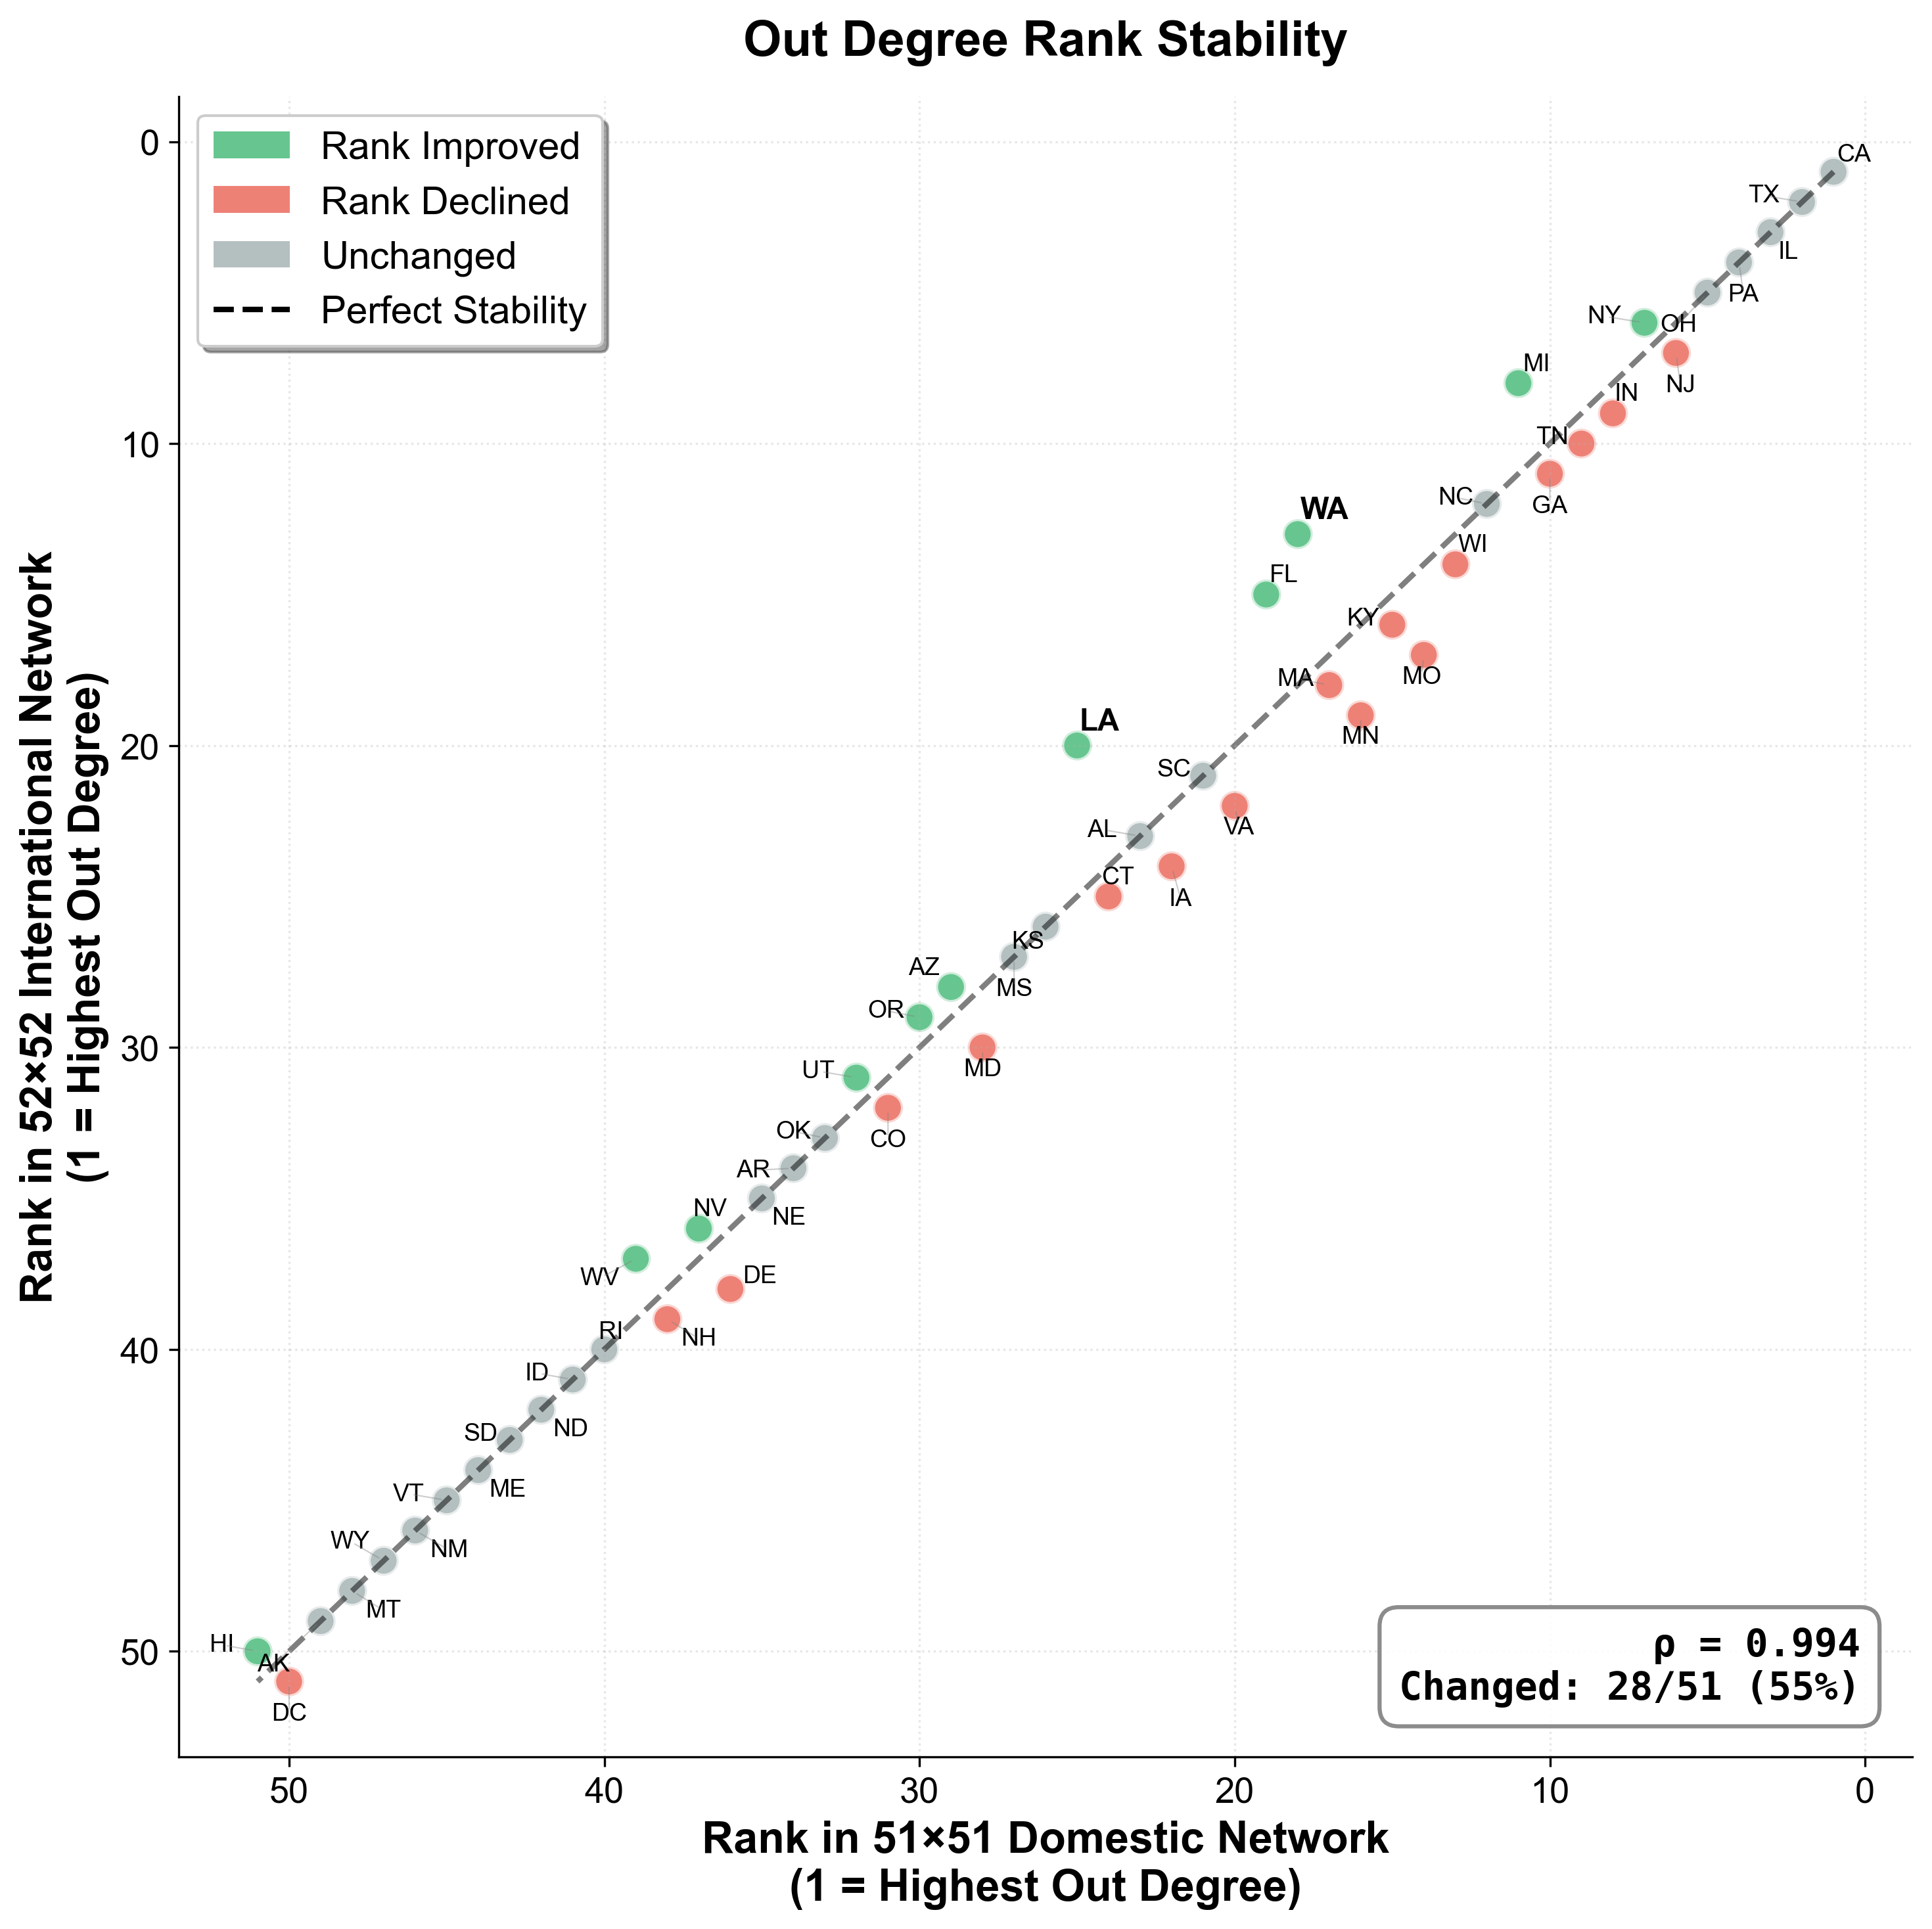
\includegraphics[width=\textwidth]{figures/rank_scatter_out_degree.png}
\caption[Weighted out-degree rank stability ($\rho = 0.994$, 88\% changed).]{Weighted out-degree rank stability ($\rho = 0.994$, 88\% changed). Highest stability among all
measures---top producers maintained positions, with only proportional rank adjustments.}
\label{fig:rank_outdegree}
\end{figure}



\chapter{Code and Data Availability}                                          
\label{appendix:code}                                                       
All code, data, and computational artifacts supporting this analysis are publicly available.                                                       
\subsection*{Thesis Pipeline}          

The complete analysis pipeline is available at:
\begin{center}
\url{https://github.com/rsthornton/us-trade-centrality}
\end{center}
The repository includes the \texttt{cfs-network-toolkit} Python package, 
configuration files, figure generation scripts, and the canonical result files from the November 2025 pipeline runs used throughout this analysis. Core results can be reproduced via \texttt{python main.py} from a fresh clone.

\subsection*{Interactive Visualization}

An interactive visualization of the interstate commodity trade network is publicly deployed at:

\begin{center}
\url{https://us-trade.plotly.app/}
\end{center}

Source code is available at \url{https://github.com/rsthornton/us-trade-centrality/tree/main/viz}. The tool supports commodity-level filtering across all SCTG codes, boundary sensitivity toggling between domestic and international network specifications, and a filtration stability slider.

\subsection*{Data Sources}

The primary dataset is the 2017 Commodity Flow Survey (CFS) Public Use File (PUF), produced by the U.S. Census Bureau:

\begin{center}
\url{https://www2.census.gov/programs-surveys/cfs/datasets/2017/}
\end{center}
International trade flows are drawn from the Freight Analysis Framework 
version 5.7.1 (FAF5), available from the Bureau of Transportation Statistics at \url{https://www.bts.gov/faf}.

\backmatter
\addcontentsline{toc}{chapter}{Bibliography}
\begin{singlespace}
\begin{sloppypar}
\setlength{\bibsep}{12pt}
\bibliographystyle{unsrtnat}
\bibliography{references}
\end{sloppypar}
\end{singlespace}

\end{document}
